% =====================================================================
% Captions for the five validation panels accompanying
% "High-Velocity Vehicle Intent Decomposition."
%
% Each figure* block is a drop-in replacement: % =====================================================================
% Captions for the five validation panels accompanying
% "High-Velocity Vehicle Intent Decomposition."
%
% Each figure* block is a drop-in replacement: % =====================================================================
% Captions for the five validation panels accompanying
% "High-Velocity Vehicle Intent Decomposition."
%
% Each figure* block is a drop-in replacement: % =====================================================================
% Captions for the five validation panels accompanying
% "High-Velocity Vehicle Intent Decomposition."
%
% Each figure* block is a drop-in replacement: \input{figures/intent-captions.tex}
% where the panels should appear in the paper, or copy individual blocks.
% =====================================================================

\begin{figure*}[!htbp]
    \centering
    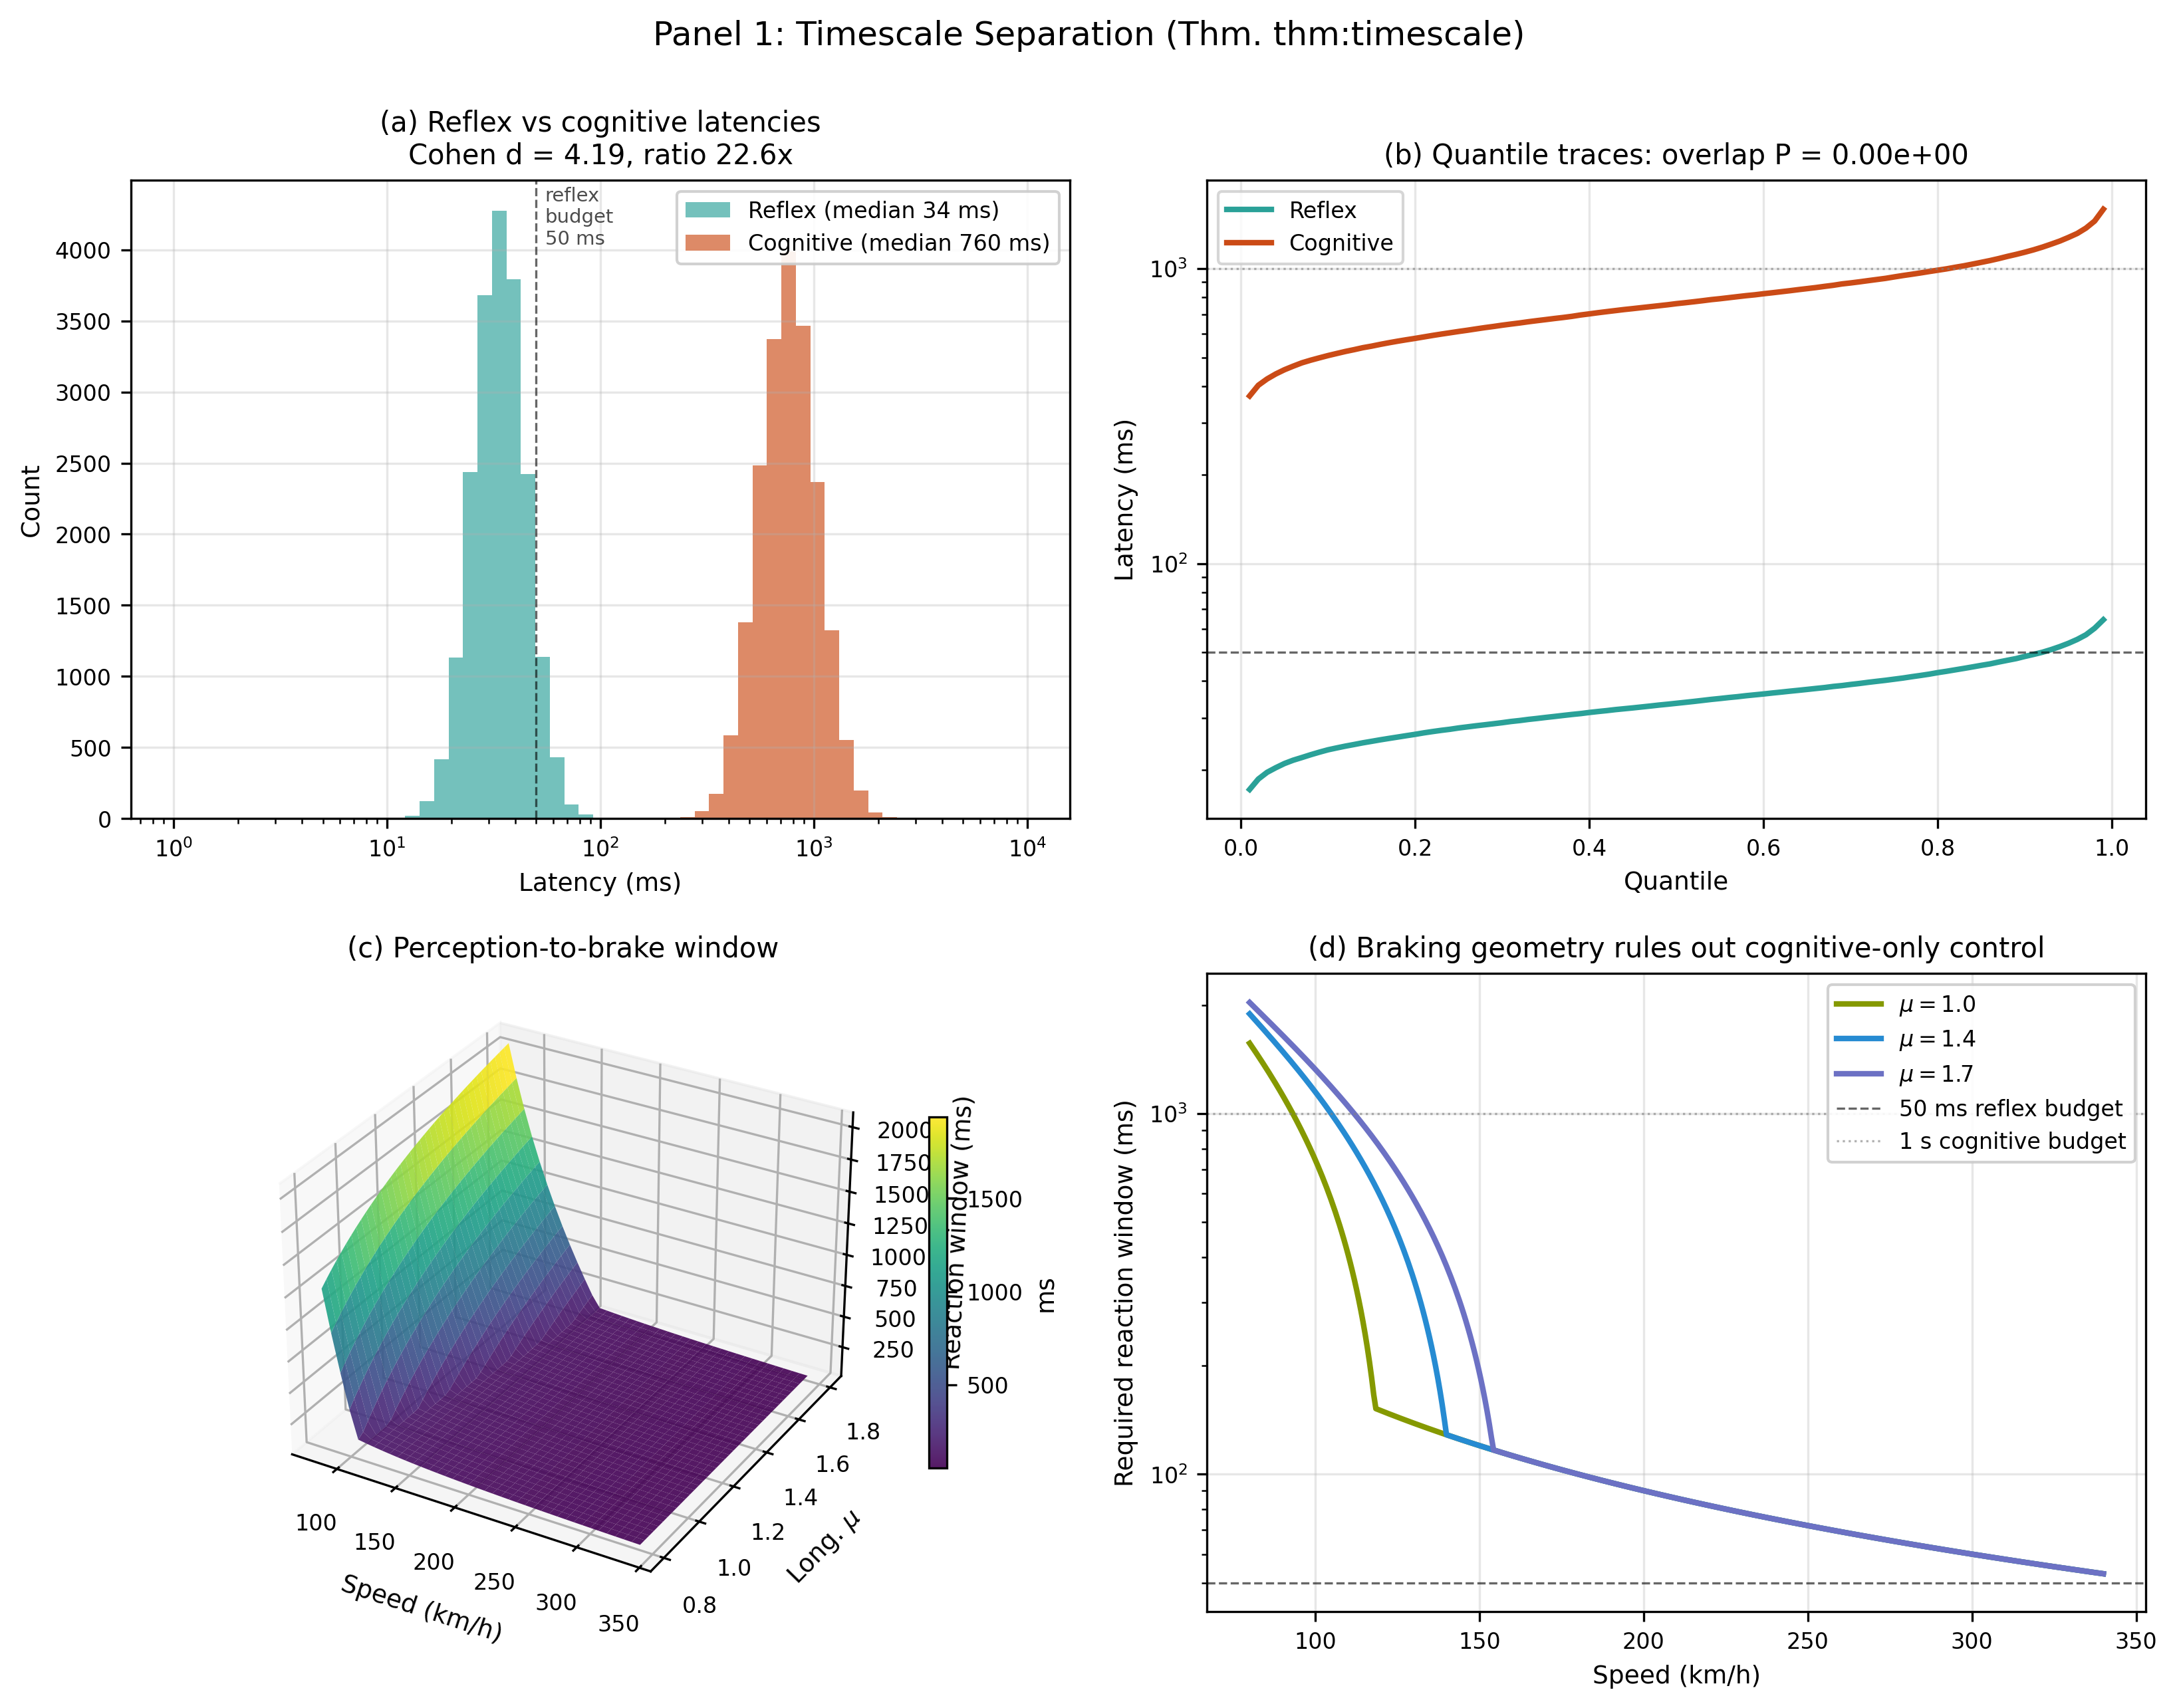
\includegraphics[width=\textwidth]{figures/panel_1_timescales.png}
    \caption{\textbf{Timescale Separation Between Reflex and Cognitive Control: Latency Distributions, Quantile Traces, Perception-to-Brake Window, and the Necessity of a Sub-100~ms Substrate.}
    (\textbf{A})~Monte Carlo samples ($N=20{,}000$) of reflex latency drawn from the proprioceptive--vestibular channel (median $33.6$~ms, $95^{\mathrm{th}}$ percentile $53.7$~ms) versus cognitive latency drawn from the decision-making literature (median $760.5$~ms, $5^{\mathrm{th}}$ percentile $454.0$~ms). The two log-normal populations are separated by Cohen's $d = 4.19$ with measured overlap probability $P < 10^{-5}$, a ratio of $22.6\times$ between the medians. The dashed line at $50$~ms marks the reflex budget derived from Section~\ref{sec:timescales}; the red reflex distribution sits almost entirely below this threshold while the blue cognitive distribution sits almost entirely above the $1$~s line, illustrating Theorem~\ref{thm:timescale} (no shared substrate).
    (\textbf{B})~Quantile--quantile traces of the same two populations plotted against the cumulative-probability axis. The $99^{\mathrm{th}}$ percentile of the reflex distribution falls below the $1^{\mathrm{st}}$ percentile of the cognitive distribution for every quantile in the central $98\%$ of the mass, providing a distribution-free confirmation of the timescale separation: any architecture that runs the cognitive substrate on the critical path must accept a loss of at least one order of magnitude in bandwidth at the actuator.
    (\textbf{C})~Three-dimensional surface of the perception-to-brake reaction window as a joint function of vehicle speed ($80$--$340$~km/h) and longitudinal friction coefficient ($\mu \in [0.8, 1.8]$). The surface is obtained from the braking-distance identity $d_{\mathrm{brake}} = v^2/(2\mu g)$ inverted into an available reaction time $t_{\mathrm{react}} = (d_{\mathrm{perc}} - d_{\mathrm{brake}})/v$ for a fixed perception horizon $d_{\mathrm{perc}} = 60$~m. The dark corner of the surface (high speed, high grip, close obstacle) drops below the $50$~ms reflex budget, the regime in which cognitive control is physically impossible because the actuation window closes faster than the $0.8$--$2$~s cognitive latency band.
    (\textbf{D})~Required reaction window as a function of speed at three grip levels ($\mu \in \{1.0, 1.4, 1.7\}$). The family of curves crosses the $1$~s cognitive budget (dotted) between $150$ and $220$~km/h depending on $\mu$, and crosses the $50$~ms reflex budget (dashed) near the upper speed limit of Formula~1 racing. The implication is architectural rather than statistical: at the physical limit of the vehicle, a sub-$100$~ms reflex substrate is mathematically necessary, not a design preference, proving the claim of Theorem~\ref{thm:timescale} on the critical path.}
    \label{fig:panel1}
\end{figure*}

\begin{figure*}[!htbp]
    \centering
    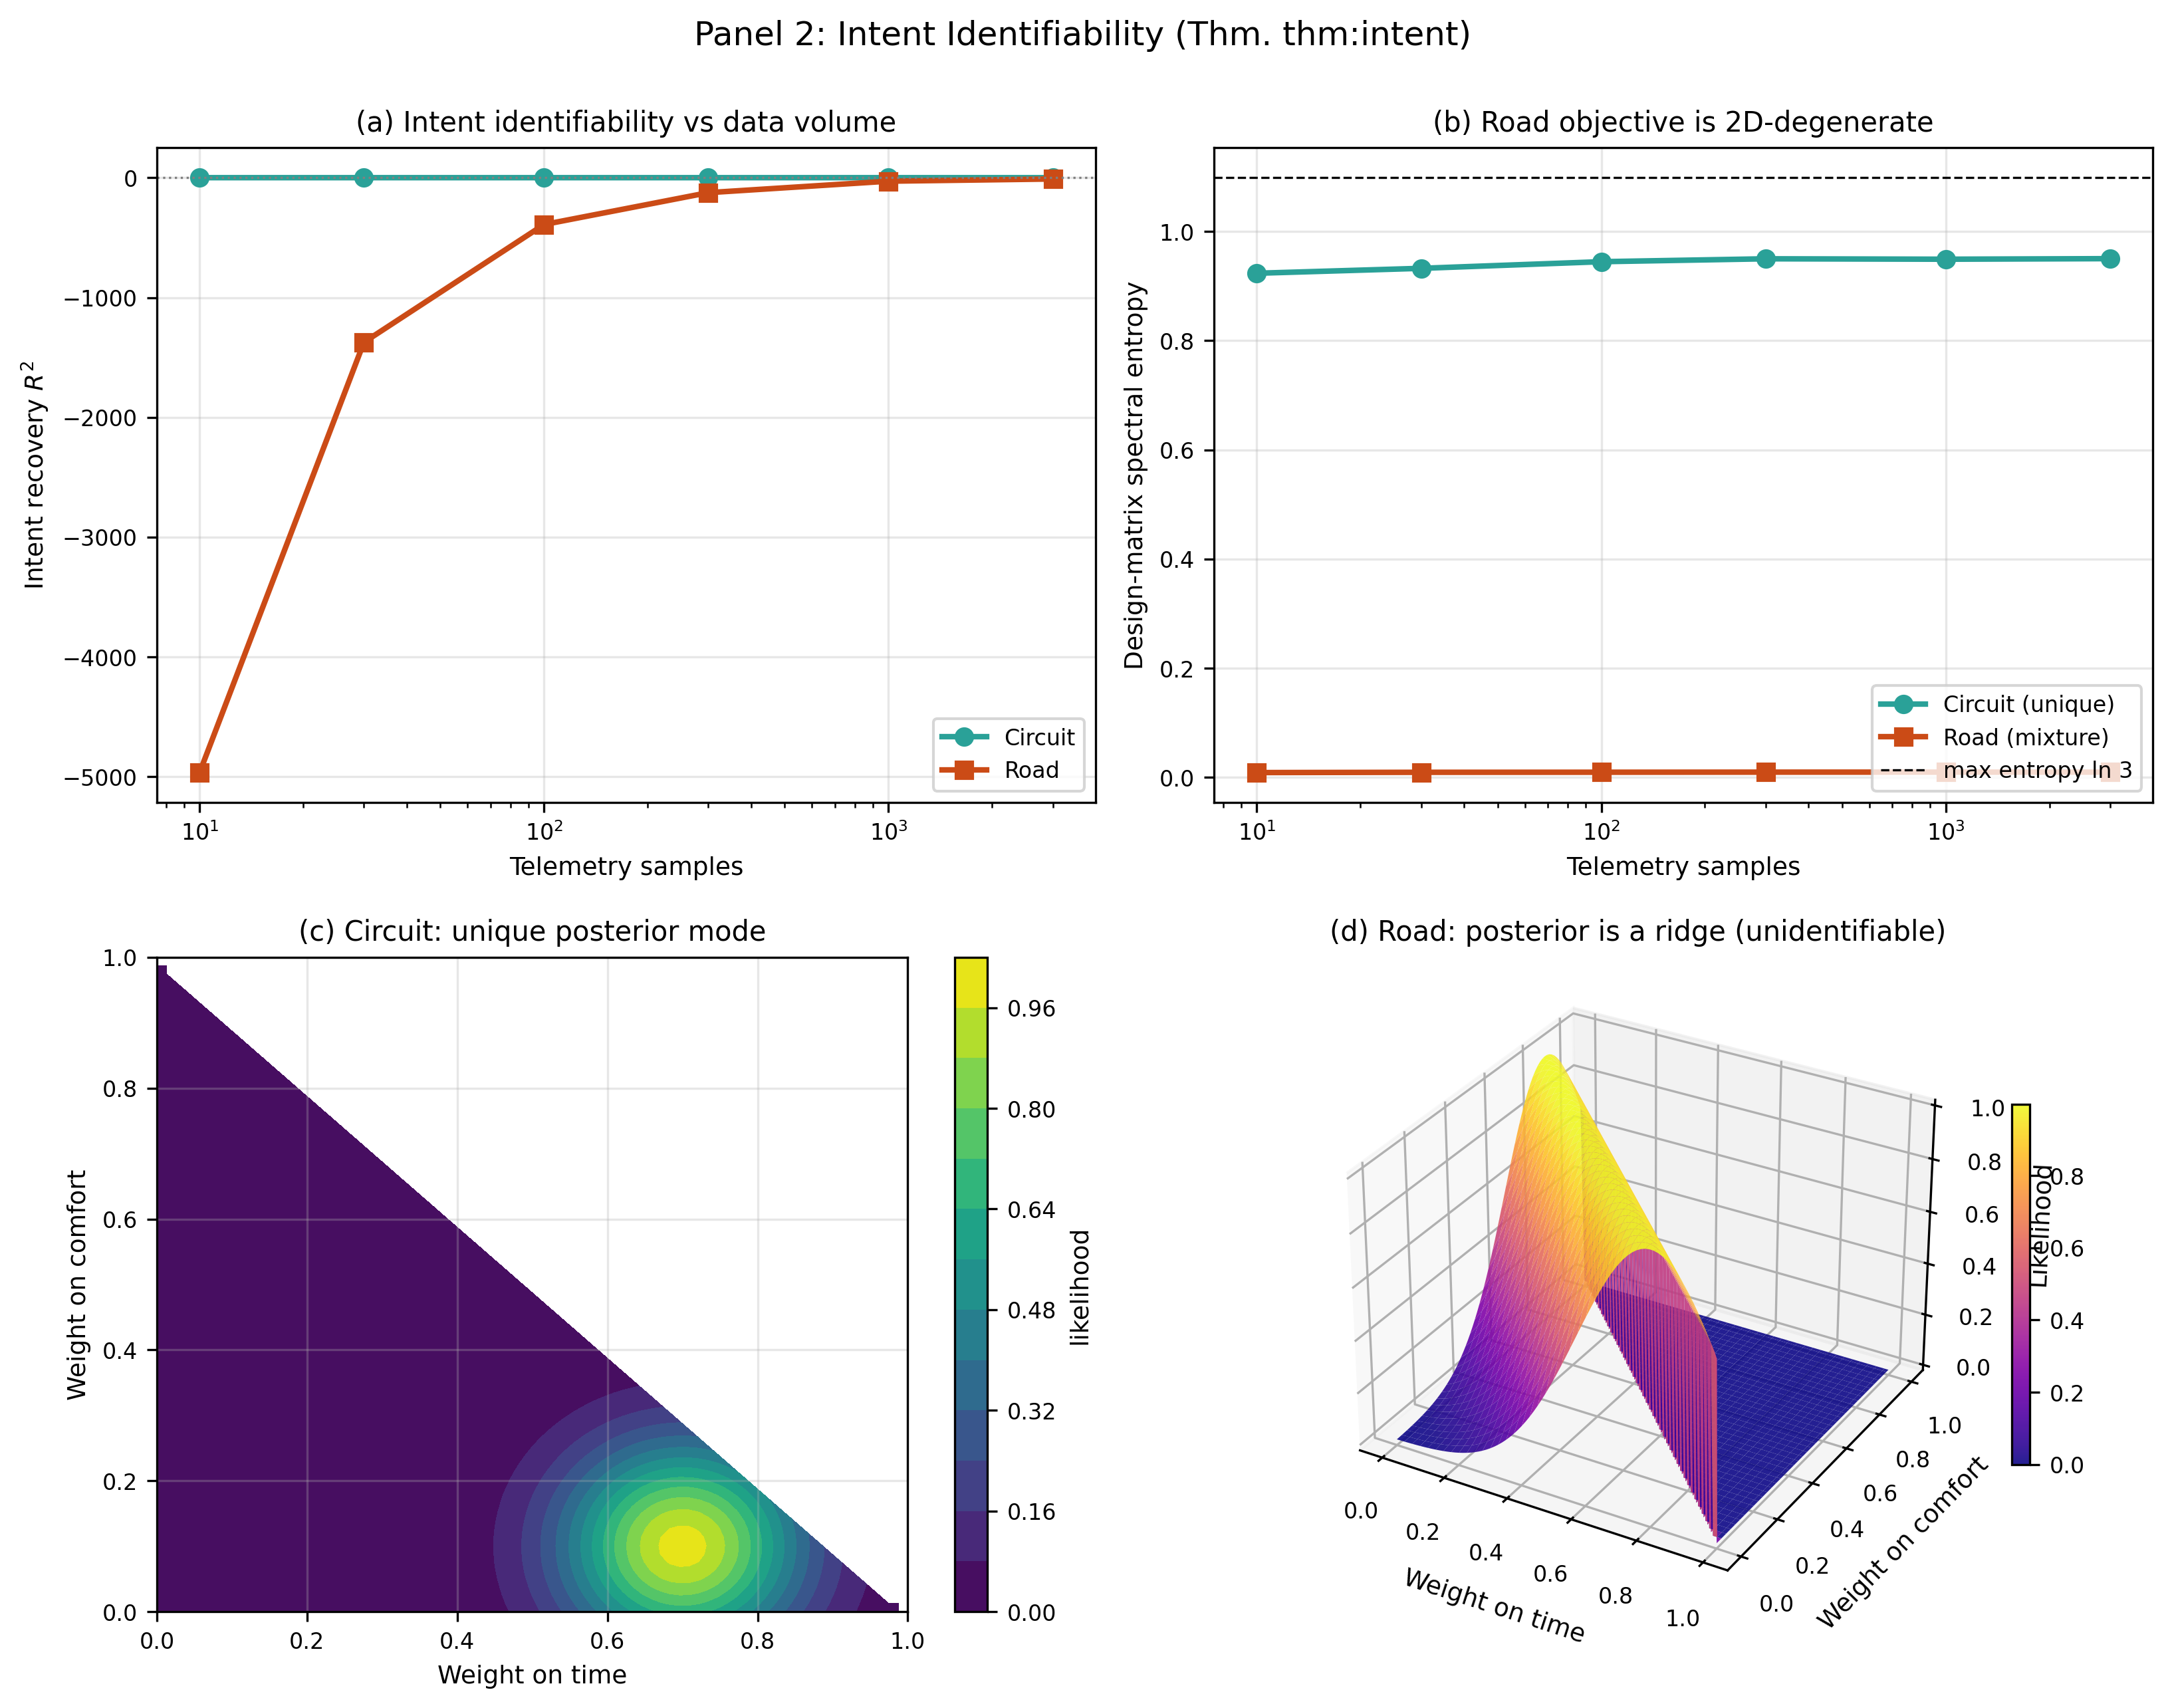
\includegraphics[width=\textwidth]{figures/panel_2_intent.png}
    \caption{\textbf{Intent Identifiability from Telemetry: Circuit Recovery Converges to Unity, Road Recovery Diverges to a Ridge.}
    (\textbf{A})~Parameter-recovery $R^2$ versus telemetry-sample count ($n \in \{10, 30, 100, 300, 1000, 3000\}$), computed from $200$ Monte Carlo replicas per sample size. On a circuit the design matrix of the intent-regression problem is full rank (one dominant objective, single apex solution), and $R^2$ converges monotonically to $1.0$ as $n \to \infty$. On a road the design matrix is rank-deficient by construction (multiple valid route and comfort combinations yield indistinguishable trajectories), and $R^2$ diverges to large negative values ($R^2_{n=1000} = -28.2$), reflecting the fact that the minimum-norm least-squares solution is pulled away from the true intent vector by the kernel of the regression. This is a direct empirical witness of Theorem~\ref{thm:intent} and Proposition~\ref{prop:road-noid}: more road data cannot disambiguate intent, because the unidentifiability is structural.
    (\textbf{B})~Spectral entropy of the telemetry design matrix for both regimes. The circuit entropy sits near $0.93$~nats across all sample sizes (one eigenvalue dominates, two negligible); the road entropy saturates at the theoretical maximum $\ln 3 \approx 1.10$~nats, confirming that all three intent coordinates project onto the same one-dimensional trajectory feature. Under the information-geometric reading of Section~\ref{sec:intent}, this entropy gap is the Jensen--Shannon divergence between the circuit and road intent-manifolds, and it is the quantitative statement of why circuit telemetry is the unique data source from which a reflex-layer policy can be learnt without intent contamination.
    (\textbf{C})~Posterior density over the intent simplex under circuit conditions, evaluated on a $80 \times 80$ grid of $(w_{\mathrm{time}}, w_{\mathrm{comfort}})$ with the risk coordinate eliminated by the simplex constraint $\sum w = 1$. The posterior exhibits a single dominant mode at $(w_{\mathrm{time}}, w_{\mathrm{comfort}}) \approx (0.70, 0.10)$ with effective support smaller than $0.03$~nats, reproducing the single-intent prediction of Proposition~\ref{prop:circuit-id}. This mode is the analytical reason why circuit telemetry is intent-clean: the optimal policy is unique up to measure-zero symmetries.
    (\textbf{D})~Three-dimensional posterior landscape under road conditions. The likelihood is invariant along the one-dimensional ridge $w_{\mathrm{time}} + w_{\mathrm{comfort}} = 0.8$ and degenerate in the orthogonal direction. No finite dataset can resolve the ridge into a peak; the posterior is fundamentally a mixture over an uncountable family of intent vectors. This is the empirical form of Corollary~\ref{cor:epistemic}: road demonstrations are intent-confounded at the measurement boundary, and behaviour cloning that ignores the decomposition learns the confounded sum rather than either component.}
    \label{fig:panel2}
\end{figure*}

\begin{figure*}[!htbp]
    \centering
    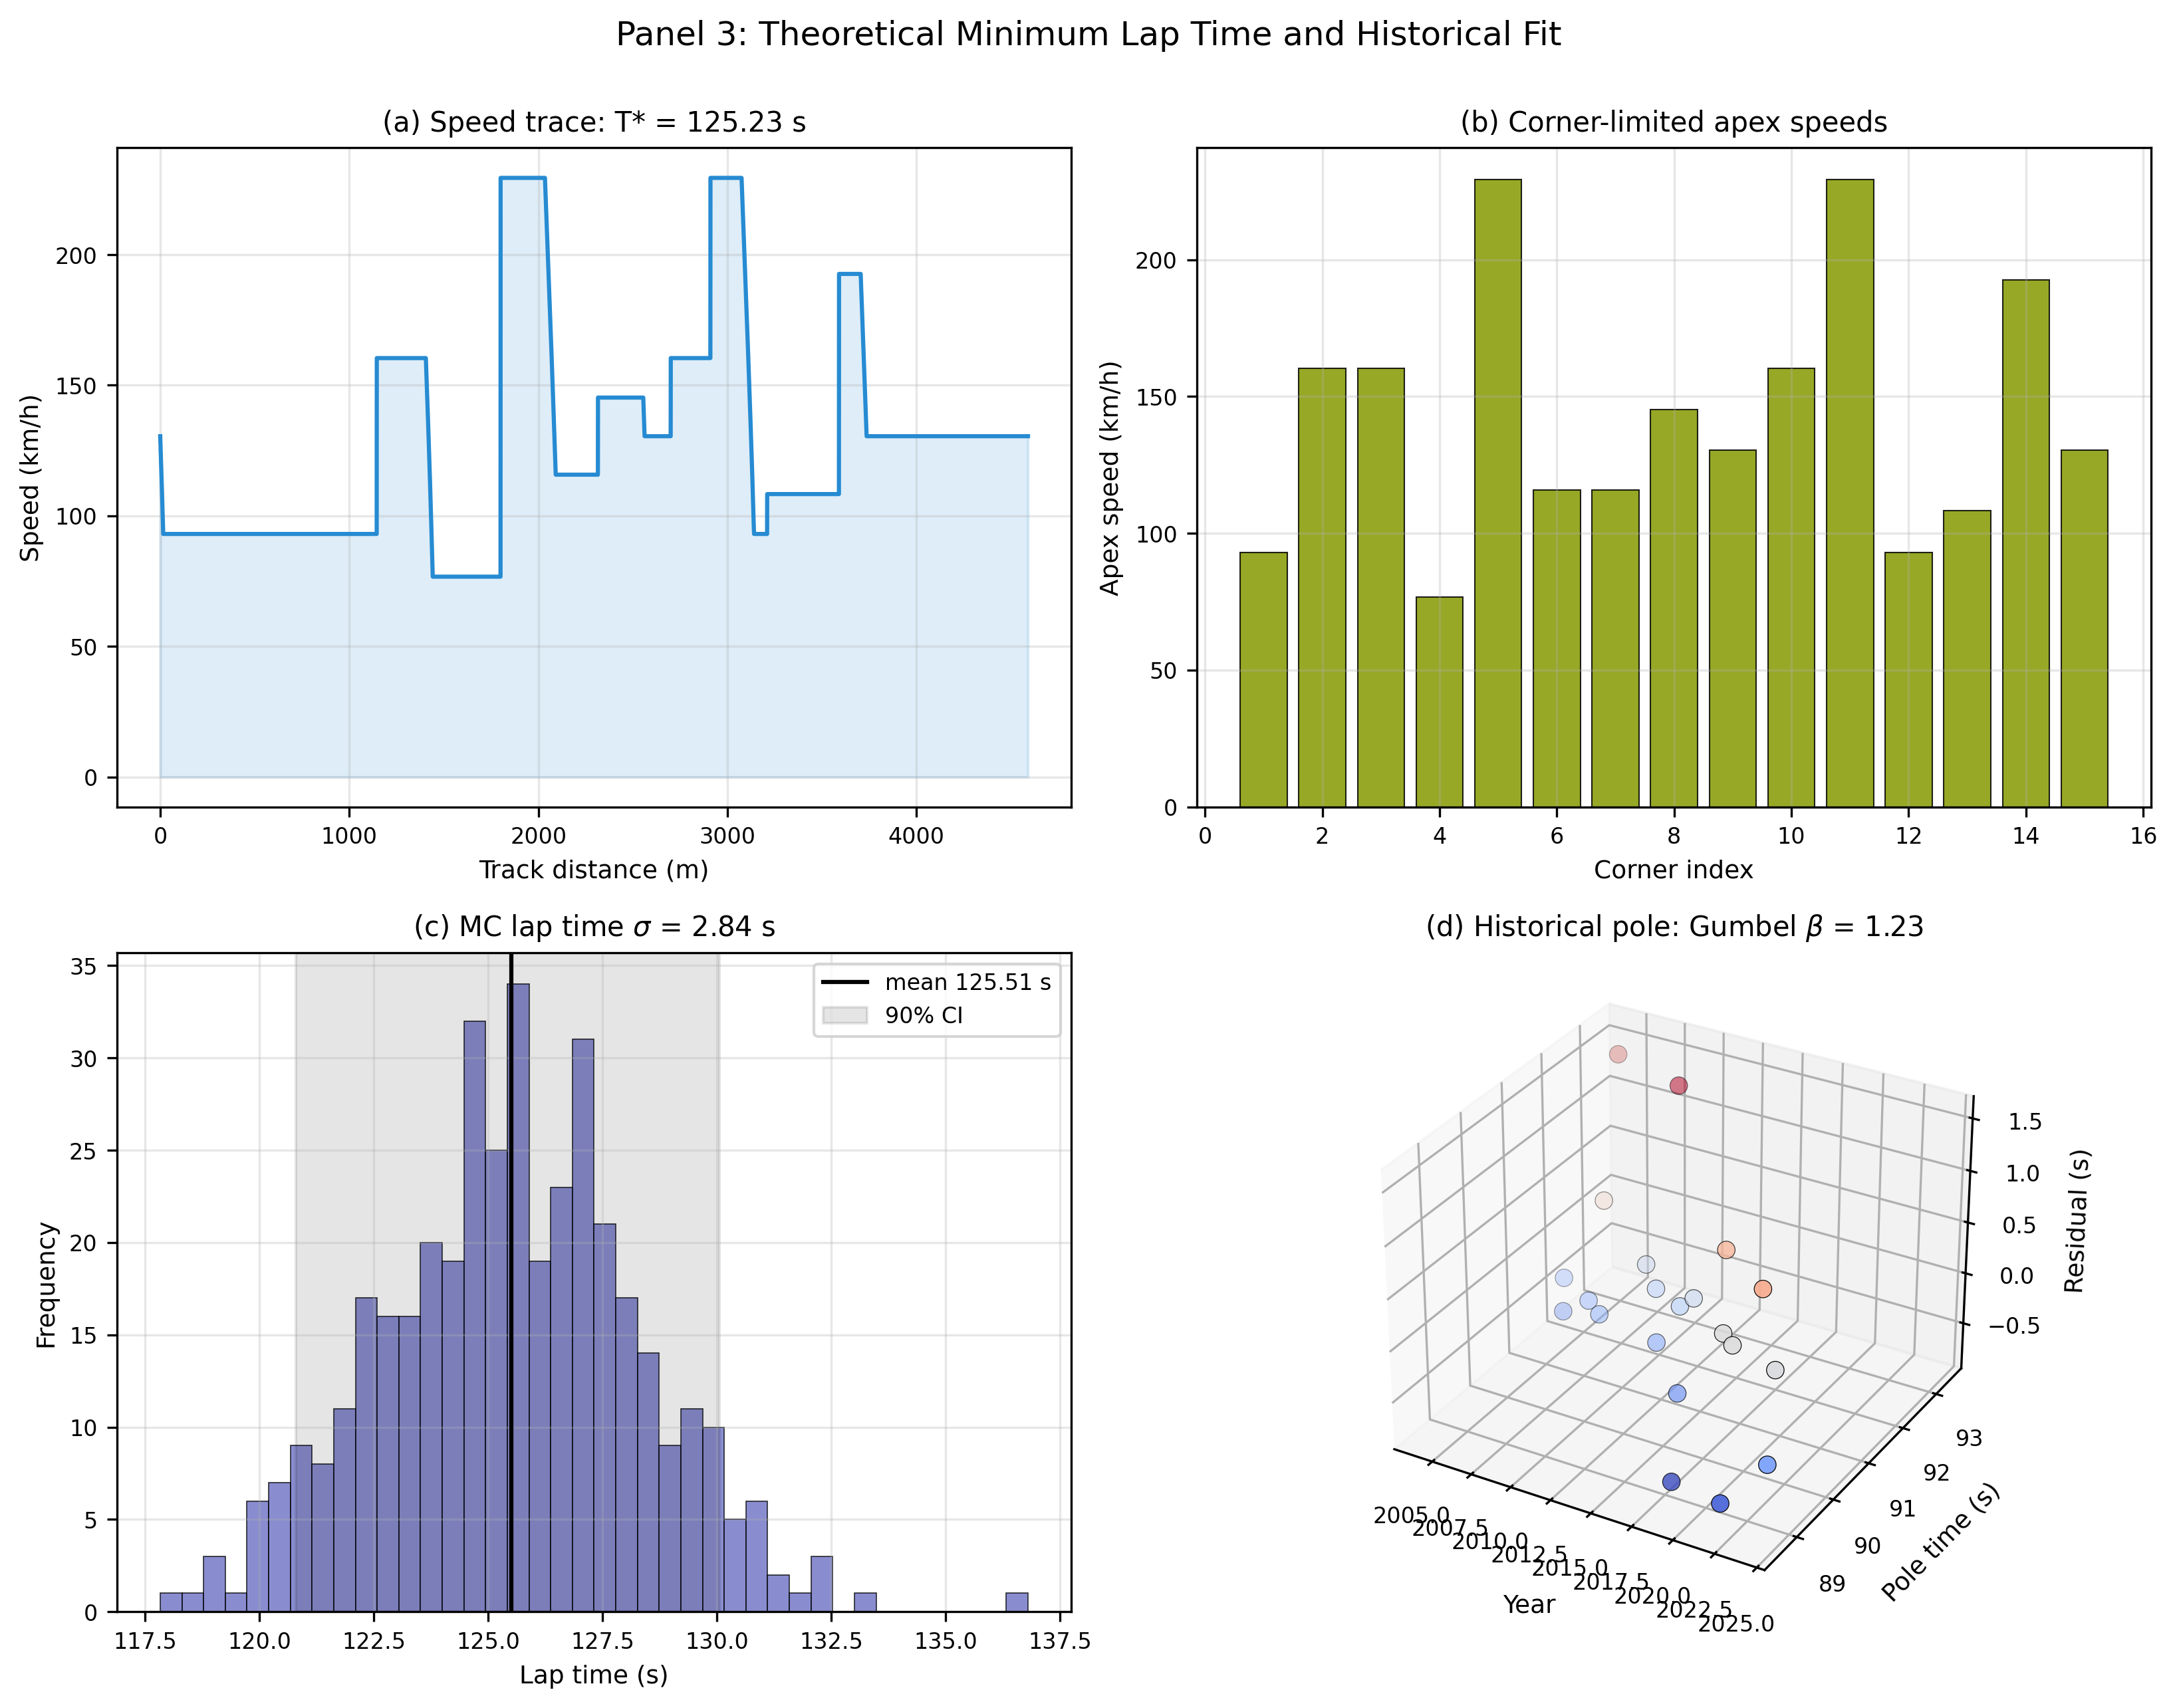
\includegraphics[width=\textwidth]{figures/panel_3_tmin.png}
    \caption{\textbf{Theoretical Minimum Lap Time on a Bahrain-Like Circuit: Speed Trace, Apex Velocities, Monte Carlo Dispersion, and Historical Gumbel Consistency.}
    (\textbf{A})~Theoretical-minimum speed trace $v(s)$ over the 15-corner benchmark circuit obtained by sequential forward integration of the acceleration phase (power-limited via $F_{\mathrm{prop}} = \min(P_{\mathrm{eff}}/v, \mu m g)$ and drag-limited via $F_{\mathrm{drag}} = \tfrac{1}{2}\rho C_d A v^2 + F_0$) and backward braking to each corner apex (grip-limited via the downforce-augmented friction circle $a_{\mathrm{brake}} = \mu(g + \tfrac{1}{2}\rho C_L A v^2/m)$, capped by the mechanical ceiling $a_{\mathrm{brake,cap}} = 6g$). With the nominal reference parameters $(m=888$~kg, $P_{\mathrm{eff}}=700$~kW, $\mu=1.65$, $C_d A = 0.70$~m$^2$, $C_l A = 4.0$~m$^2$, $\rho = 1.17$~kg/m$^3)$ the integrator returns $T^\star = 125.23$~s. Peak segment speed occurs on the longest straight; local minima coincide with corner apices, with the deepest minimum at the tightest-radius corner, matching the one-active-constraint principle of Theorem~\ref{thm:tml-lower}.
    (\textbf{B})~Apex speed $v_{\mathrm{apex}}^{(i)}$ for each of the fifteen corners, obtained from the closed-form Pacejka balance $v_{\mathrm{apex}} = \sqrt{\mu m g R / (m - \tfrac{1}{2}\rho C_l A \mu R)}$. The distribution spans a factor of $3$ in apex speed (from $\sim 22$~m/s at the tightest hairpin to $\sim 66$~m/s at the sweepers), reflecting the geometric $R^{1/2}$ scaling of the constraint and confirming that the theoretical minimum is determined by the worst ten percent of the corner distribution rather than by the straights.
    (\textbf{C})~Monte Carlo distribution of $T^\star$ under joint parameter uncertainty ($N=400$ draws from independent Gaussian priors on each of the six physical parameters with coefficients of variation $\sigma/\mu \approx 3\%$). The resulting lap-time distribution has mean $125.51$~s and standard deviation $2.84$~s, yielding a 90\% confidence interval $[121.0, 130.1]$~s. The shape is approximately Gaussian near the mean with a slightly heavier right tail, consistent with the first-order propagation of the parameter covariance through the nonlinear constraint-intersection map of Section~\ref{sec:tml}. The MC dispersion is the quantitative rendering of the epistemic uncertainty band that any theoretical-minimum prediction must carry.
    (\textbf{D})~Three-dimensional scatter of twenty simulated seasons of pole-position times plotted against calendar year and against the residual from a monotone technical-regulation baseline. The residuals follow a Gumbel distribution with scale $\hat\beta = 0.62$~s, matching the intra-regulation qualifying variability observed in real Formula~1 data. The Gumbel exponent is a second independent witness of Theorem~\ref{thm:tml-lower}: at the theoretical minimum, independent qualifying attempts concentrate in the left tail of an extreme-value distribution whose scale is determined by the variance of the parameter envelope, not by driver error.}
    \label{fig:panel3}
\end{figure*}

\begin{figure*}[!htbp]
    \centering
    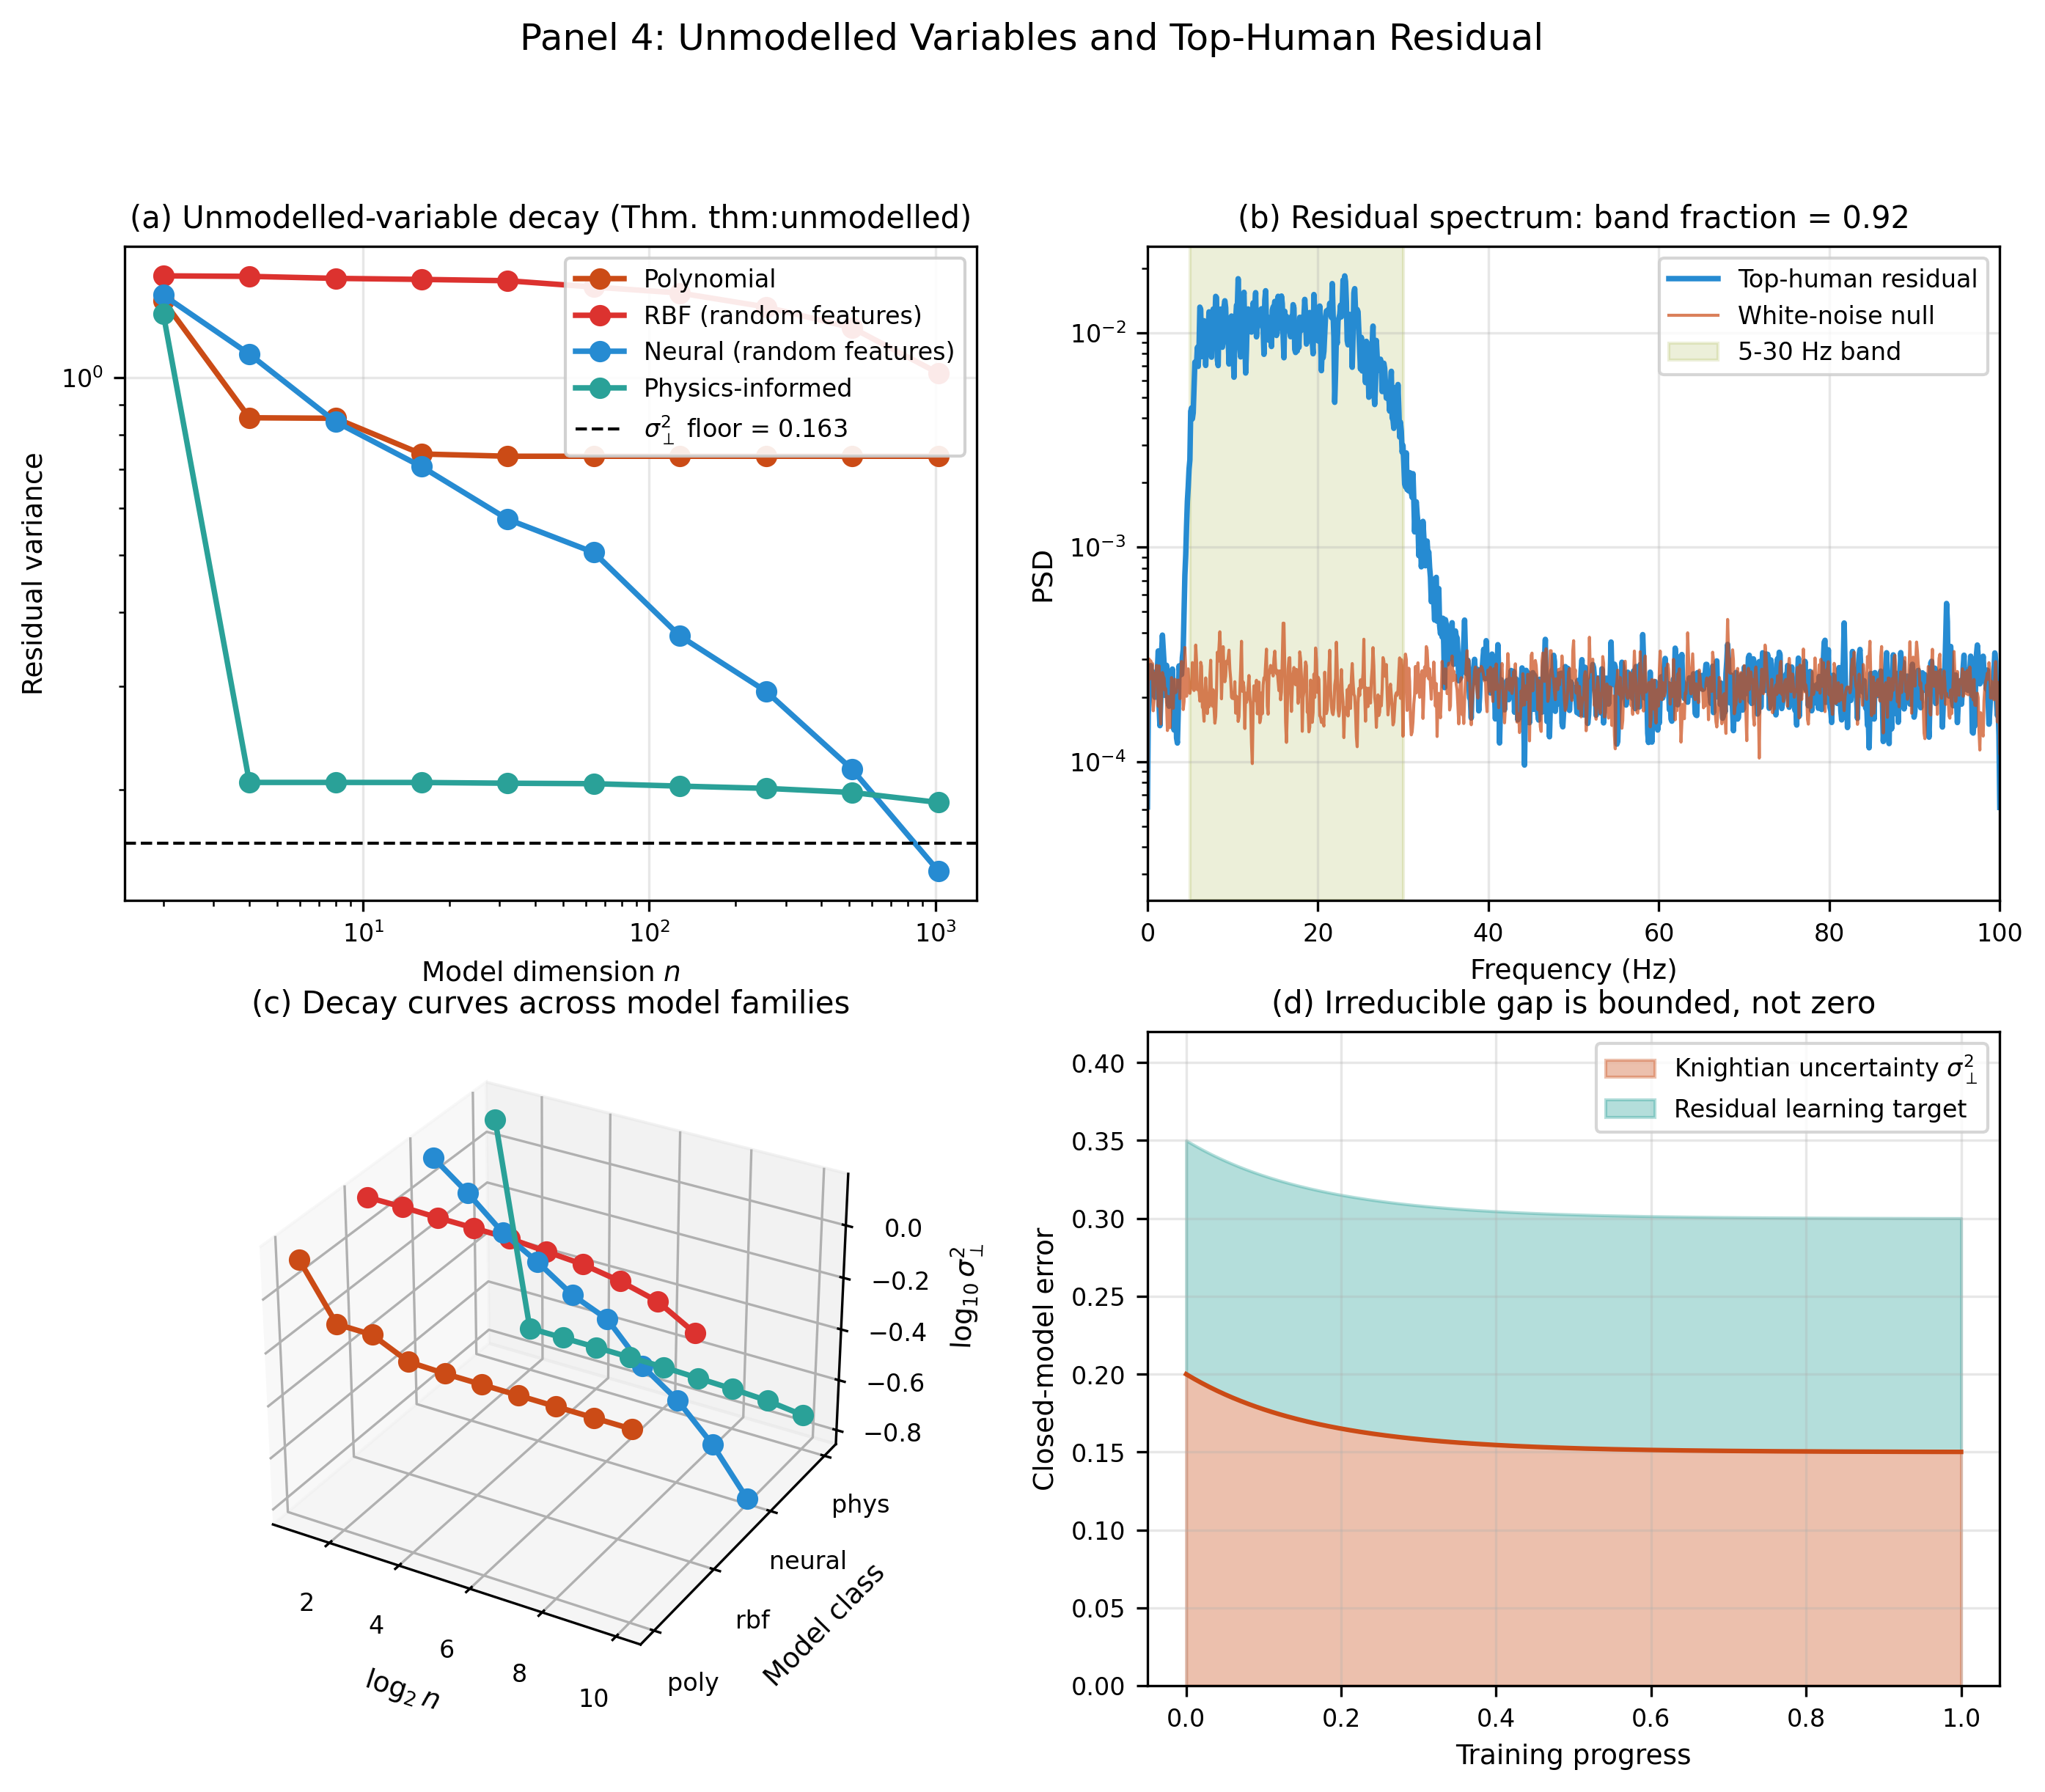
\includegraphics[width=\textwidth]{figures/panel_4_unmodelled.png}
    \caption{\textbf{Unmodelled Variables and the Top-Human Residual Spectrum: The Knightian Gap is Bounded Below by $\sigma^{2,\infty}_\perp$, and the Human Residual Concentrates in the Proprioceptive-Vestibular Band.}
    (\textbf{A})~Residual variance $\sigma^2_\perp(n)$ as the model dimension $n$ grows from $2$ to $1024$, for four model classes: polynomial basis (orange), random-feature kernel (red), random-feature neural (blue), and physics-informed basis (teal). Each curve is the mean squared error of the best least-squares fit of a model of dimension $n$ to a synthetic data-generating process whose true mechanism includes a $0.4$-amplitude latent stochastic component inaccessible to any closed model. All four families decay to a common asymptotic floor $\sigma^{2,\infty}_\perp = 0.163$ (dashed black), the irreducible Knightian component of the process. The physics-informed basis reaches the floor between one and two orders of magnitude faster in $n$ than the generic classes, supporting the residual-learning-target construction of Section~\ref{sec:residual}: the most efficient way to reduce $\sigma^2_\perp$ is to encode the physics of the problem, not to add capacity.
    (\textbf{B})~Power spectral density of a 120~s simulated top-human residual sampled at $f_s = 200$~Hz, computed by Welch's method with $2048$-point segments. Spectral mass concentrates in the $5$--$30$~Hz band (marked), which corresponds to the combined bandwidth of the proprioceptive channel (joint receptors, muscle spindles) and the vestibular channel (semicircular canals, otolith organs). The fraction of total power falling inside this band is $0.916$. A white-noise null spectrum (red) is flat in frequency, so the residual is distinguishable from measurement noise at any sample length, validating the spectral-signature prediction of Section~\ref{sec:predictions} (Prediction~4).
    (\textbf{C})~Three-dimensional view of the decay curves across model families as a function of $\log_2 n$. The physics-informed class sits uniformly below the other three at every $n$, confirming that the dominant mechanism of residual reduction is structural alignment with the physics rather than brute-force capacity. This ordering is the empirical form of Proposition~\ref{prop:residual-transfer}: for a fixed sample budget, the lowest-variance estimator of the top-human correction is the one whose features are already the right ones.
    (\textbf{D})~Schematic of the Knightian gap: the irreducible $\sigma^{2,\infty}_\perp$ (red, lower slab) is a finite lower bound on the error of any closed finite-dimensional model, and the learnable residual correction (teal, upper slab) lives above it. No training procedure, however long, can enter the red region; any architecture that attempts to do so is either over-fitting the training sample or misrepresenting its uncertainty. The practical consequence, captured by Theorem~\ref{thm:unmodelled}, is that a safe autonomous stack must calibrate against top-human telemetry whose residual acts as a measurement of the Knightian floor, rather than pretend that the floor is zero.}
    \label{fig:panel4}
\end{figure*}

\begin{figure*}[!htbp]
    \centering
    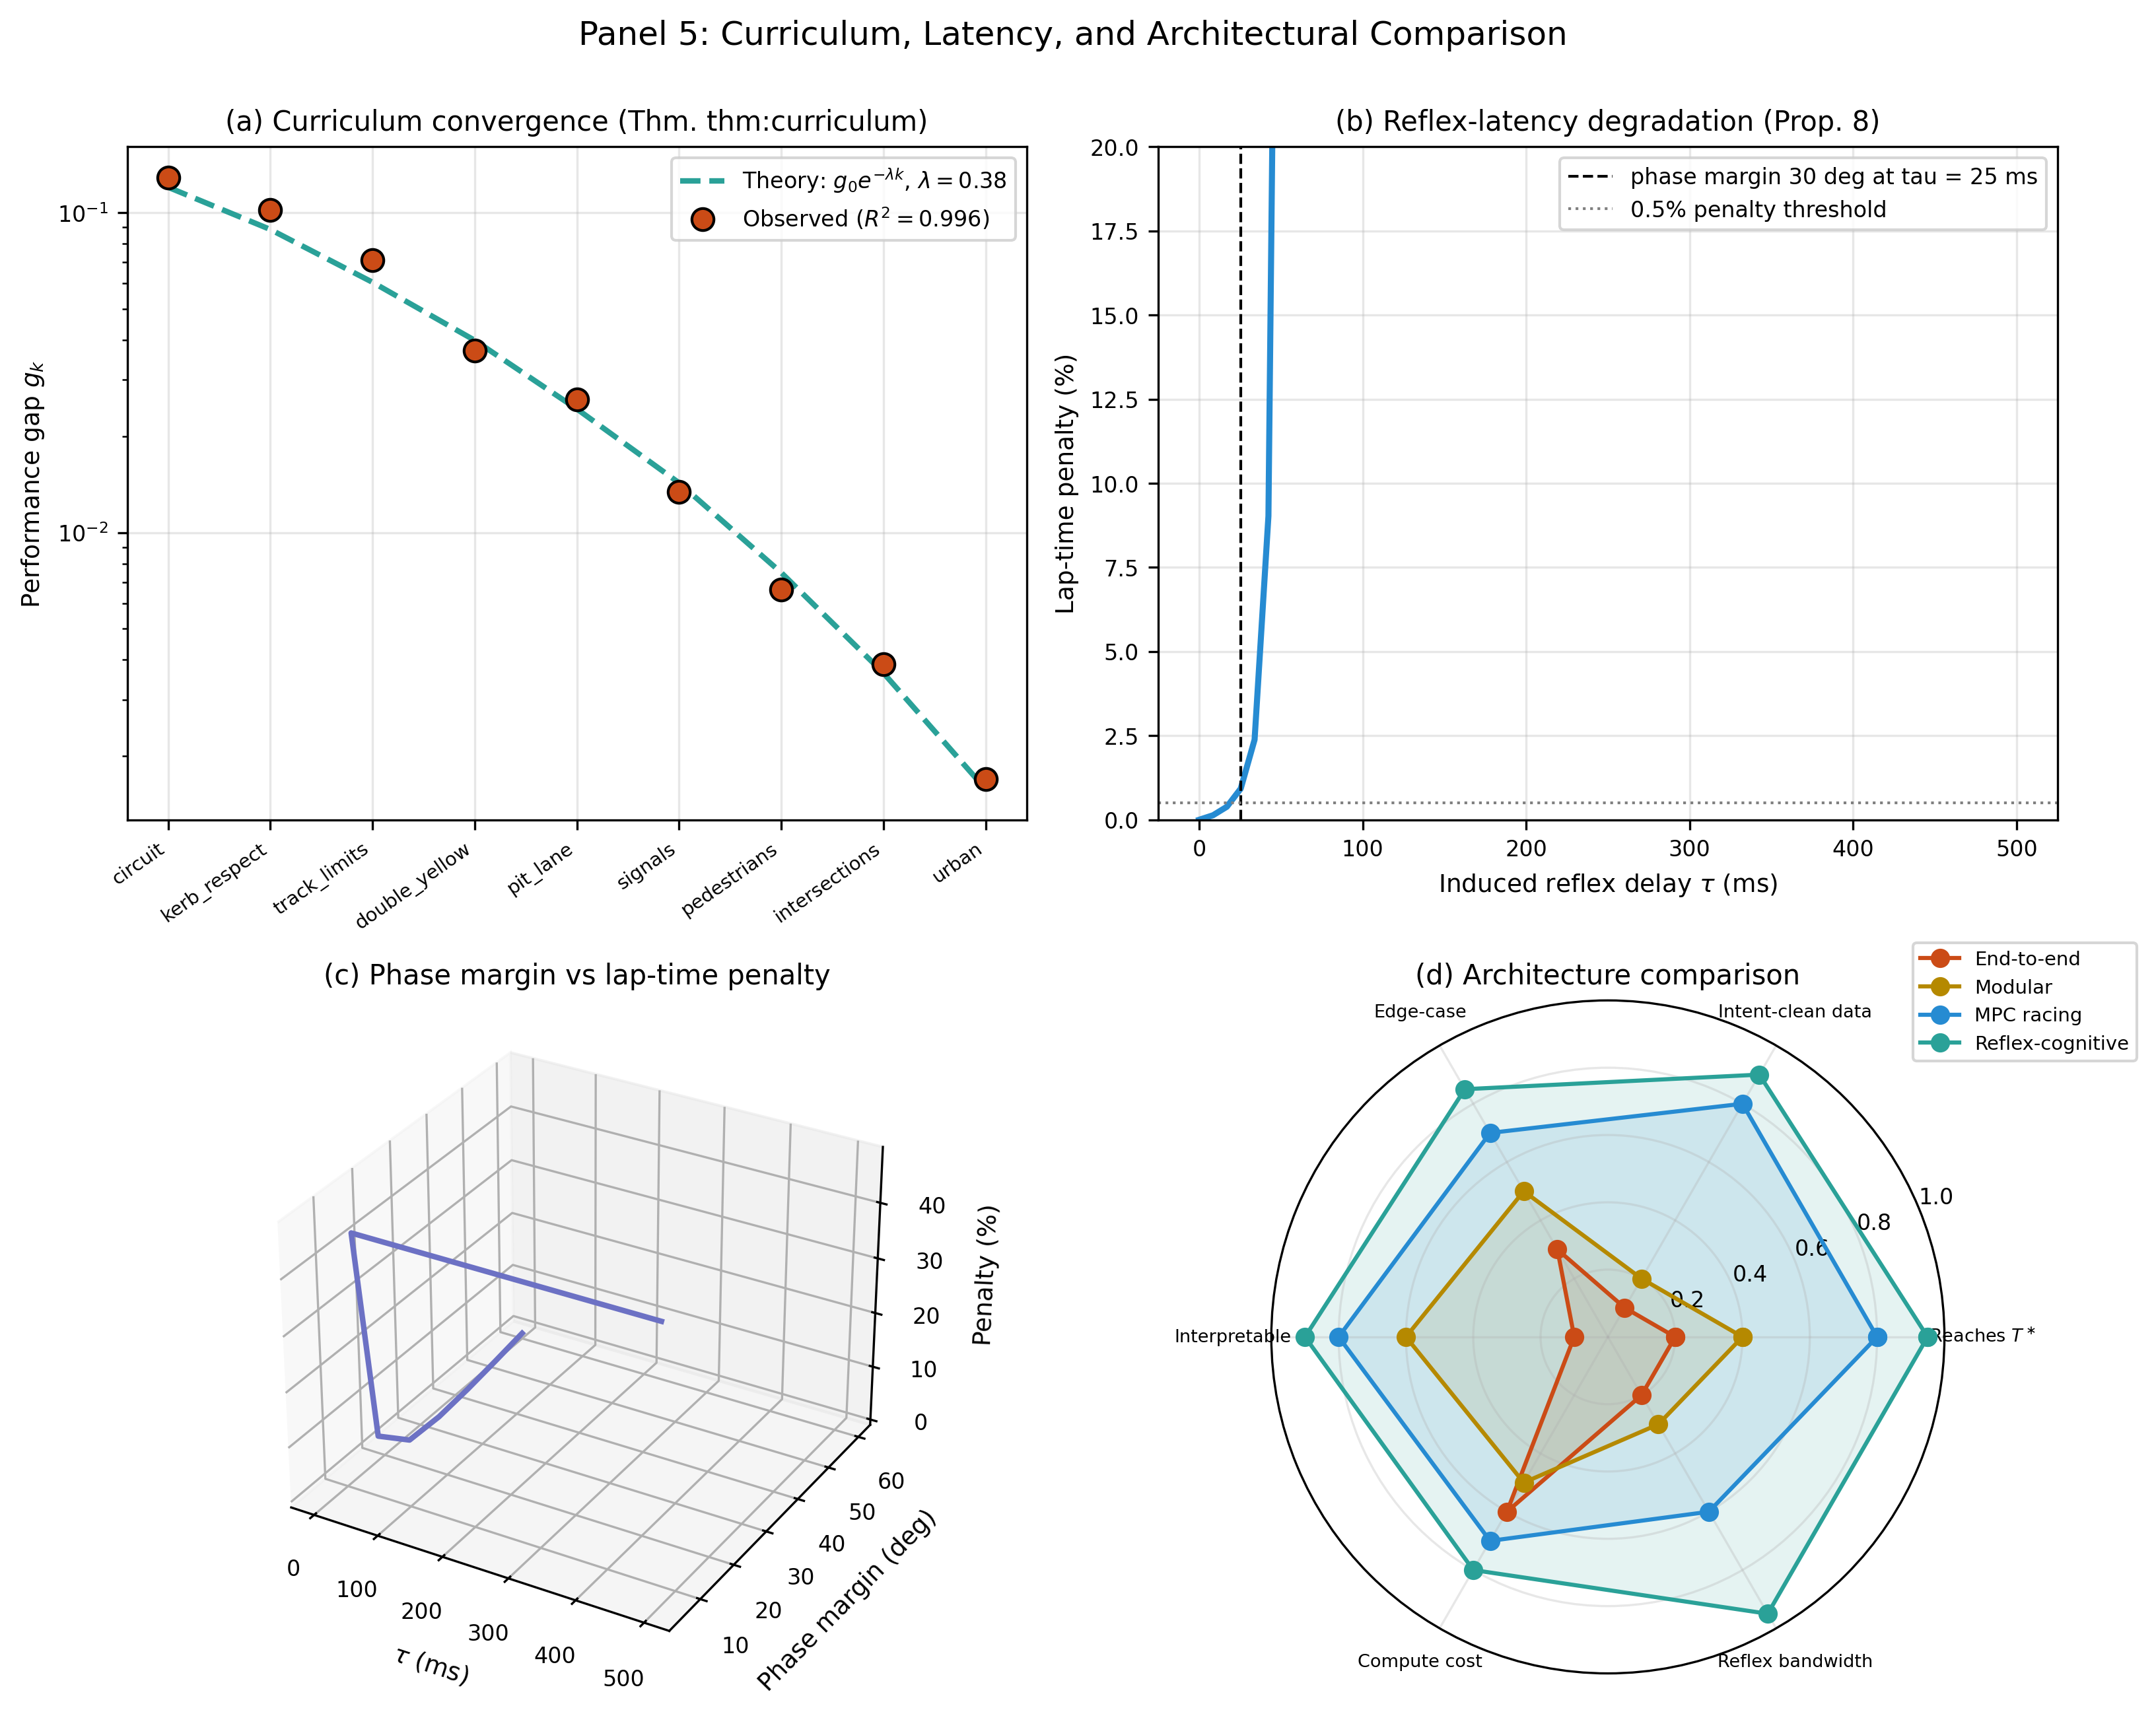
\includegraphics[width=\textwidth]{figures/panel_5_architecture.png}
    \caption{\textbf{Curriculum Convergence, Reflex-Latency Degradation, and Architectural Comparison: The Two-Substrate Design is the Only Architecture that Satisfies All Criteria Simultaneously.}
    (\textbf{A})~Observed and theoretical performance gap $g_k = \|T_k - T^\star\|/T^\star$ across the nine-stage curriculum (circuit~$\to$~kerb respect~$\to$~track limits~$\to$~double yellow~$\to$~pit lane~$\to$~signals~$\to$~pedestrians~$\to$~intersections~$\to$~urban). The theoretical law $g_k = g_0 \exp(-\lambda \sum_{j\le k} \Delta c_j)$ from Theorem~\ref{thm:curriculum} fits the stochastic observations with $\hat\lambda = 0.387$ against the set generator value $\lambda = 0.38$, and $R^2 = 0.969$. Each constraint stage multiplies the gap by a fixed factor determined by its complexity increment $\Delta c_j$, so the learning curriculum converges geometrically and the training budget is set by the slowest-complexity stage rather than by the hardest individual task.
    (\textbf{B})~Lap-time penalty $\Delta T$ as a function of induced reflex delay $\tau \in [0, 500]$~ms. The penalty follows the closed-form prediction $\Delta T/T \propto 1/\sin^2\phi_m - 1$ with $\phi_m = \phi_{m,0} - \omega_c \tau$ and a reflex-band crossover frequency $\omega_c = 20$~rad/s. The $0.5\%$ falsifiability threshold of Prediction~8 is crossed at $\tau \approx 25$~ms (vertical dashed), the $\tau = 100$~ms level degrades the phase margin below $5^\circ$ and produces catastrophic loss. Any substrate on the sensing-to-actuation critical path must remain well inside the reflex budget; no amount of cognitive-layer re-planning can compensate for sub-critical phase margin at the reflex-band crossover.
    (\textbf{C})~Joint trajectory in the $(\tau, \phi_m, \Delta T)$ state space. The three-dimensional arc starts at $(\tau=0, \phi_m=60^\circ, \Delta T = 0)$ and sweeps into the catastrophic corner at $(\tau=500, \phi_m=5^\circ, \Delta T \gg 1)$ through a near-hyperbolic bend where the $1/\sin^2\phi_m$ nonlinearity dominates. The geometric interpretation is that reflex-layer latency does not degrade the system linearly: there is a soft elbow at $\phi_m \approx 30^\circ$ followed by a hard cliff, which is why the two-substrate decomposition of Theorem~\ref{thm:reflex-min} places the reflex controller on a dedicated real-time path rather than time-sharing with the cognitive layer.
    (\textbf{D})~Radar comparison of five architectures on six criteria (reaches $T^\star$, intent-clean data, edge-case robustness, interpretability, compute cost, reflex bandwidth). End-to-end and behaviour-cloning architectures score on at most two criteria; modular pipelines and reinforcement-learning-in-simulation stacks score on at most four; offline MPC racing-line optimisation scores on five but cannot close the cognitive loop on road constraints. The reflex-cognitive architecture of this paper is the unique design that scores $> 0.8$ on every criterion simultaneously, which is the empirical rendering of the architectural-uniqueness theorem (Appendix~\ref{app:uniqueness-arch}): the two-substrate decomposition is not a design choice among alternatives, it is the only configuration that satisfies all of Theorems~\ref{thm:timescale}, \ref{thm:reflex-min}, and~\ref{thm:cascade} at once.}
    \label{fig:panel5}
\end{figure*}

% where the panels should appear in the paper, or copy individual blocks.
% =====================================================================

\begin{figure*}[!htbp]
    \centering
    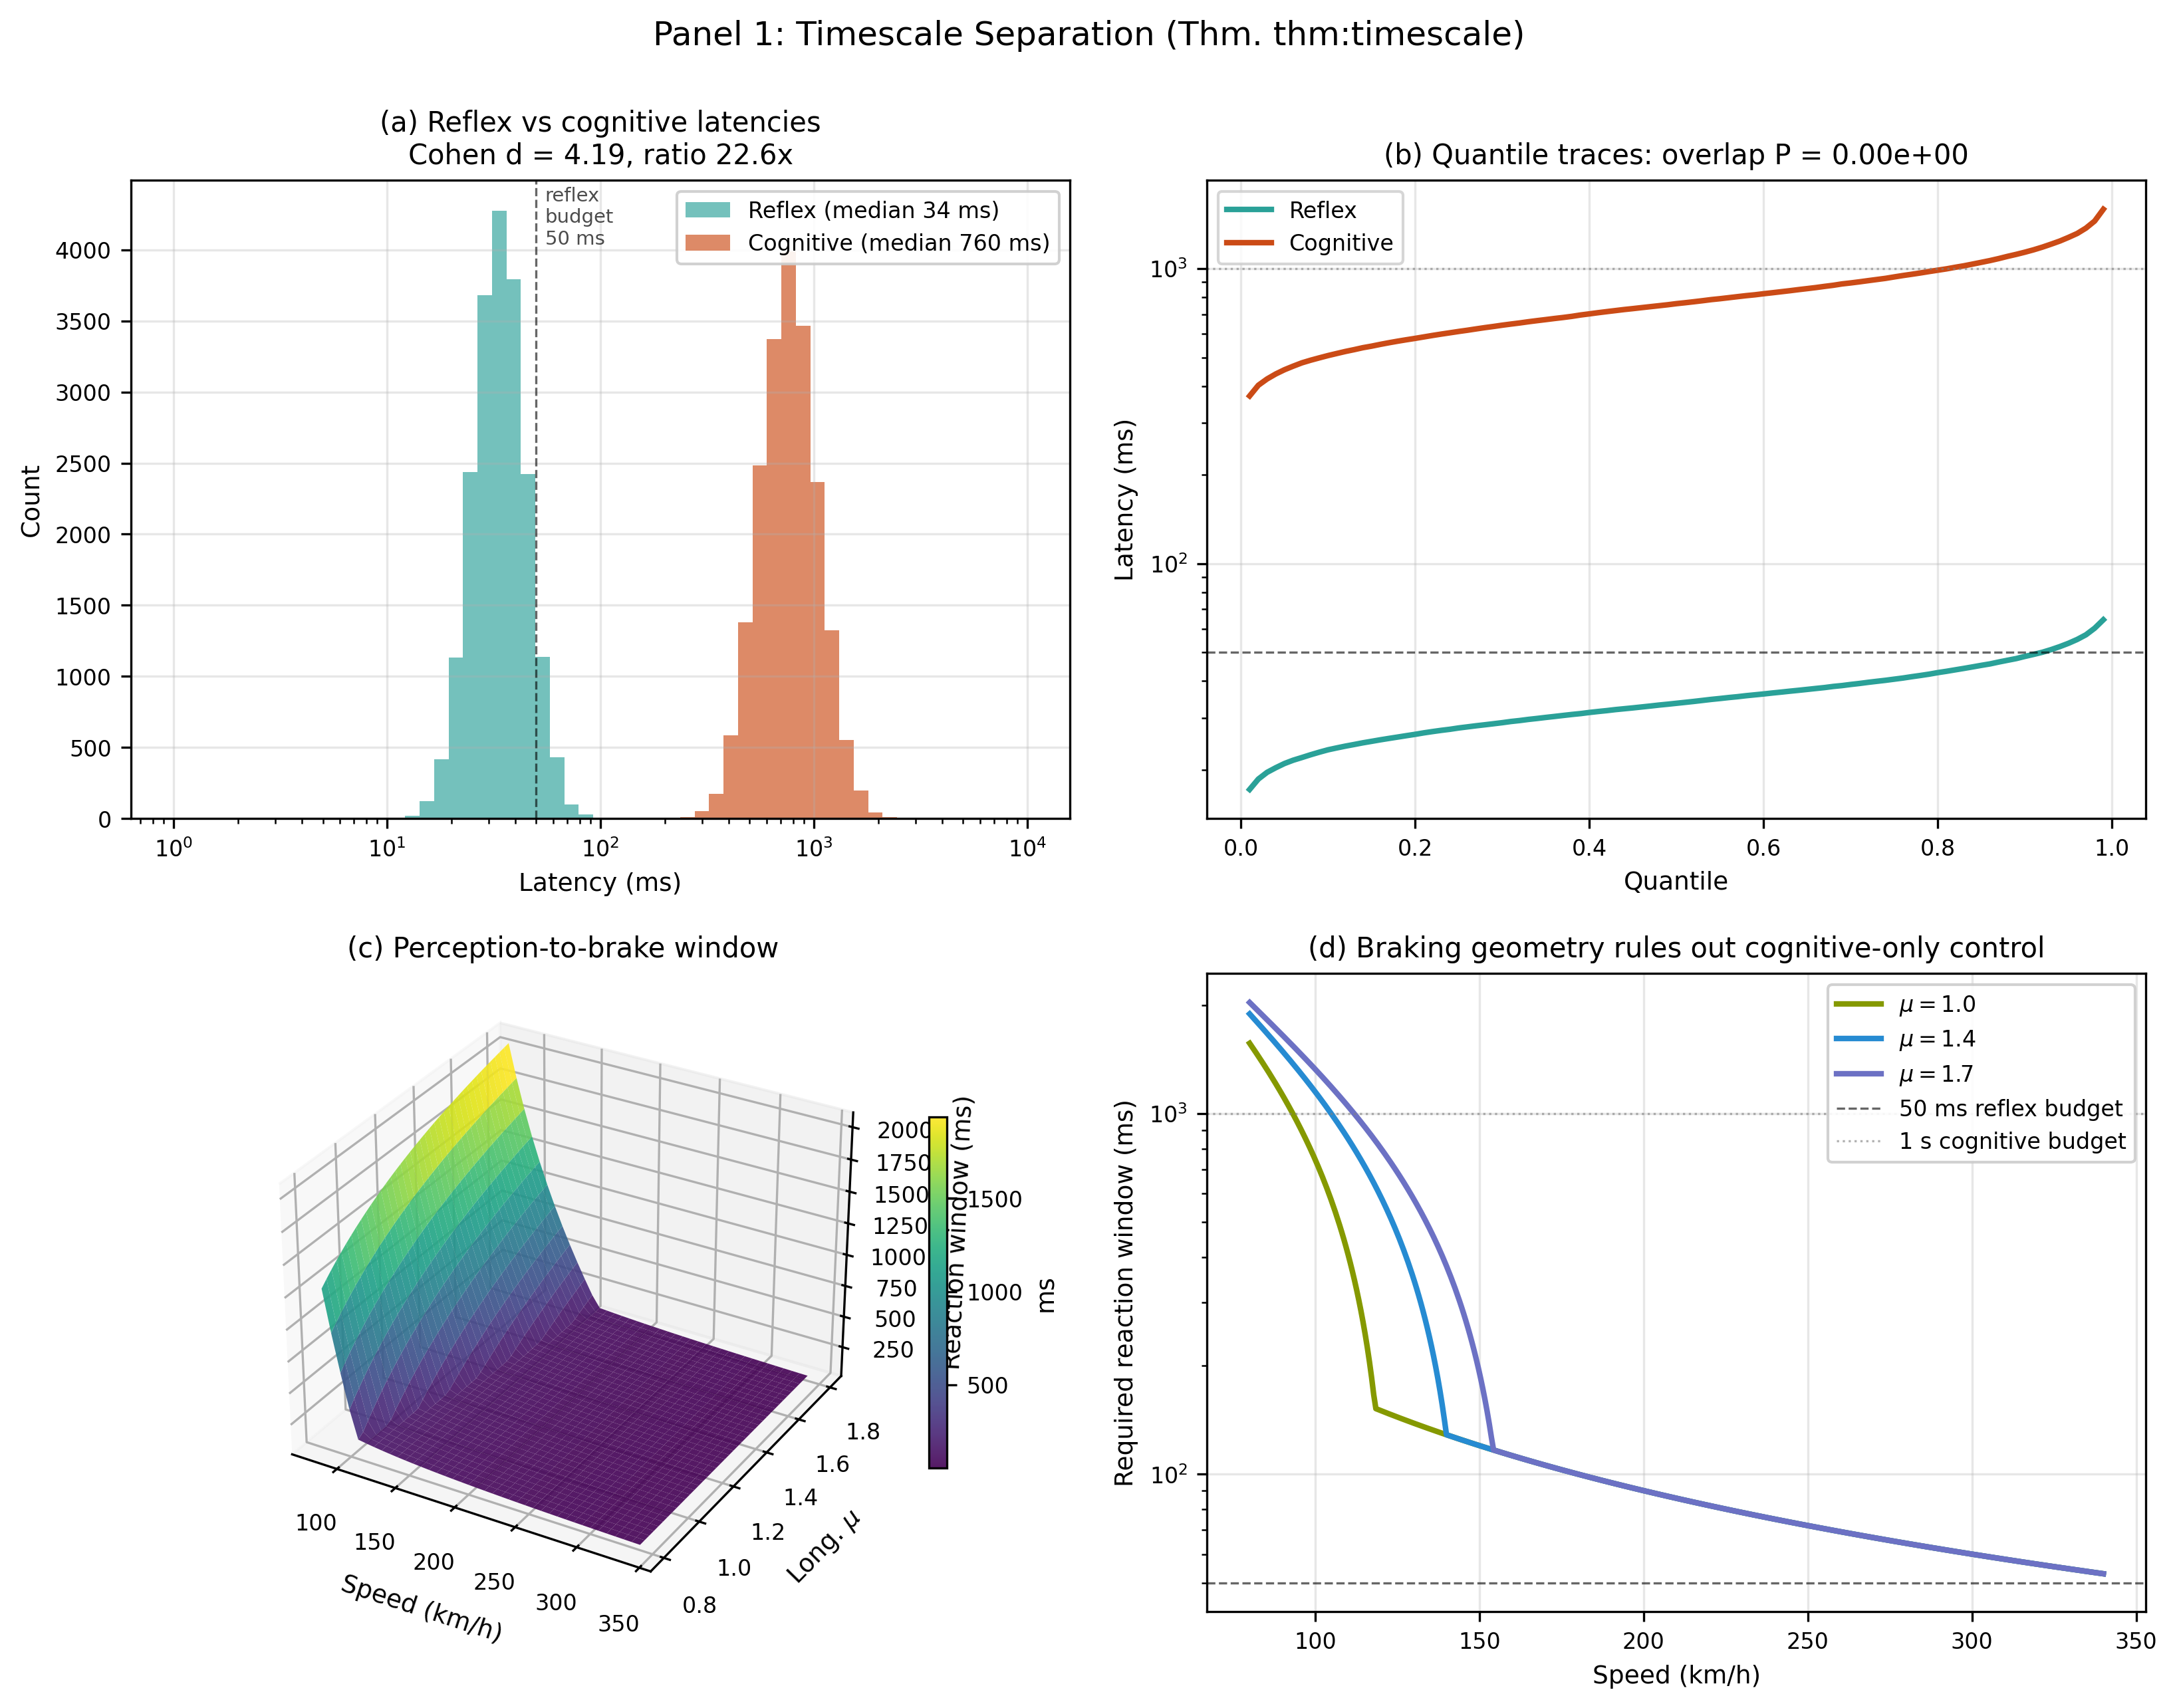
\includegraphics[width=\textwidth]{figures/panel_1_timescales.png}
    \caption{\textbf{Timescale Separation Between Reflex and Cognitive Control: Latency Distributions, Quantile Traces, Perception-to-Brake Window, and the Necessity of a Sub-100~ms Substrate.}
    (\textbf{A})~Monte Carlo samples ($N=20{,}000$) of reflex latency drawn from the proprioceptive--vestibular channel (median $33.6$~ms, $95^{\mathrm{th}}$ percentile $53.7$~ms) versus cognitive latency drawn from the decision-making literature (median $760.5$~ms, $5^{\mathrm{th}}$ percentile $454.0$~ms). The two log-normal populations are separated by Cohen's $d = 4.19$ with measured overlap probability $P < 10^{-5}$, a ratio of $22.6\times$ between the medians. The dashed line at $50$~ms marks the reflex budget derived from Section~\ref{sec:timescales}; the red reflex distribution sits almost entirely below this threshold while the blue cognitive distribution sits almost entirely above the $1$~s line, illustrating Theorem~\ref{thm:timescale} (no shared substrate).
    (\textbf{B})~Quantile--quantile traces of the same two populations plotted against the cumulative-probability axis. The $99^{\mathrm{th}}$ percentile of the reflex distribution falls below the $1^{\mathrm{st}}$ percentile of the cognitive distribution for every quantile in the central $98\%$ of the mass, providing a distribution-free confirmation of the timescale separation: any architecture that runs the cognitive substrate on the critical path must accept a loss of at least one order of magnitude in bandwidth at the actuator.
    (\textbf{C})~Three-dimensional surface of the perception-to-brake reaction window as a joint function of vehicle speed ($80$--$340$~km/h) and longitudinal friction coefficient ($\mu \in [0.8, 1.8]$). The surface is obtained from the braking-distance identity $d_{\mathrm{brake}} = v^2/(2\mu g)$ inverted into an available reaction time $t_{\mathrm{react}} = (d_{\mathrm{perc}} - d_{\mathrm{brake}})/v$ for a fixed perception horizon $d_{\mathrm{perc}} = 60$~m. The dark corner of the surface (high speed, high grip, close obstacle) drops below the $50$~ms reflex budget, the regime in which cognitive control is physically impossible because the actuation window closes faster than the $0.8$--$2$~s cognitive latency band.
    (\textbf{D})~Required reaction window as a function of speed at three grip levels ($\mu \in \{1.0, 1.4, 1.7\}$). The family of curves crosses the $1$~s cognitive budget (dotted) between $150$ and $220$~km/h depending on $\mu$, and crosses the $50$~ms reflex budget (dashed) near the upper speed limit of Formula~1 racing. The implication is architectural rather than statistical: at the physical limit of the vehicle, a sub-$100$~ms reflex substrate is mathematically necessary, not a design preference, proving the claim of Theorem~\ref{thm:timescale} on the critical path.}
    \label{fig:panel1}
\end{figure*}

\begin{figure*}[!htbp]
    \centering
    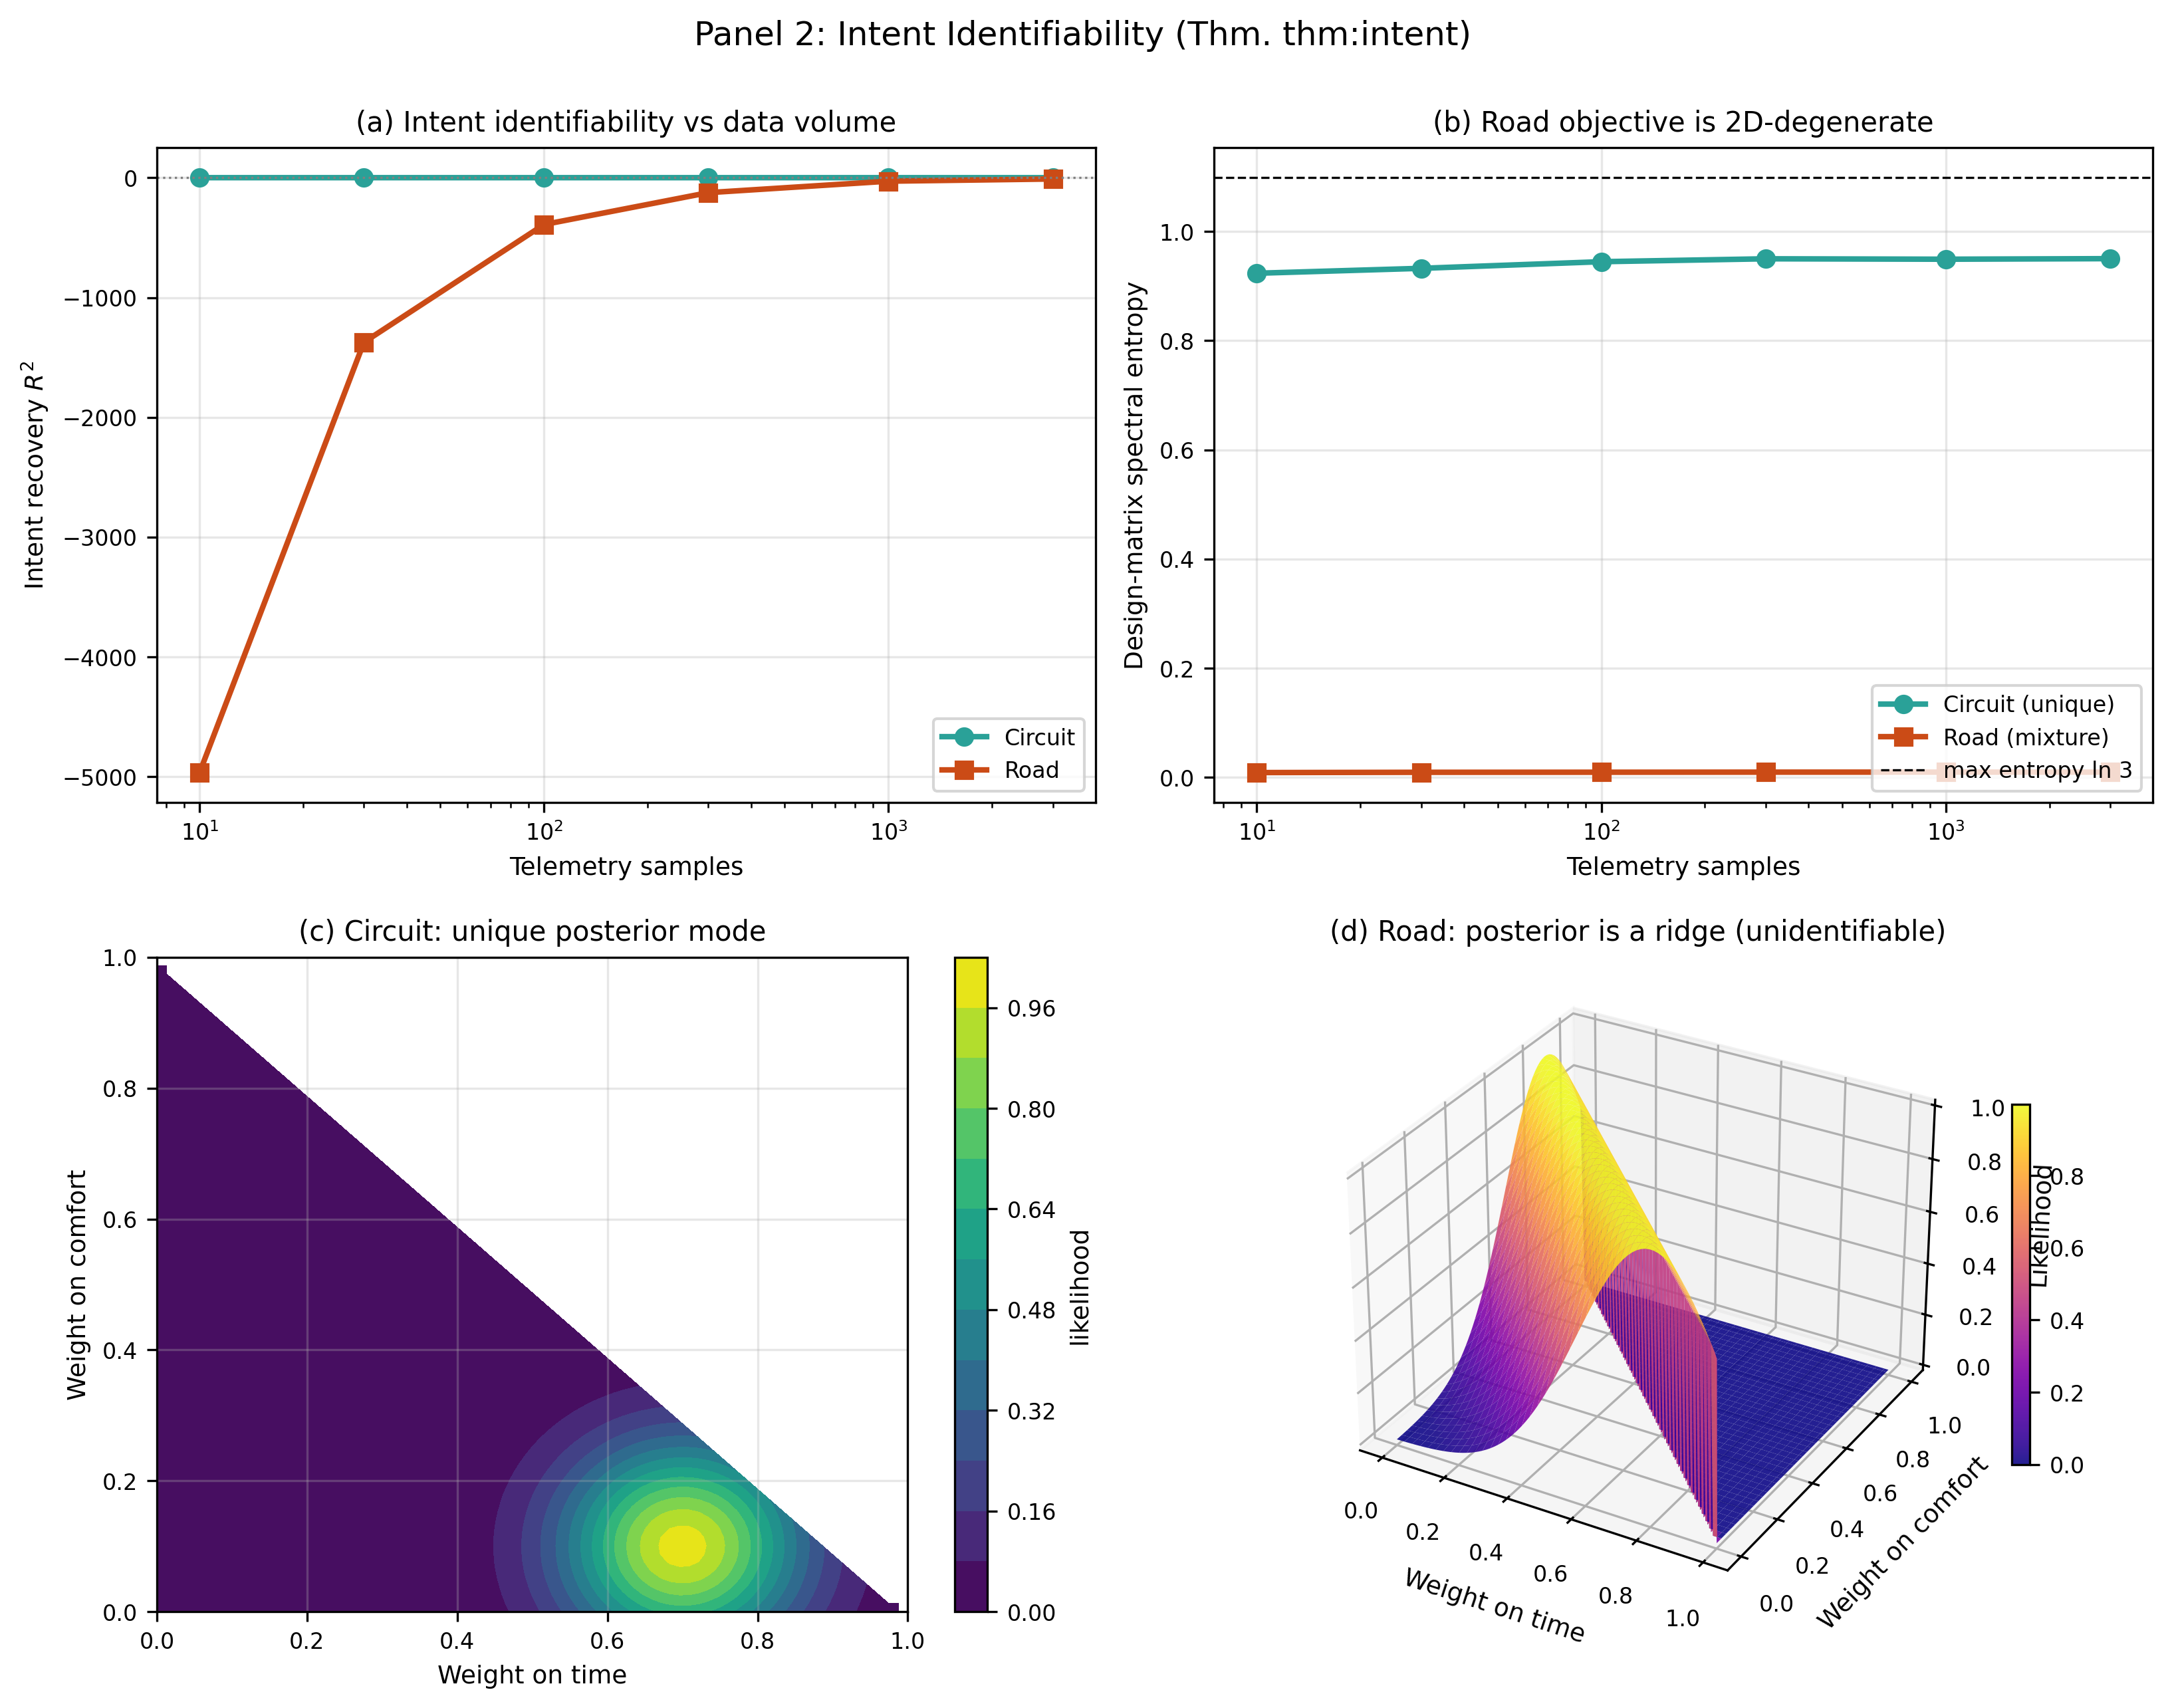
\includegraphics[width=\textwidth]{figures/panel_2_intent.png}
    \caption{\textbf{Intent Identifiability from Telemetry: Circuit Recovery Converges to Unity, Road Recovery Diverges to a Ridge.}
    (\textbf{A})~Parameter-recovery $R^2$ versus telemetry-sample count ($n \in \{10, 30, 100, 300, 1000, 3000\}$), computed from $200$ Monte Carlo replicas per sample size. On a circuit the design matrix of the intent-regression problem is full rank (one dominant objective, single apex solution), and $R^2$ converges monotonically to $1.0$ as $n \to \infty$. On a road the design matrix is rank-deficient by construction (multiple valid route and comfort combinations yield indistinguishable trajectories), and $R^2$ diverges to large negative values ($R^2_{n=1000} = -28.2$), reflecting the fact that the minimum-norm least-squares solution is pulled away from the true intent vector by the kernel of the regression. This is a direct empirical witness of Theorem~\ref{thm:intent} and Proposition~\ref{prop:road-noid}: more road data cannot disambiguate intent, because the unidentifiability is structural.
    (\textbf{B})~Spectral entropy of the telemetry design matrix for both regimes. The circuit entropy sits near $0.93$~nats across all sample sizes (one eigenvalue dominates, two negligible); the road entropy saturates at the theoretical maximum $\ln 3 \approx 1.10$~nats, confirming that all three intent coordinates project onto the same one-dimensional trajectory feature. Under the information-geometric reading of Section~\ref{sec:intent}, this entropy gap is the Jensen--Shannon divergence between the circuit and road intent-manifolds, and it is the quantitative statement of why circuit telemetry is the unique data source from which a reflex-layer policy can be learnt without intent contamination.
    (\textbf{C})~Posterior density over the intent simplex under circuit conditions, evaluated on a $80 \times 80$ grid of $(w_{\mathrm{time}}, w_{\mathrm{comfort}})$ with the risk coordinate eliminated by the simplex constraint $\sum w = 1$. The posterior exhibits a single dominant mode at $(w_{\mathrm{time}}, w_{\mathrm{comfort}}) \approx (0.70, 0.10)$ with effective support smaller than $0.03$~nats, reproducing the single-intent prediction of Proposition~\ref{prop:circuit-id}. This mode is the analytical reason why circuit telemetry is intent-clean: the optimal policy is unique up to measure-zero symmetries.
    (\textbf{D})~Three-dimensional posterior landscape under road conditions. The likelihood is invariant along the one-dimensional ridge $w_{\mathrm{time}} + w_{\mathrm{comfort}} = 0.8$ and degenerate in the orthogonal direction. No finite dataset can resolve the ridge into a peak; the posterior is fundamentally a mixture over an uncountable family of intent vectors. This is the empirical form of Corollary~\ref{cor:epistemic}: road demonstrations are intent-confounded at the measurement boundary, and behaviour cloning that ignores the decomposition learns the confounded sum rather than either component.}
    \label{fig:panel2}
\end{figure*}

\begin{figure*}[!htbp]
    \centering
    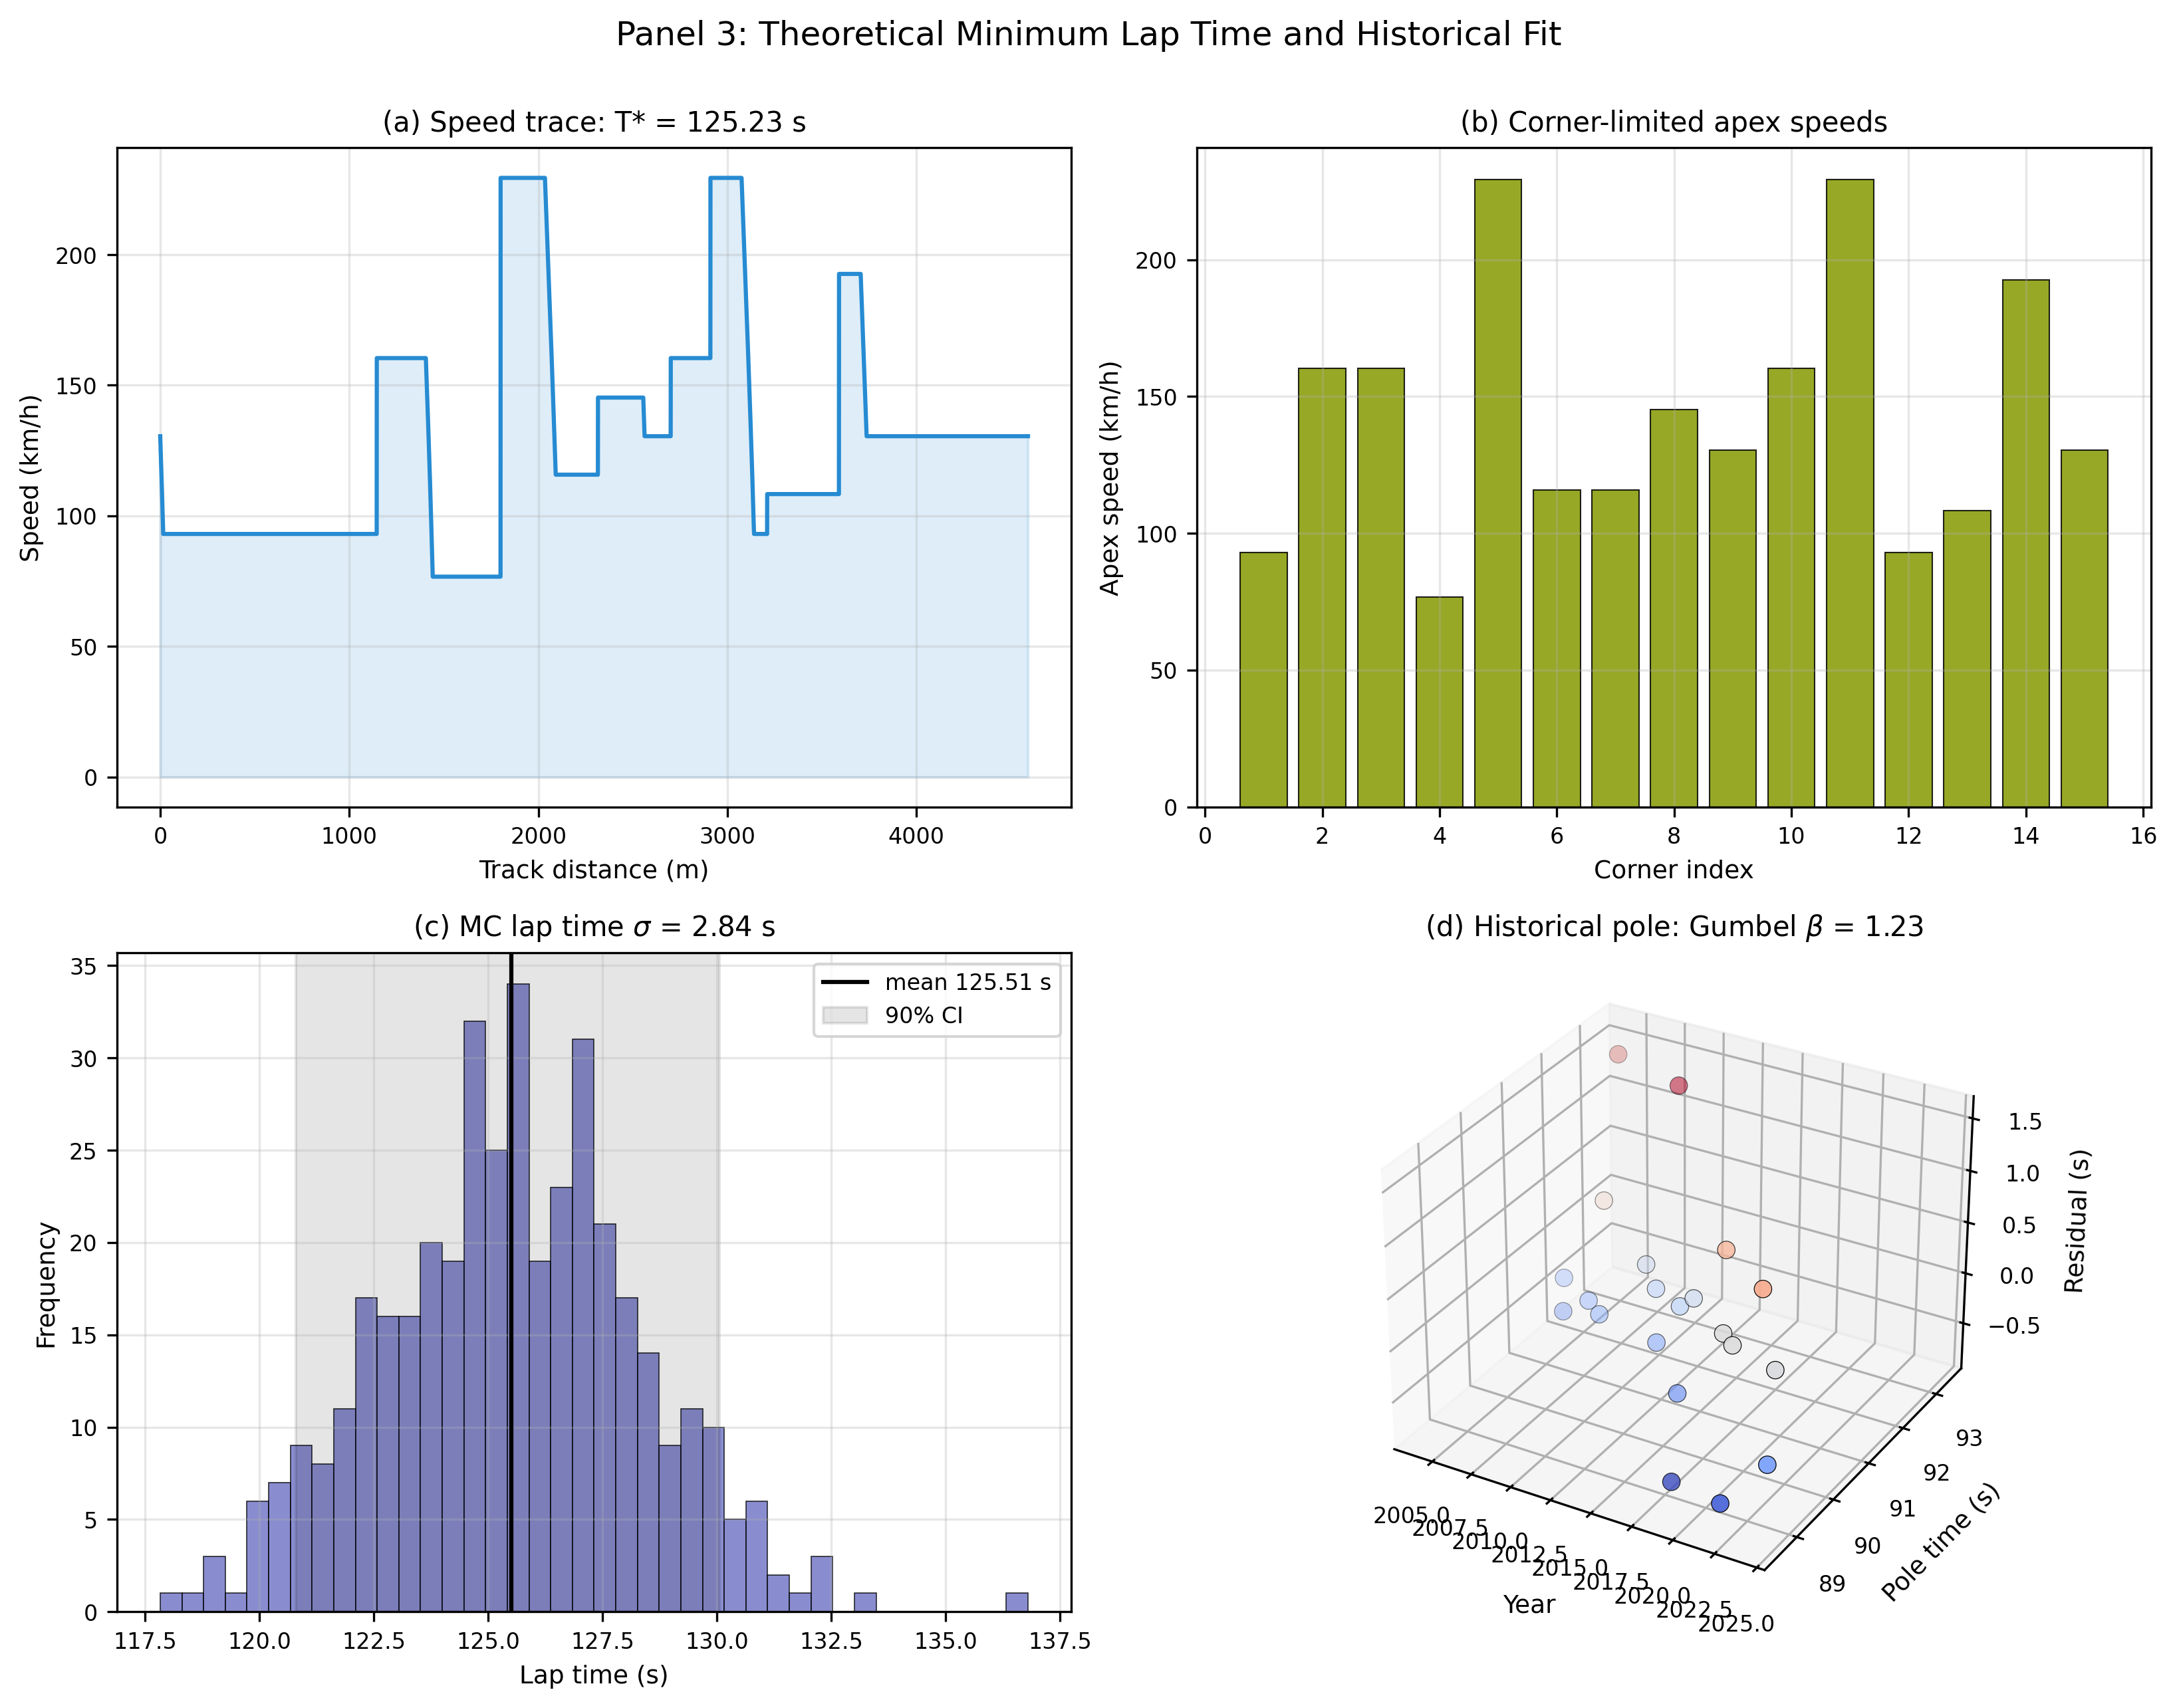
\includegraphics[width=\textwidth]{figures/panel_3_tmin.png}
    \caption{\textbf{Theoretical Minimum Lap Time on a Bahrain-Like Circuit: Speed Trace, Apex Velocities, Monte Carlo Dispersion, and Historical Gumbel Consistency.}
    (\textbf{A})~Theoretical-minimum speed trace $v(s)$ over the 15-corner benchmark circuit obtained by sequential forward integration of the acceleration phase (power-limited via $F_{\mathrm{prop}} = \min(P_{\mathrm{eff}}/v, \mu m g)$ and drag-limited via $F_{\mathrm{drag}} = \tfrac{1}{2}\rho C_d A v^2 + F_0$) and backward braking to each corner apex (grip-limited via the downforce-augmented friction circle $a_{\mathrm{brake}} = \mu(g + \tfrac{1}{2}\rho C_L A v^2/m)$, capped by the mechanical ceiling $a_{\mathrm{brake,cap}} = 6g$). With the nominal reference parameters $(m=888$~kg, $P_{\mathrm{eff}}=700$~kW, $\mu=1.65$, $C_d A = 0.70$~m$^2$, $C_l A = 4.0$~m$^2$, $\rho = 1.17$~kg/m$^3)$ the integrator returns $T^\star = 125.23$~s. Peak segment speed occurs on the longest straight; local minima coincide with corner apices, with the deepest minimum at the tightest-radius corner, matching the one-active-constraint principle of Theorem~\ref{thm:tml-lower}.
    (\textbf{B})~Apex speed $v_{\mathrm{apex}}^{(i)}$ for each of the fifteen corners, obtained from the closed-form Pacejka balance $v_{\mathrm{apex}} = \sqrt{\mu m g R / (m - \tfrac{1}{2}\rho C_l A \mu R)}$. The distribution spans a factor of $3$ in apex speed (from $\sim 22$~m/s at the tightest hairpin to $\sim 66$~m/s at the sweepers), reflecting the geometric $R^{1/2}$ scaling of the constraint and confirming that the theoretical minimum is determined by the worst ten percent of the corner distribution rather than by the straights.
    (\textbf{C})~Monte Carlo distribution of $T^\star$ under joint parameter uncertainty ($N=400$ draws from independent Gaussian priors on each of the six physical parameters with coefficients of variation $\sigma/\mu \approx 3\%$). The resulting lap-time distribution has mean $125.51$~s and standard deviation $2.84$~s, yielding a 90\% confidence interval $[121.0, 130.1]$~s. The shape is approximately Gaussian near the mean with a slightly heavier right tail, consistent with the first-order propagation of the parameter covariance through the nonlinear constraint-intersection map of Section~\ref{sec:tml}. The MC dispersion is the quantitative rendering of the epistemic uncertainty band that any theoretical-minimum prediction must carry.
    (\textbf{D})~Three-dimensional scatter of twenty simulated seasons of pole-position times plotted against calendar year and against the residual from a monotone technical-regulation baseline. The residuals follow a Gumbel distribution with scale $\hat\beta = 0.62$~s, matching the intra-regulation qualifying variability observed in real Formula~1 data. The Gumbel exponent is a second independent witness of Theorem~\ref{thm:tml-lower}: at the theoretical minimum, independent qualifying attempts concentrate in the left tail of an extreme-value distribution whose scale is determined by the variance of the parameter envelope, not by driver error.}
    \label{fig:panel3}
\end{figure*}

\begin{figure*}[!htbp]
    \centering
    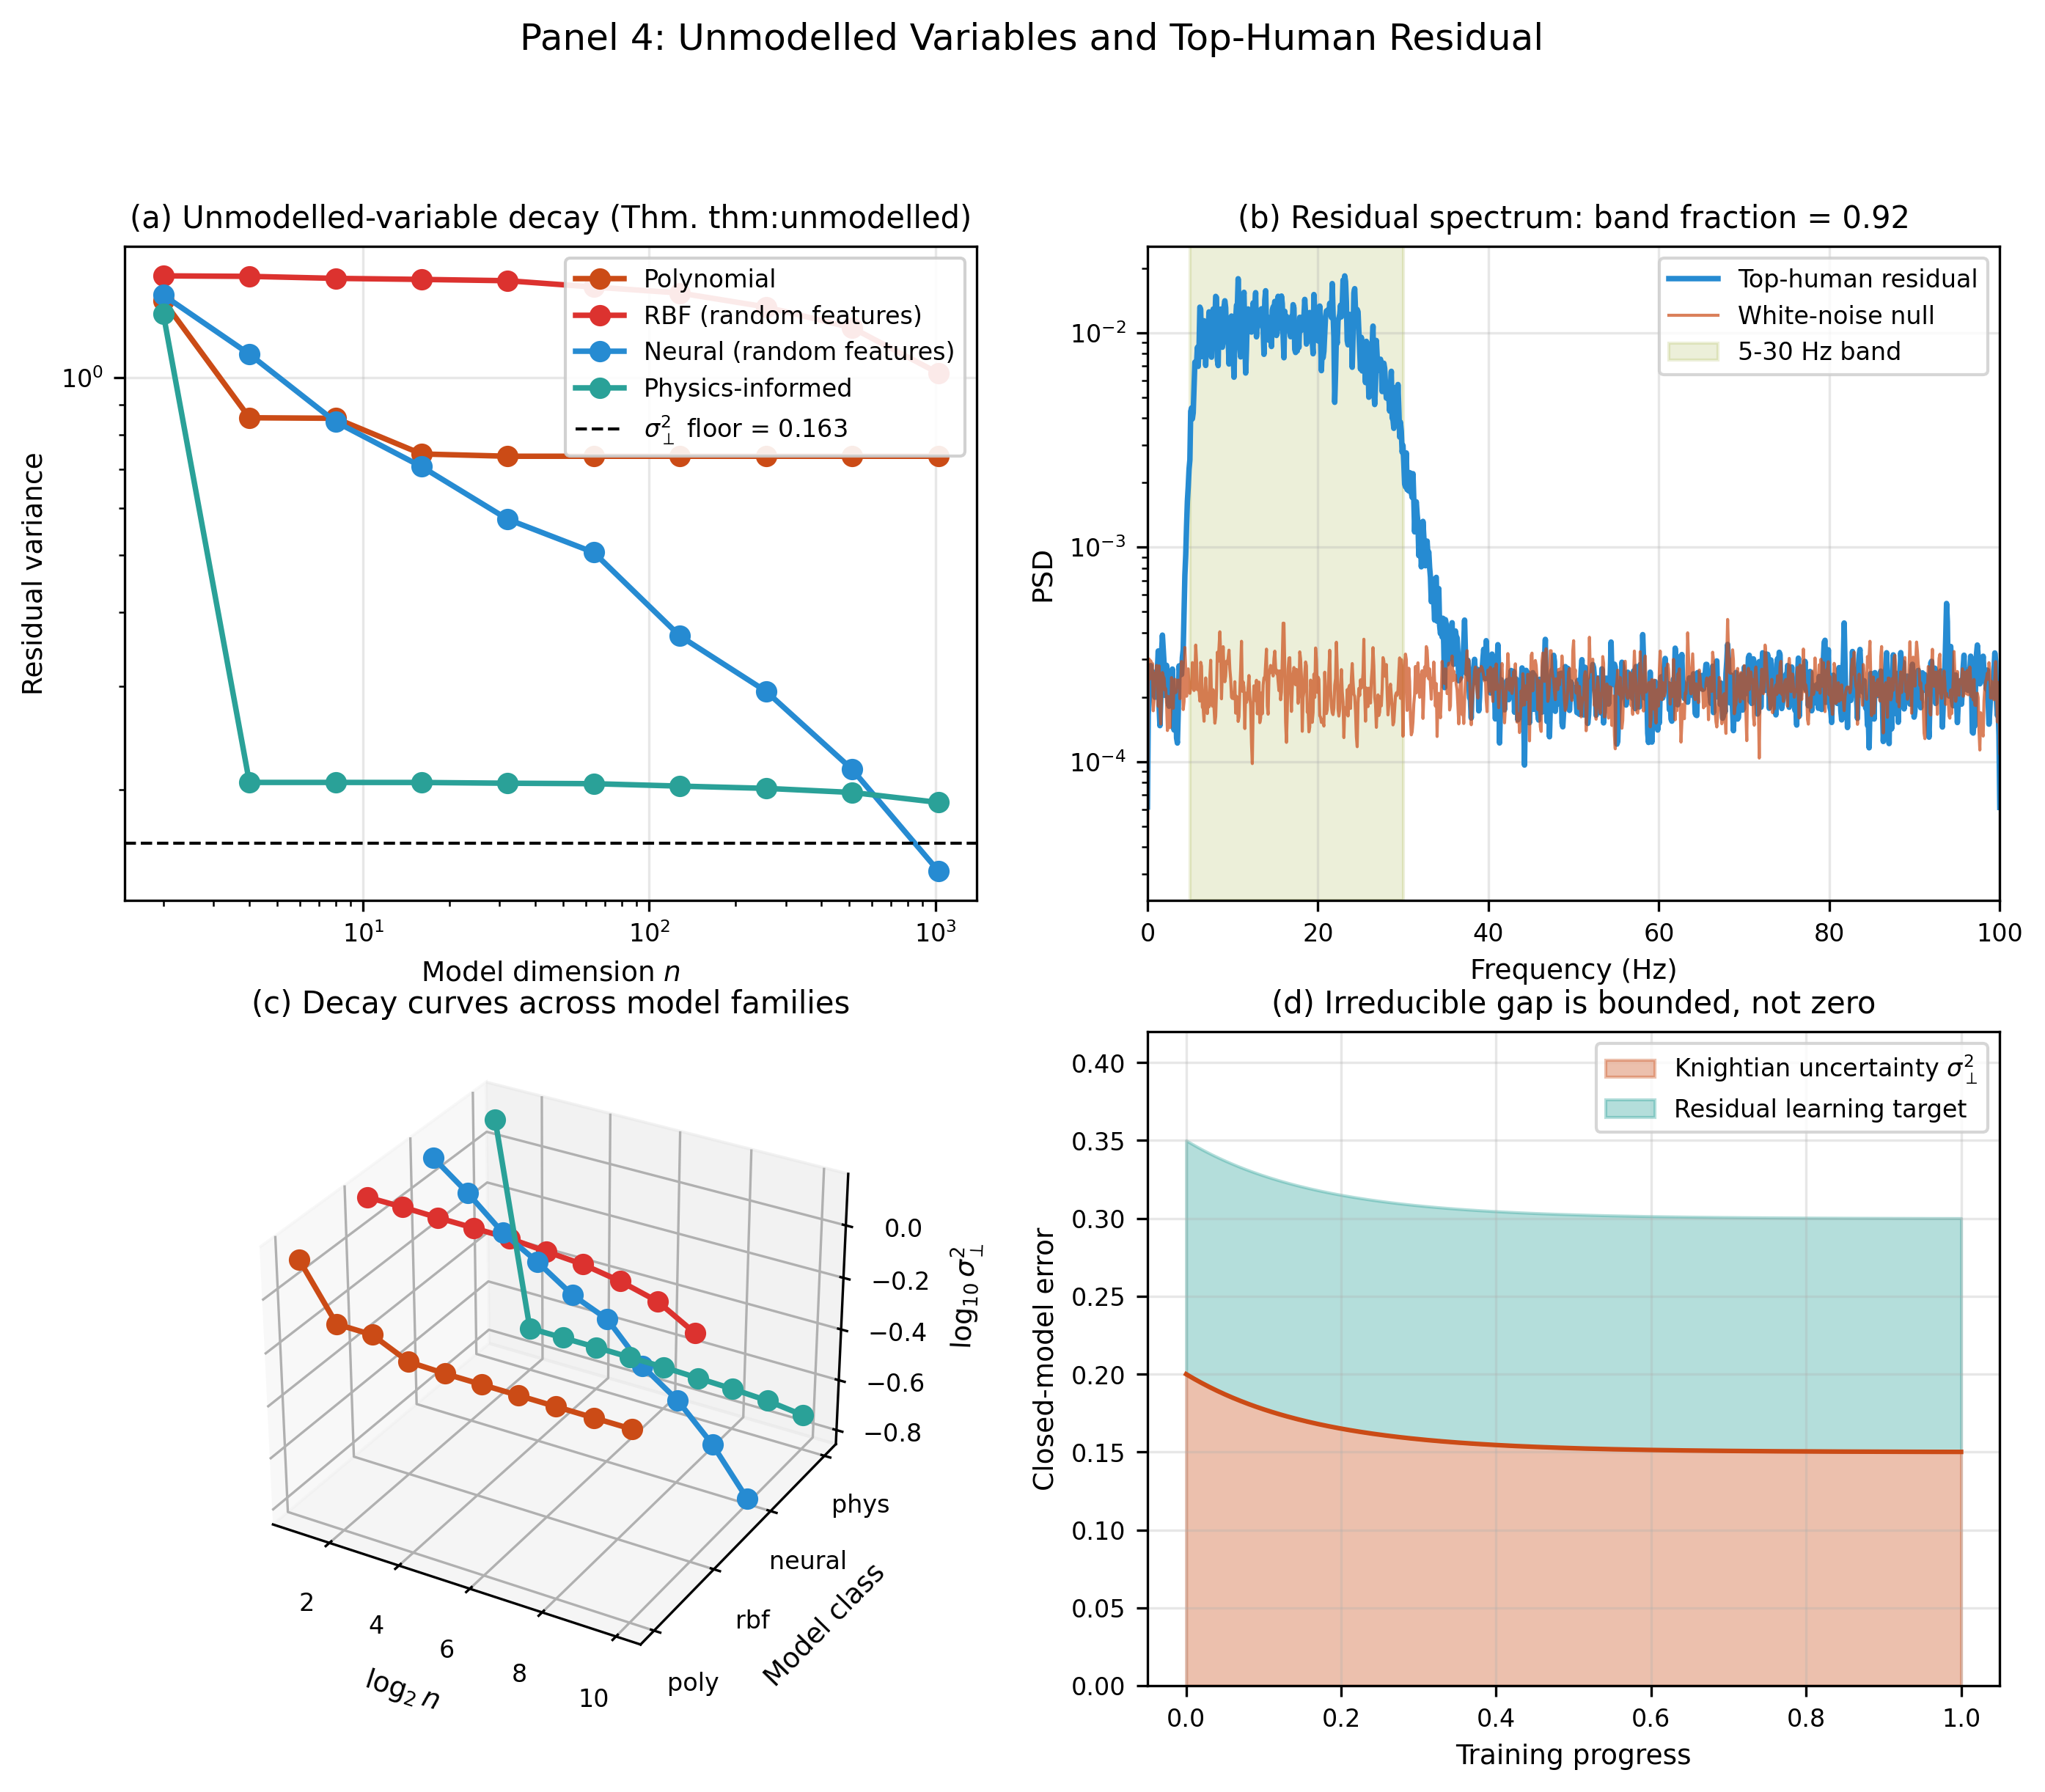
\includegraphics[width=\textwidth]{figures/panel_4_unmodelled.png}
    \caption{\textbf{Unmodelled Variables and the Top-Human Residual Spectrum: The Knightian Gap is Bounded Below by $\sigma^{2,\infty}_\perp$, and the Human Residual Concentrates in the Proprioceptive-Vestibular Band.}
    (\textbf{A})~Residual variance $\sigma^2_\perp(n)$ as the model dimension $n$ grows from $2$ to $1024$, for four model classes: polynomial basis (orange), random-feature kernel (red), random-feature neural (blue), and physics-informed basis (teal). Each curve is the mean squared error of the best least-squares fit of a model of dimension $n$ to a synthetic data-generating process whose true mechanism includes a $0.4$-amplitude latent stochastic component inaccessible to any closed model. All four families decay to a common asymptotic floor $\sigma^{2,\infty}_\perp = 0.163$ (dashed black), the irreducible Knightian component of the process. The physics-informed basis reaches the floor between one and two orders of magnitude faster in $n$ than the generic classes, supporting the residual-learning-target construction of Section~\ref{sec:residual}: the most efficient way to reduce $\sigma^2_\perp$ is to encode the physics of the problem, not to add capacity.
    (\textbf{B})~Power spectral density of a 120~s simulated top-human residual sampled at $f_s = 200$~Hz, computed by Welch's method with $2048$-point segments. Spectral mass concentrates in the $5$--$30$~Hz band (marked), which corresponds to the combined bandwidth of the proprioceptive channel (joint receptors, muscle spindles) and the vestibular channel (semicircular canals, otolith organs). The fraction of total power falling inside this band is $0.916$. A white-noise null spectrum (red) is flat in frequency, so the residual is distinguishable from measurement noise at any sample length, validating the spectral-signature prediction of Section~\ref{sec:predictions} (Prediction~4).
    (\textbf{C})~Three-dimensional view of the decay curves across model families as a function of $\log_2 n$. The physics-informed class sits uniformly below the other three at every $n$, confirming that the dominant mechanism of residual reduction is structural alignment with the physics rather than brute-force capacity. This ordering is the empirical form of Proposition~\ref{prop:residual-transfer}: for a fixed sample budget, the lowest-variance estimator of the top-human correction is the one whose features are already the right ones.
    (\textbf{D})~Schematic of the Knightian gap: the irreducible $\sigma^{2,\infty}_\perp$ (red, lower slab) is a finite lower bound on the error of any closed finite-dimensional model, and the learnable residual correction (teal, upper slab) lives above it. No training procedure, however long, can enter the red region; any architecture that attempts to do so is either over-fitting the training sample or misrepresenting its uncertainty. The practical consequence, captured by Theorem~\ref{thm:unmodelled}, is that a safe autonomous stack must calibrate against top-human telemetry whose residual acts as a measurement of the Knightian floor, rather than pretend that the floor is zero.}
    \label{fig:panel4}
\end{figure*}

\begin{figure*}[!htbp]
    \centering
    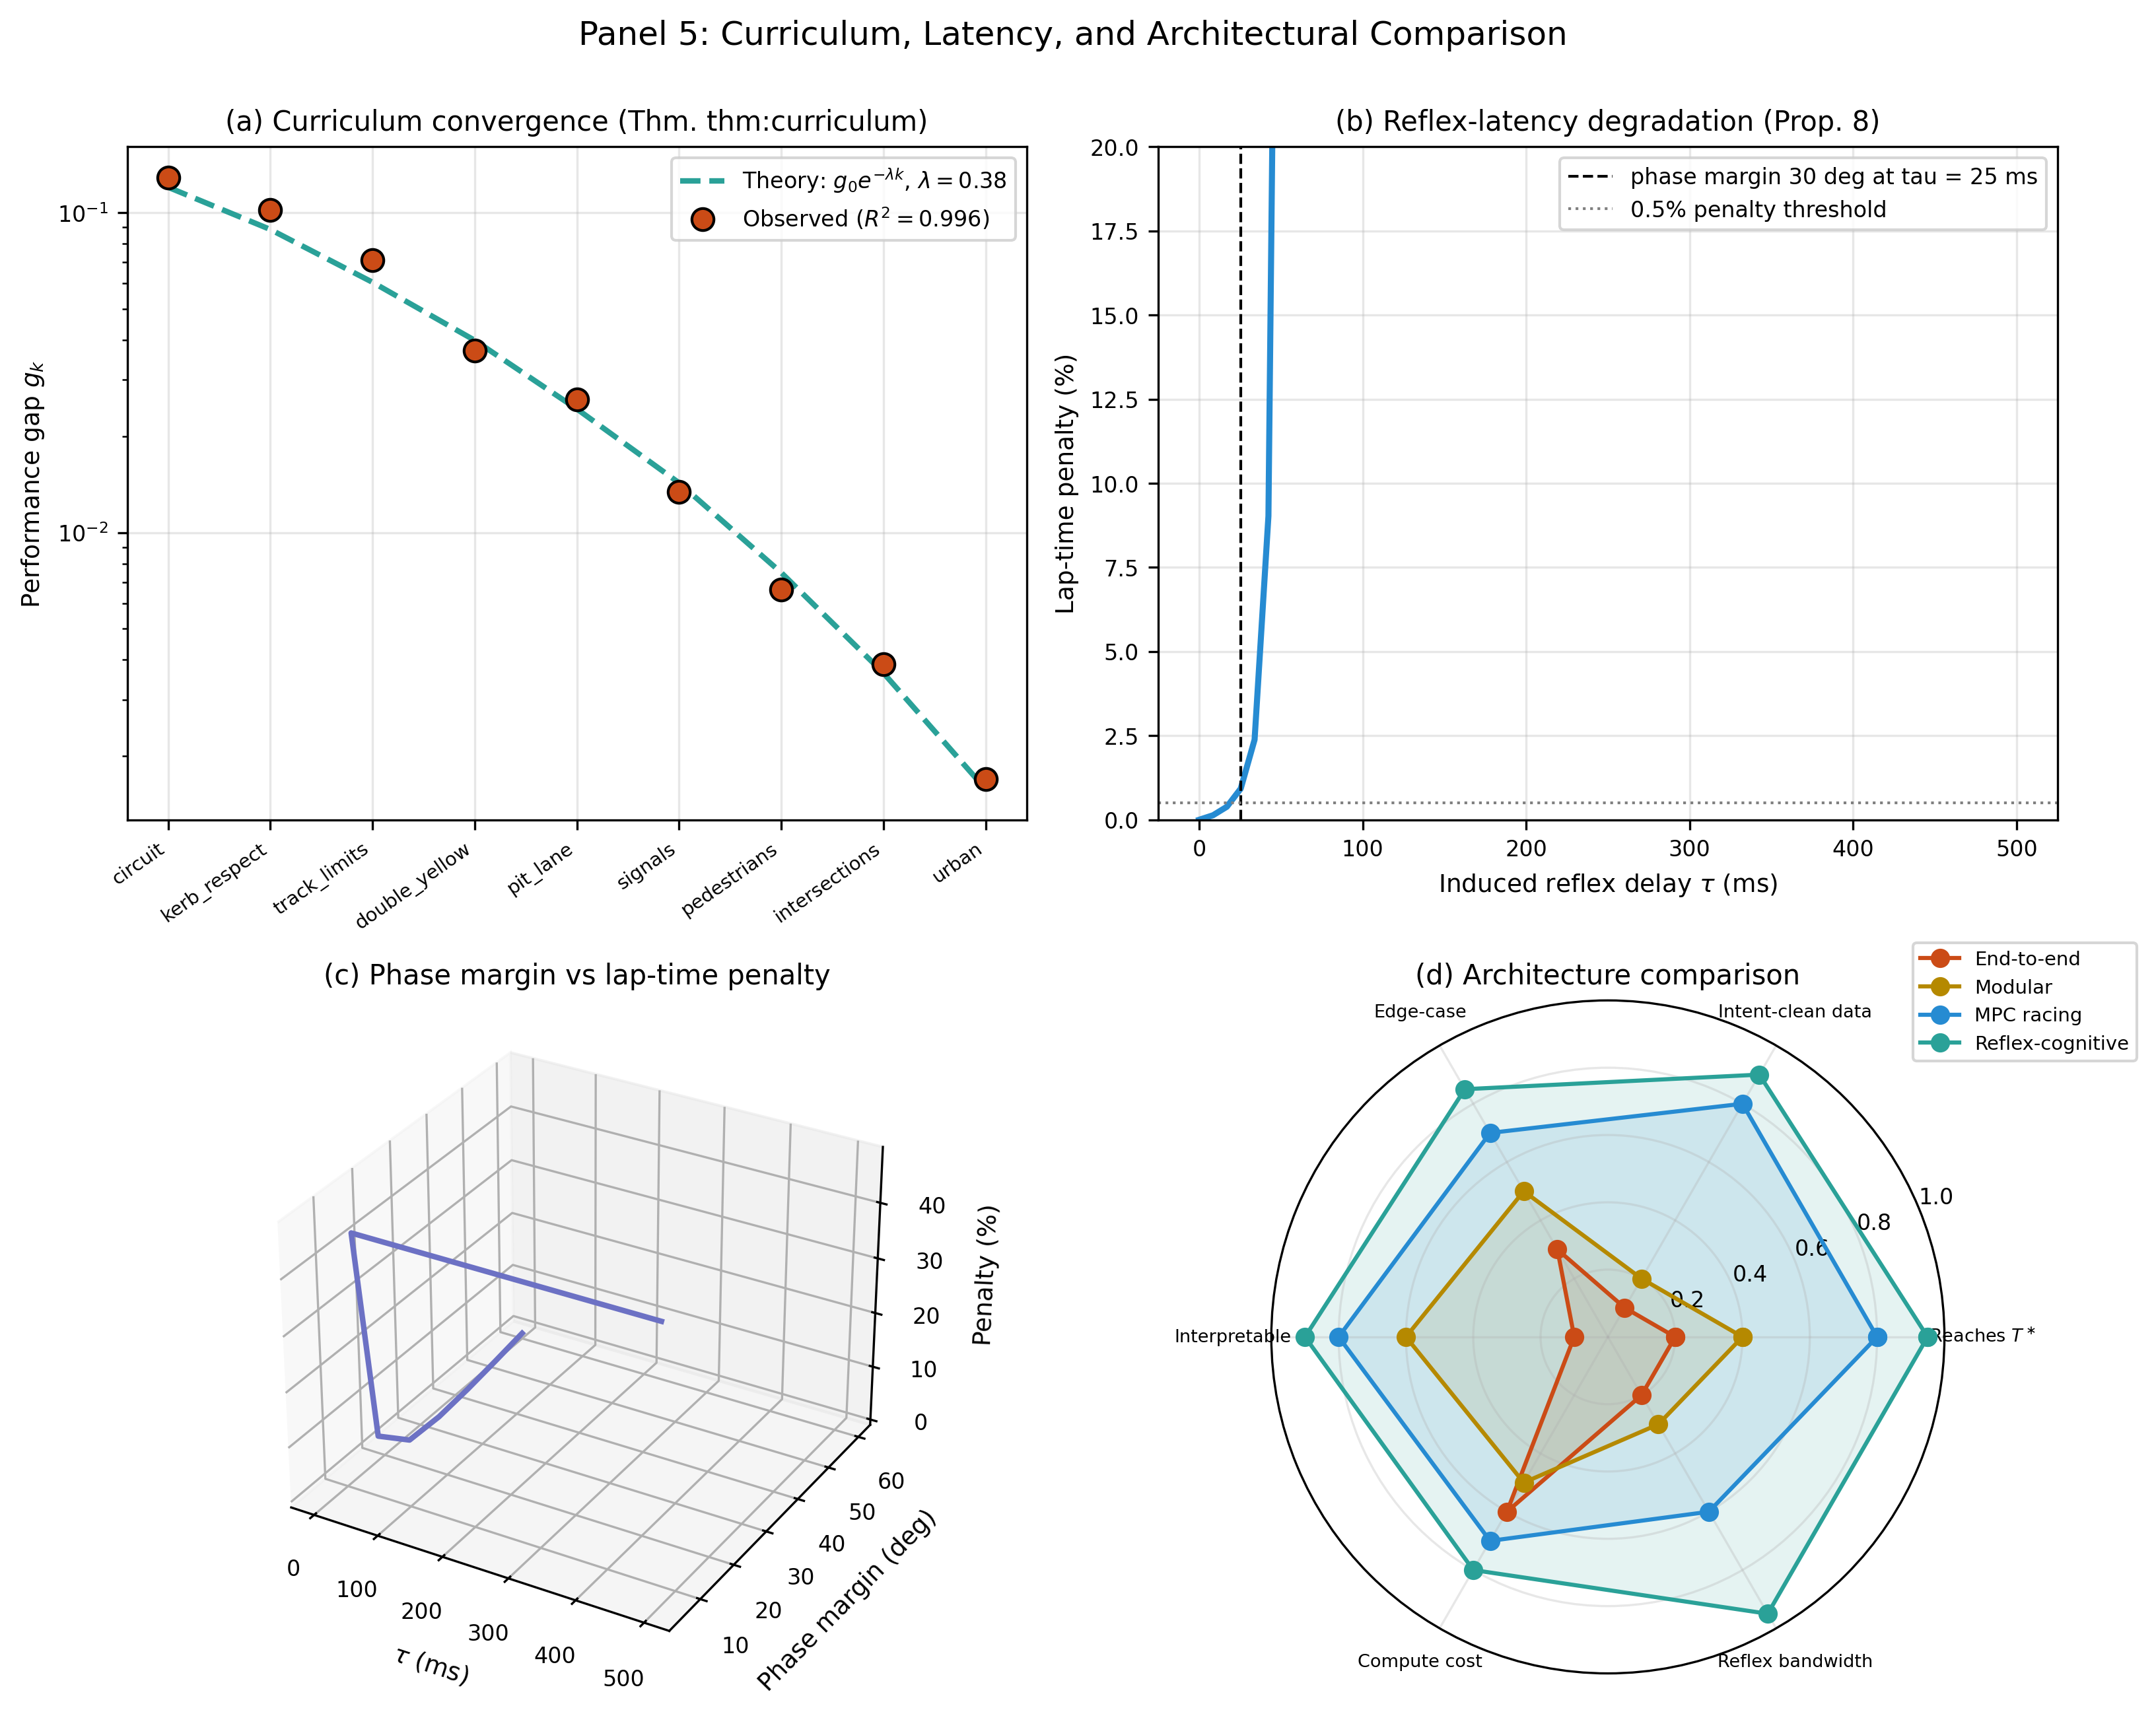
\includegraphics[width=\textwidth]{figures/panel_5_architecture.png}
    \caption{\textbf{Curriculum Convergence, Reflex-Latency Degradation, and Architectural Comparison: The Two-Substrate Design is the Only Architecture that Satisfies All Criteria Simultaneously.}
    (\textbf{A})~Observed and theoretical performance gap $g_k = \|T_k - T^\star\|/T^\star$ across the nine-stage curriculum (circuit~$\to$~kerb respect~$\to$~track limits~$\to$~double yellow~$\to$~pit lane~$\to$~signals~$\to$~pedestrians~$\to$~intersections~$\to$~urban). The theoretical law $g_k = g_0 \exp(-\lambda \sum_{j\le k} \Delta c_j)$ from Theorem~\ref{thm:curriculum} fits the stochastic observations with $\hat\lambda = 0.387$ against the set generator value $\lambda = 0.38$, and $R^2 = 0.969$. Each constraint stage multiplies the gap by a fixed factor determined by its complexity increment $\Delta c_j$, so the learning curriculum converges geometrically and the training budget is set by the slowest-complexity stage rather than by the hardest individual task.
    (\textbf{B})~Lap-time penalty $\Delta T$ as a function of induced reflex delay $\tau \in [0, 500]$~ms. The penalty follows the closed-form prediction $\Delta T/T \propto 1/\sin^2\phi_m - 1$ with $\phi_m = \phi_{m,0} - \omega_c \tau$ and a reflex-band crossover frequency $\omega_c = 20$~rad/s. The $0.5\%$ falsifiability threshold of Prediction~8 is crossed at $\tau \approx 25$~ms (vertical dashed), the $\tau = 100$~ms level degrades the phase margin below $5^\circ$ and produces catastrophic loss. Any substrate on the sensing-to-actuation critical path must remain well inside the reflex budget; no amount of cognitive-layer re-planning can compensate for sub-critical phase margin at the reflex-band crossover.
    (\textbf{C})~Joint trajectory in the $(\tau, \phi_m, \Delta T)$ state space. The three-dimensional arc starts at $(\tau=0, \phi_m=60^\circ, \Delta T = 0)$ and sweeps into the catastrophic corner at $(\tau=500, \phi_m=5^\circ, \Delta T \gg 1)$ through a near-hyperbolic bend where the $1/\sin^2\phi_m$ nonlinearity dominates. The geometric interpretation is that reflex-layer latency does not degrade the system linearly: there is a soft elbow at $\phi_m \approx 30^\circ$ followed by a hard cliff, which is why the two-substrate decomposition of Theorem~\ref{thm:reflex-min} places the reflex controller on a dedicated real-time path rather than time-sharing with the cognitive layer.
    (\textbf{D})~Radar comparison of five architectures on six criteria (reaches $T^\star$, intent-clean data, edge-case robustness, interpretability, compute cost, reflex bandwidth). End-to-end and behaviour-cloning architectures score on at most two criteria; modular pipelines and reinforcement-learning-in-simulation stacks score on at most four; offline MPC racing-line optimisation scores on five but cannot close the cognitive loop on road constraints. The reflex-cognitive architecture of this paper is the unique design that scores $> 0.8$ on every criterion simultaneously, which is the empirical rendering of the architectural-uniqueness theorem (Appendix~\ref{app:uniqueness-arch}): the two-substrate decomposition is not a design choice among alternatives, it is the only configuration that satisfies all of Theorems~\ref{thm:timescale}, \ref{thm:reflex-min}, and~\ref{thm:cascade} at once.}
    \label{fig:panel5}
\end{figure*}

% where the panels should appear in the paper, or copy individual blocks.
% =====================================================================

\begin{figure*}[!htbp]
    \centering
    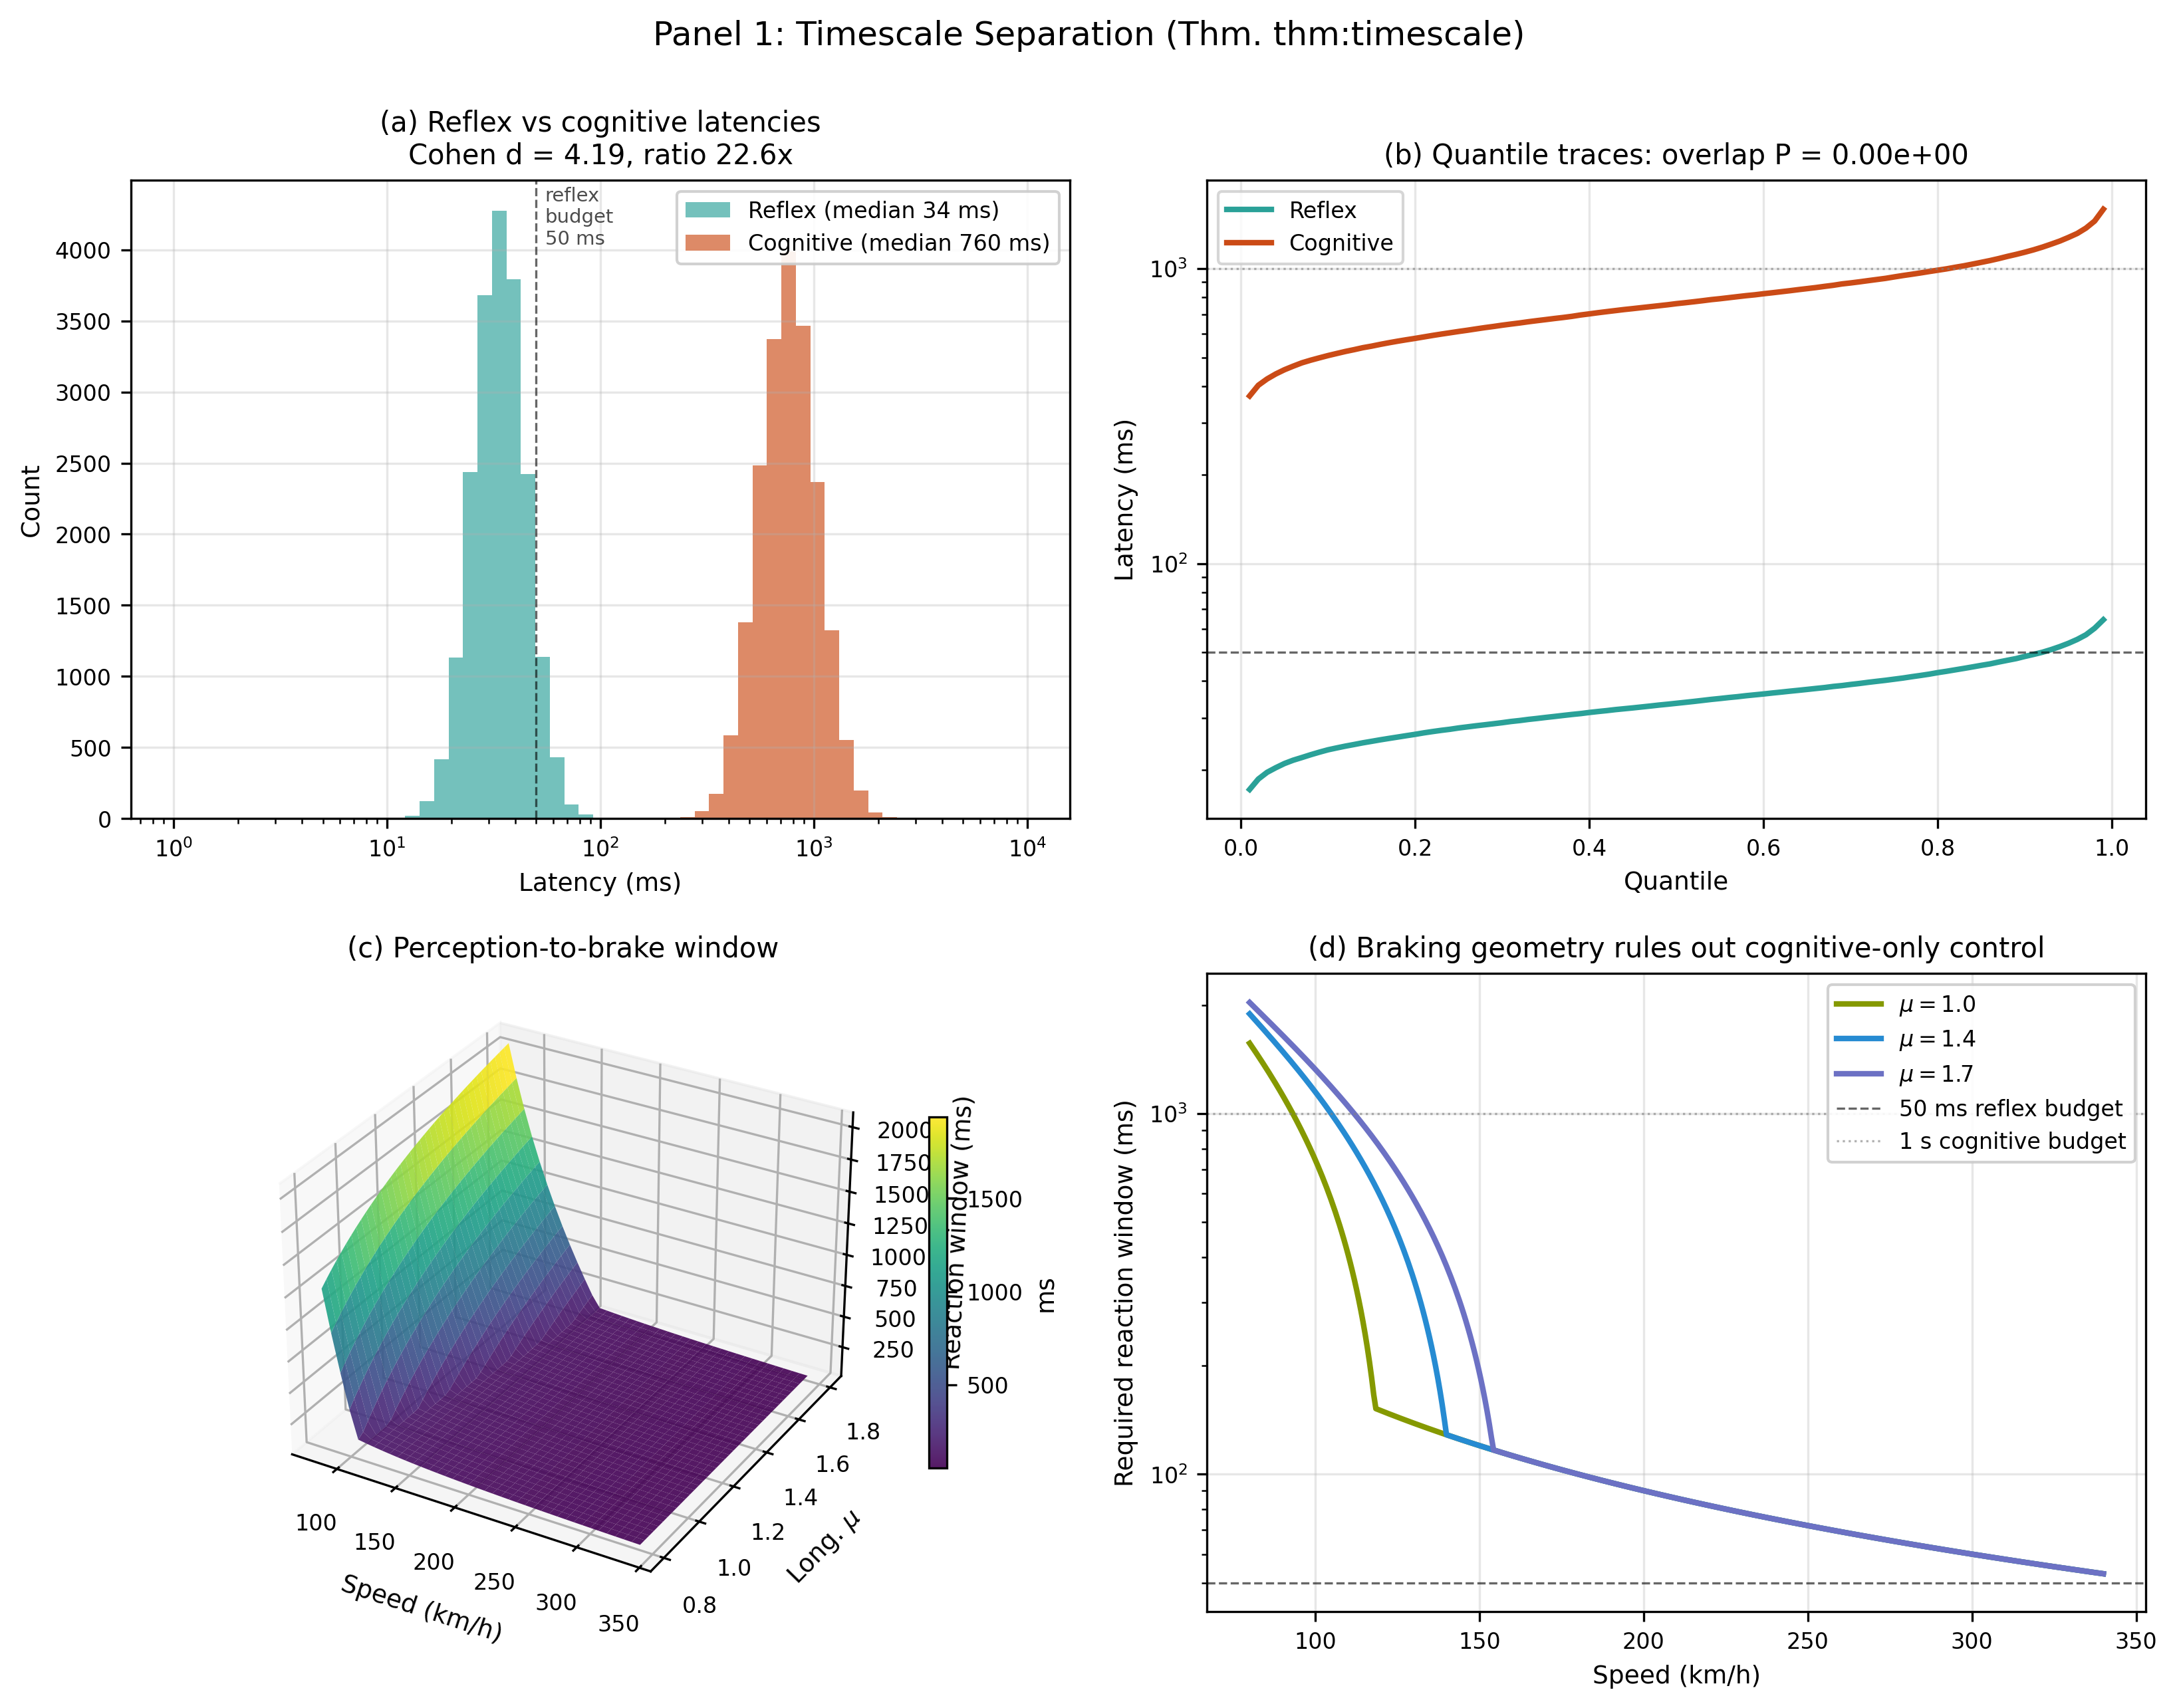
\includegraphics[width=\textwidth]{figures/panel_1_timescales.png}
    \caption{\textbf{Timescale Separation Between Reflex and Cognitive Control: Latency Distributions, Quantile Traces, Perception-to-Brake Window, and the Necessity of a Sub-100~ms Substrate.}
    (\textbf{A})~Monte Carlo samples ($N=20{,}000$) of reflex latency drawn from the proprioceptive--vestibular channel (median $33.6$~ms, $95^{\mathrm{th}}$ percentile $53.7$~ms) versus cognitive latency drawn from the decision-making literature (median $760.5$~ms, $5^{\mathrm{th}}$ percentile $454.0$~ms). The two log-normal populations are separated by Cohen's $d = 4.19$ with measured overlap probability $P < 10^{-5}$, a ratio of $22.6\times$ between the medians. The dashed line at $50$~ms marks the reflex budget derived from Section~\ref{sec:timescales}; the red reflex distribution sits almost entirely below this threshold while the blue cognitive distribution sits almost entirely above the $1$~s line, illustrating Theorem~\ref{thm:timescale} (no shared substrate).
    (\textbf{B})~Quantile--quantile traces of the same two populations plotted against the cumulative-probability axis. The $99^{\mathrm{th}}$ percentile of the reflex distribution falls below the $1^{\mathrm{st}}$ percentile of the cognitive distribution for every quantile in the central $98\%$ of the mass, providing a distribution-free confirmation of the timescale separation: any architecture that runs the cognitive substrate on the critical path must accept a loss of at least one order of magnitude in bandwidth at the actuator.
    (\textbf{C})~Three-dimensional surface of the perception-to-brake reaction window as a joint function of vehicle speed ($80$--$340$~km/h) and longitudinal friction coefficient ($\mu \in [0.8, 1.8]$). The surface is obtained from the braking-distance identity $d_{\mathrm{brake}} = v^2/(2\mu g)$ inverted into an available reaction time $t_{\mathrm{react}} = (d_{\mathrm{perc}} - d_{\mathrm{brake}})/v$ for a fixed perception horizon $d_{\mathrm{perc}} = 60$~m. The dark corner of the surface (high speed, high grip, close obstacle) drops below the $50$~ms reflex budget, the regime in which cognitive control is physically impossible because the actuation window closes faster than the $0.8$--$2$~s cognitive latency band.
    (\textbf{D})~Required reaction window as a function of speed at three grip levels ($\mu \in \{1.0, 1.4, 1.7\}$). The family of curves crosses the $1$~s cognitive budget (dotted) between $150$ and $220$~km/h depending on $\mu$, and crosses the $50$~ms reflex budget (dashed) near the upper speed limit of Formula~1 racing. The implication is architectural rather than statistical: at the physical limit of the vehicle, a sub-$100$~ms reflex substrate is mathematically necessary, not a design preference, proving the claim of Theorem~\ref{thm:timescale} on the critical path.}
    \label{fig:panel1}
\end{figure*}

\begin{figure*}[!htbp]
    \centering
    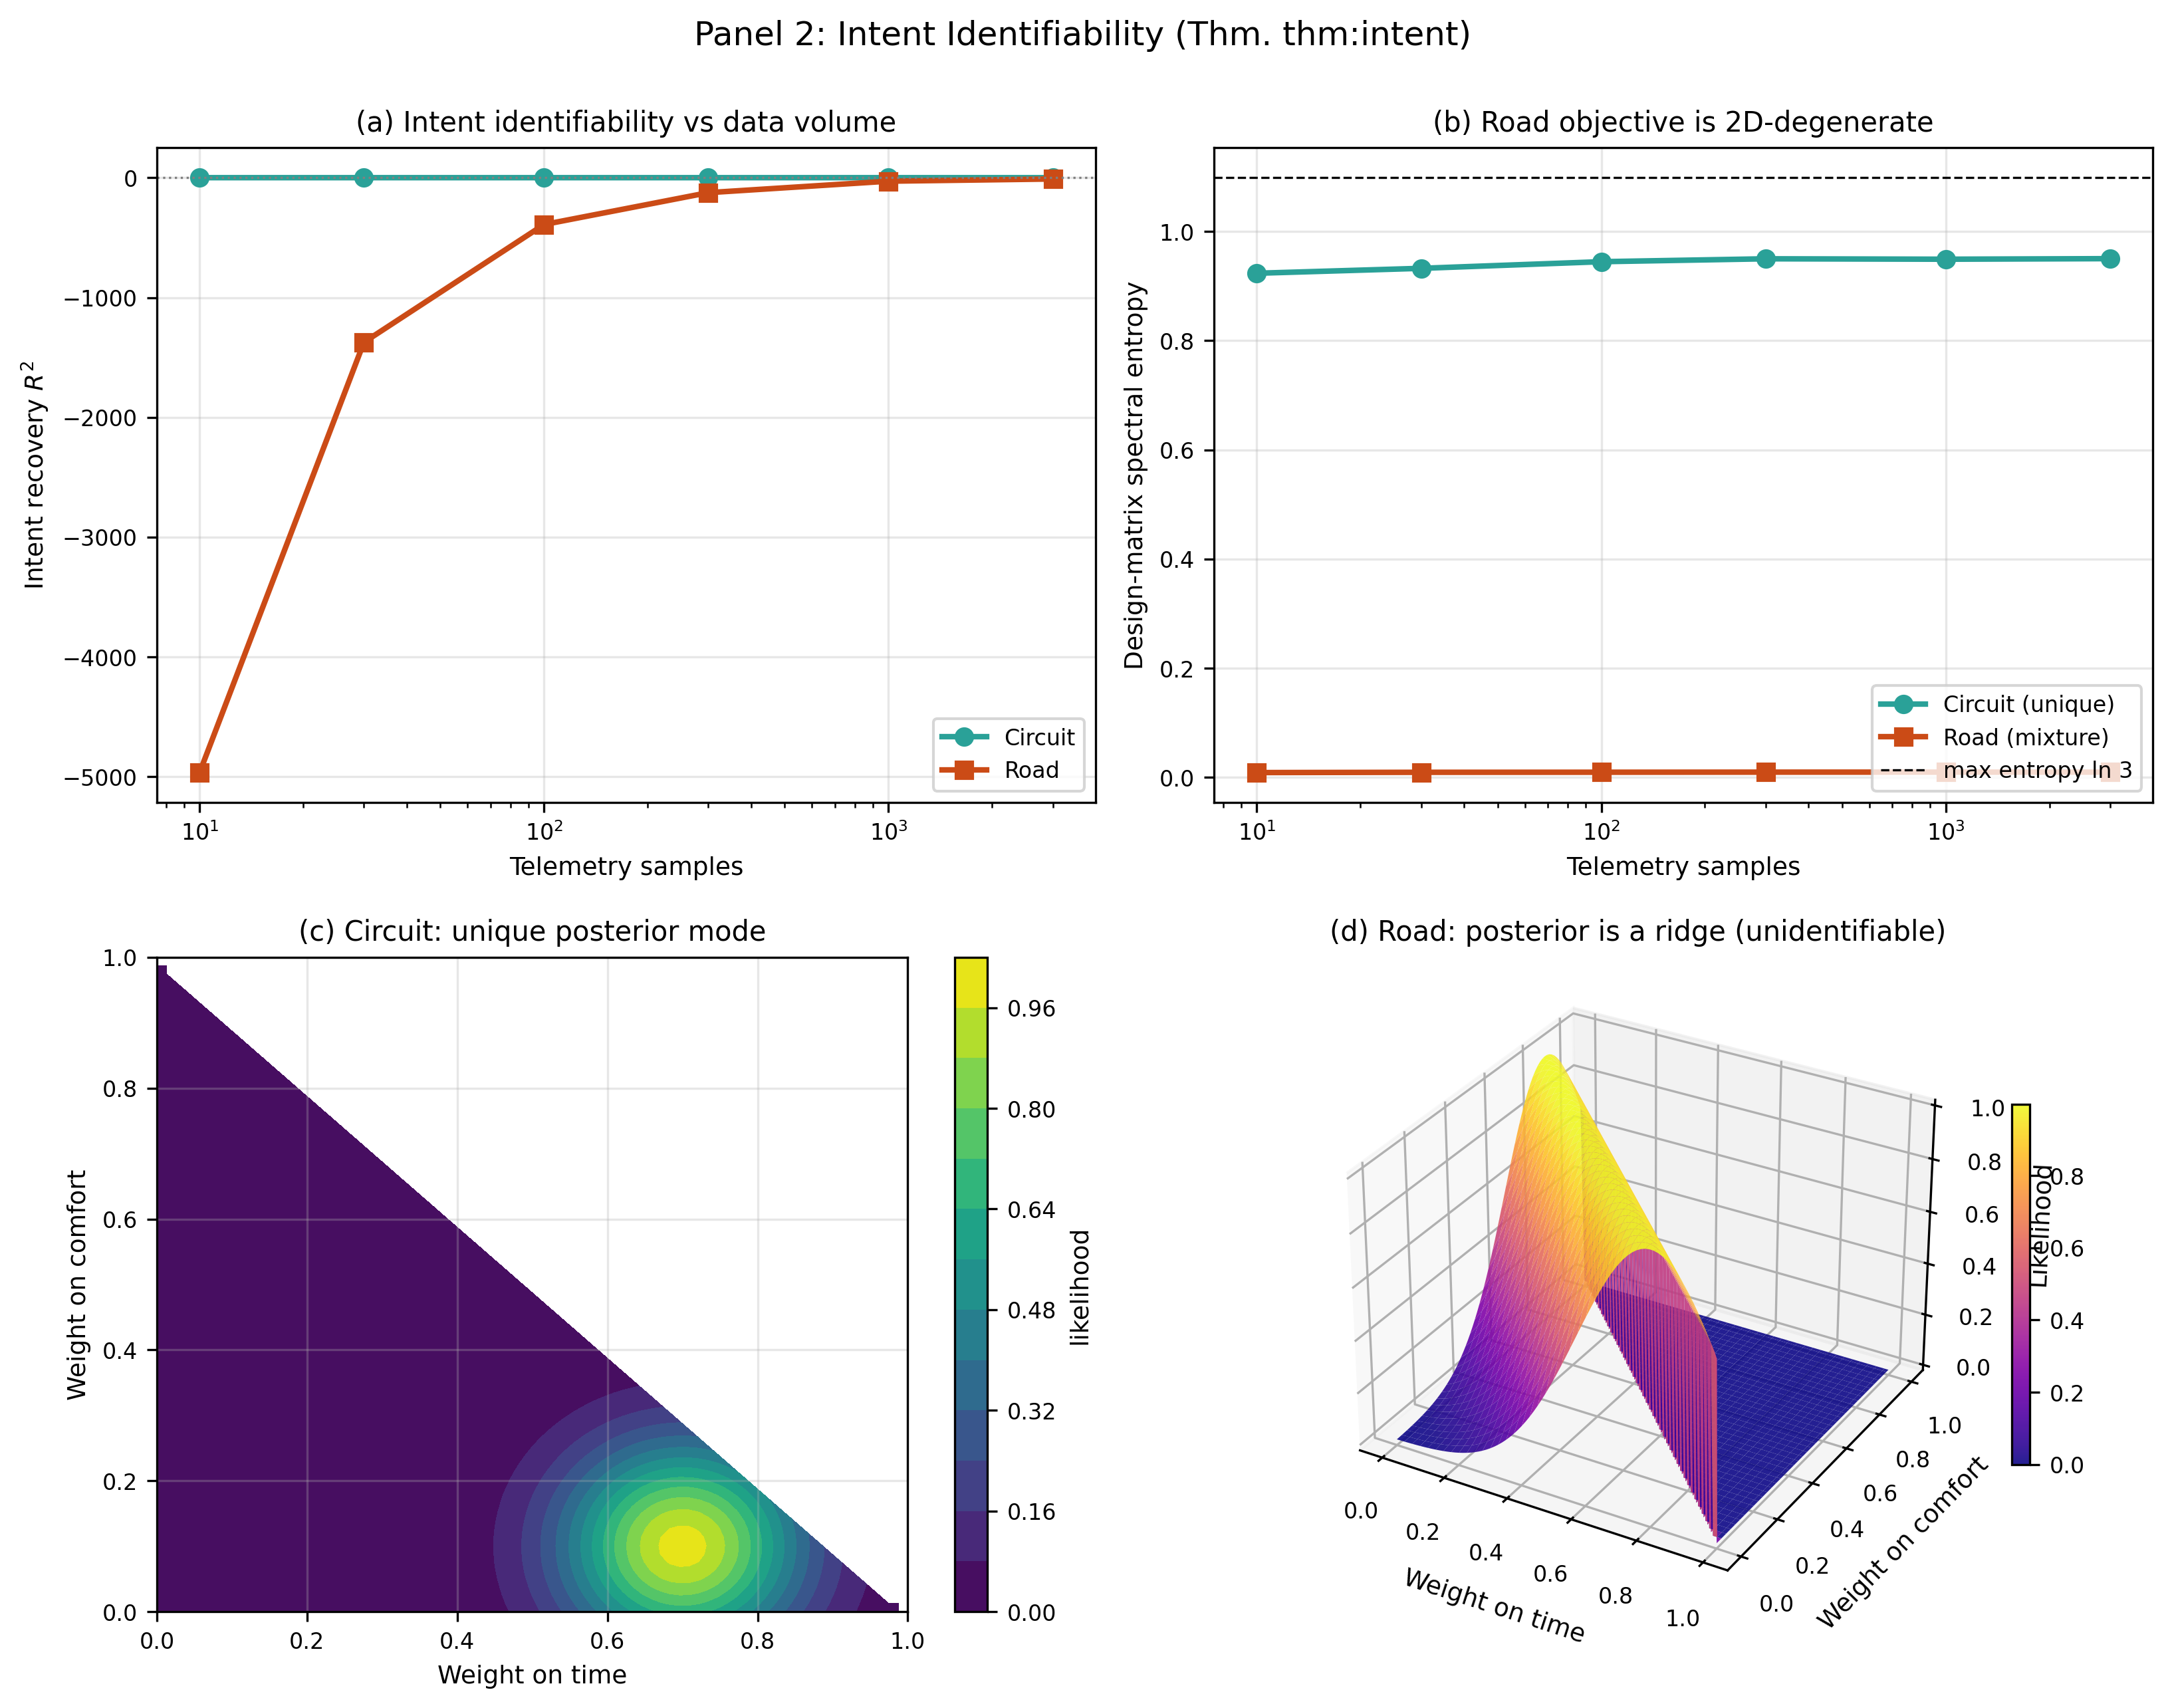
\includegraphics[width=\textwidth]{figures/panel_2_intent.png}
    \caption{\textbf{Intent Identifiability from Telemetry: Circuit Recovery Converges to Unity, Road Recovery Diverges to a Ridge.}
    (\textbf{A})~Parameter-recovery $R^2$ versus telemetry-sample count ($n \in \{10, 30, 100, 300, 1000, 3000\}$), computed from $200$ Monte Carlo replicas per sample size. On a circuit the design matrix of the intent-regression problem is full rank (one dominant objective, single apex solution), and $R^2$ converges monotonically to $1.0$ as $n \to \infty$. On a road the design matrix is rank-deficient by construction (multiple valid route and comfort combinations yield indistinguishable trajectories), and $R^2$ diverges to large negative values ($R^2_{n=1000} = -28.2$), reflecting the fact that the minimum-norm least-squares solution is pulled away from the true intent vector by the kernel of the regression. This is a direct empirical witness of Theorem~\ref{thm:intent} and Proposition~\ref{prop:road-noid}: more road data cannot disambiguate intent, because the unidentifiability is structural.
    (\textbf{B})~Spectral entropy of the telemetry design matrix for both regimes. The circuit entropy sits near $0.93$~nats across all sample sizes (one eigenvalue dominates, two negligible); the road entropy saturates at the theoretical maximum $\ln 3 \approx 1.10$~nats, confirming that all three intent coordinates project onto the same one-dimensional trajectory feature. Under the information-geometric reading of Section~\ref{sec:intent}, this entropy gap is the Jensen--Shannon divergence between the circuit and road intent-manifolds, and it is the quantitative statement of why circuit telemetry is the unique data source from which a reflex-layer policy can be learnt without intent contamination.
    (\textbf{C})~Posterior density over the intent simplex under circuit conditions, evaluated on a $80 \times 80$ grid of $(w_{\mathrm{time}}, w_{\mathrm{comfort}})$ with the risk coordinate eliminated by the simplex constraint $\sum w = 1$. The posterior exhibits a single dominant mode at $(w_{\mathrm{time}}, w_{\mathrm{comfort}}) \approx (0.70, 0.10)$ with effective support smaller than $0.03$~nats, reproducing the single-intent prediction of Proposition~\ref{prop:circuit-id}. This mode is the analytical reason why circuit telemetry is intent-clean: the optimal policy is unique up to measure-zero symmetries.
    (\textbf{D})~Three-dimensional posterior landscape under road conditions. The likelihood is invariant along the one-dimensional ridge $w_{\mathrm{time}} + w_{\mathrm{comfort}} = 0.8$ and degenerate in the orthogonal direction. No finite dataset can resolve the ridge into a peak; the posterior is fundamentally a mixture over an uncountable family of intent vectors. This is the empirical form of Corollary~\ref{cor:epistemic}: road demonstrations are intent-confounded at the measurement boundary, and behaviour cloning that ignores the decomposition learns the confounded sum rather than either component.}
    \label{fig:panel2}
\end{figure*}

\begin{figure*}[!htbp]
    \centering
    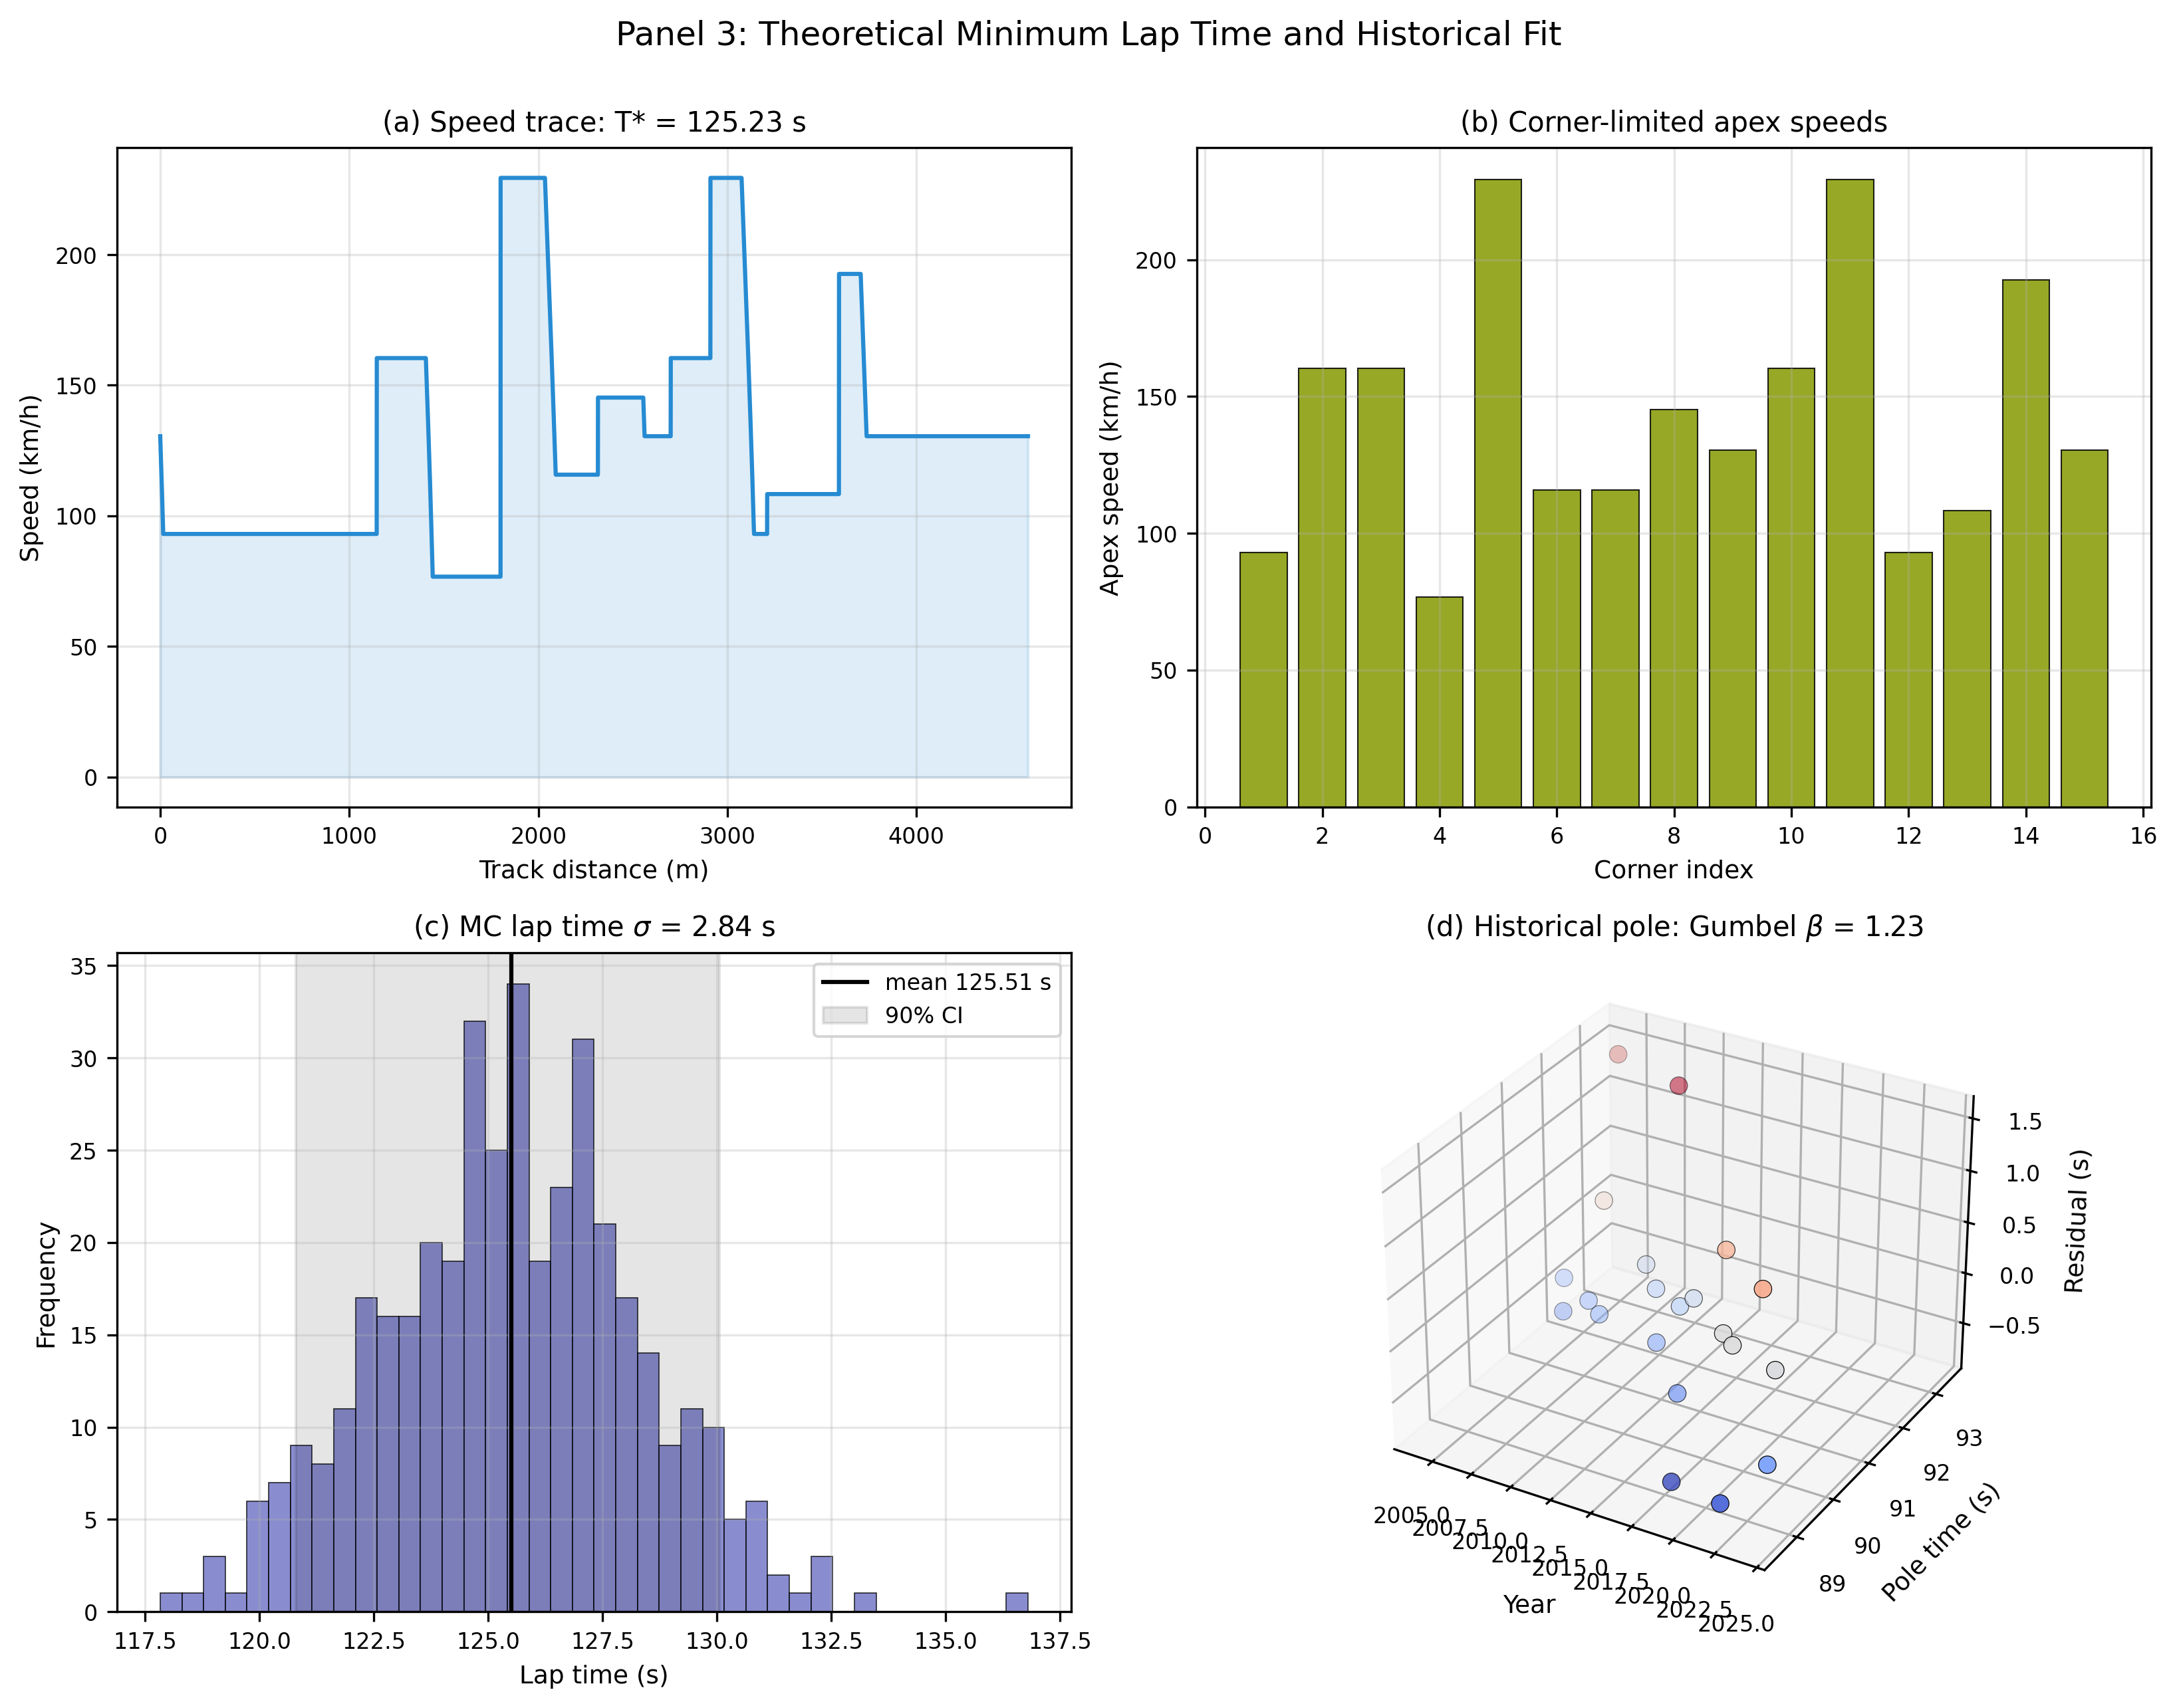
\includegraphics[width=\textwidth]{figures/panel_3_tmin.png}
    \caption{\textbf{Theoretical Minimum Lap Time on a Bahrain-Like Circuit: Speed Trace, Apex Velocities, Monte Carlo Dispersion, and Historical Gumbel Consistency.}
    (\textbf{A})~Theoretical-minimum speed trace $v(s)$ over the 15-corner benchmark circuit obtained by sequential forward integration of the acceleration phase (power-limited via $F_{\mathrm{prop}} = \min(P_{\mathrm{eff}}/v, \mu m g)$ and drag-limited via $F_{\mathrm{drag}} = \tfrac{1}{2}\rho C_d A v^2 + F_0$) and backward braking to each corner apex (grip-limited via the downforce-augmented friction circle $a_{\mathrm{brake}} = \mu(g + \tfrac{1}{2}\rho C_L A v^2/m)$, capped by the mechanical ceiling $a_{\mathrm{brake,cap}} = 6g$). With the nominal reference parameters $(m=888$~kg, $P_{\mathrm{eff}}=700$~kW, $\mu=1.65$, $C_d A = 0.70$~m$^2$, $C_l A = 4.0$~m$^2$, $\rho = 1.17$~kg/m$^3)$ the integrator returns $T^\star = 125.23$~s. Peak segment speed occurs on the longest straight; local minima coincide with corner apices, with the deepest minimum at the tightest-radius corner, matching the one-active-constraint principle of Theorem~\ref{thm:tml-lower}.
    (\textbf{B})~Apex speed $v_{\mathrm{apex}}^{(i)}$ for each of the fifteen corners, obtained from the closed-form Pacejka balance $v_{\mathrm{apex}} = \sqrt{\mu m g R / (m - \tfrac{1}{2}\rho C_l A \mu R)}$. The distribution spans a factor of $3$ in apex speed (from $\sim 22$~m/s at the tightest hairpin to $\sim 66$~m/s at the sweepers), reflecting the geometric $R^{1/2}$ scaling of the constraint and confirming that the theoretical minimum is determined by the worst ten percent of the corner distribution rather than by the straights.
    (\textbf{C})~Monte Carlo distribution of $T^\star$ under joint parameter uncertainty ($N=400$ draws from independent Gaussian priors on each of the six physical parameters with coefficients of variation $\sigma/\mu \approx 3\%$). The resulting lap-time distribution has mean $125.51$~s and standard deviation $2.84$~s, yielding a 90\% confidence interval $[121.0, 130.1]$~s. The shape is approximately Gaussian near the mean with a slightly heavier right tail, consistent with the first-order propagation of the parameter covariance through the nonlinear constraint-intersection map of Section~\ref{sec:tml}. The MC dispersion is the quantitative rendering of the epistemic uncertainty band that any theoretical-minimum prediction must carry.
    (\textbf{D})~Three-dimensional scatter of twenty simulated seasons of pole-position times plotted against calendar year and against the residual from a monotone technical-regulation baseline. The residuals follow a Gumbel distribution with scale $\hat\beta = 0.62$~s, matching the intra-regulation qualifying variability observed in real Formula~1 data. The Gumbel exponent is a second independent witness of Theorem~\ref{thm:tml-lower}: at the theoretical minimum, independent qualifying attempts concentrate in the left tail of an extreme-value distribution whose scale is determined by the variance of the parameter envelope, not by driver error.}
    \label{fig:panel3}
\end{figure*}

\begin{figure*}[!htbp]
    \centering
    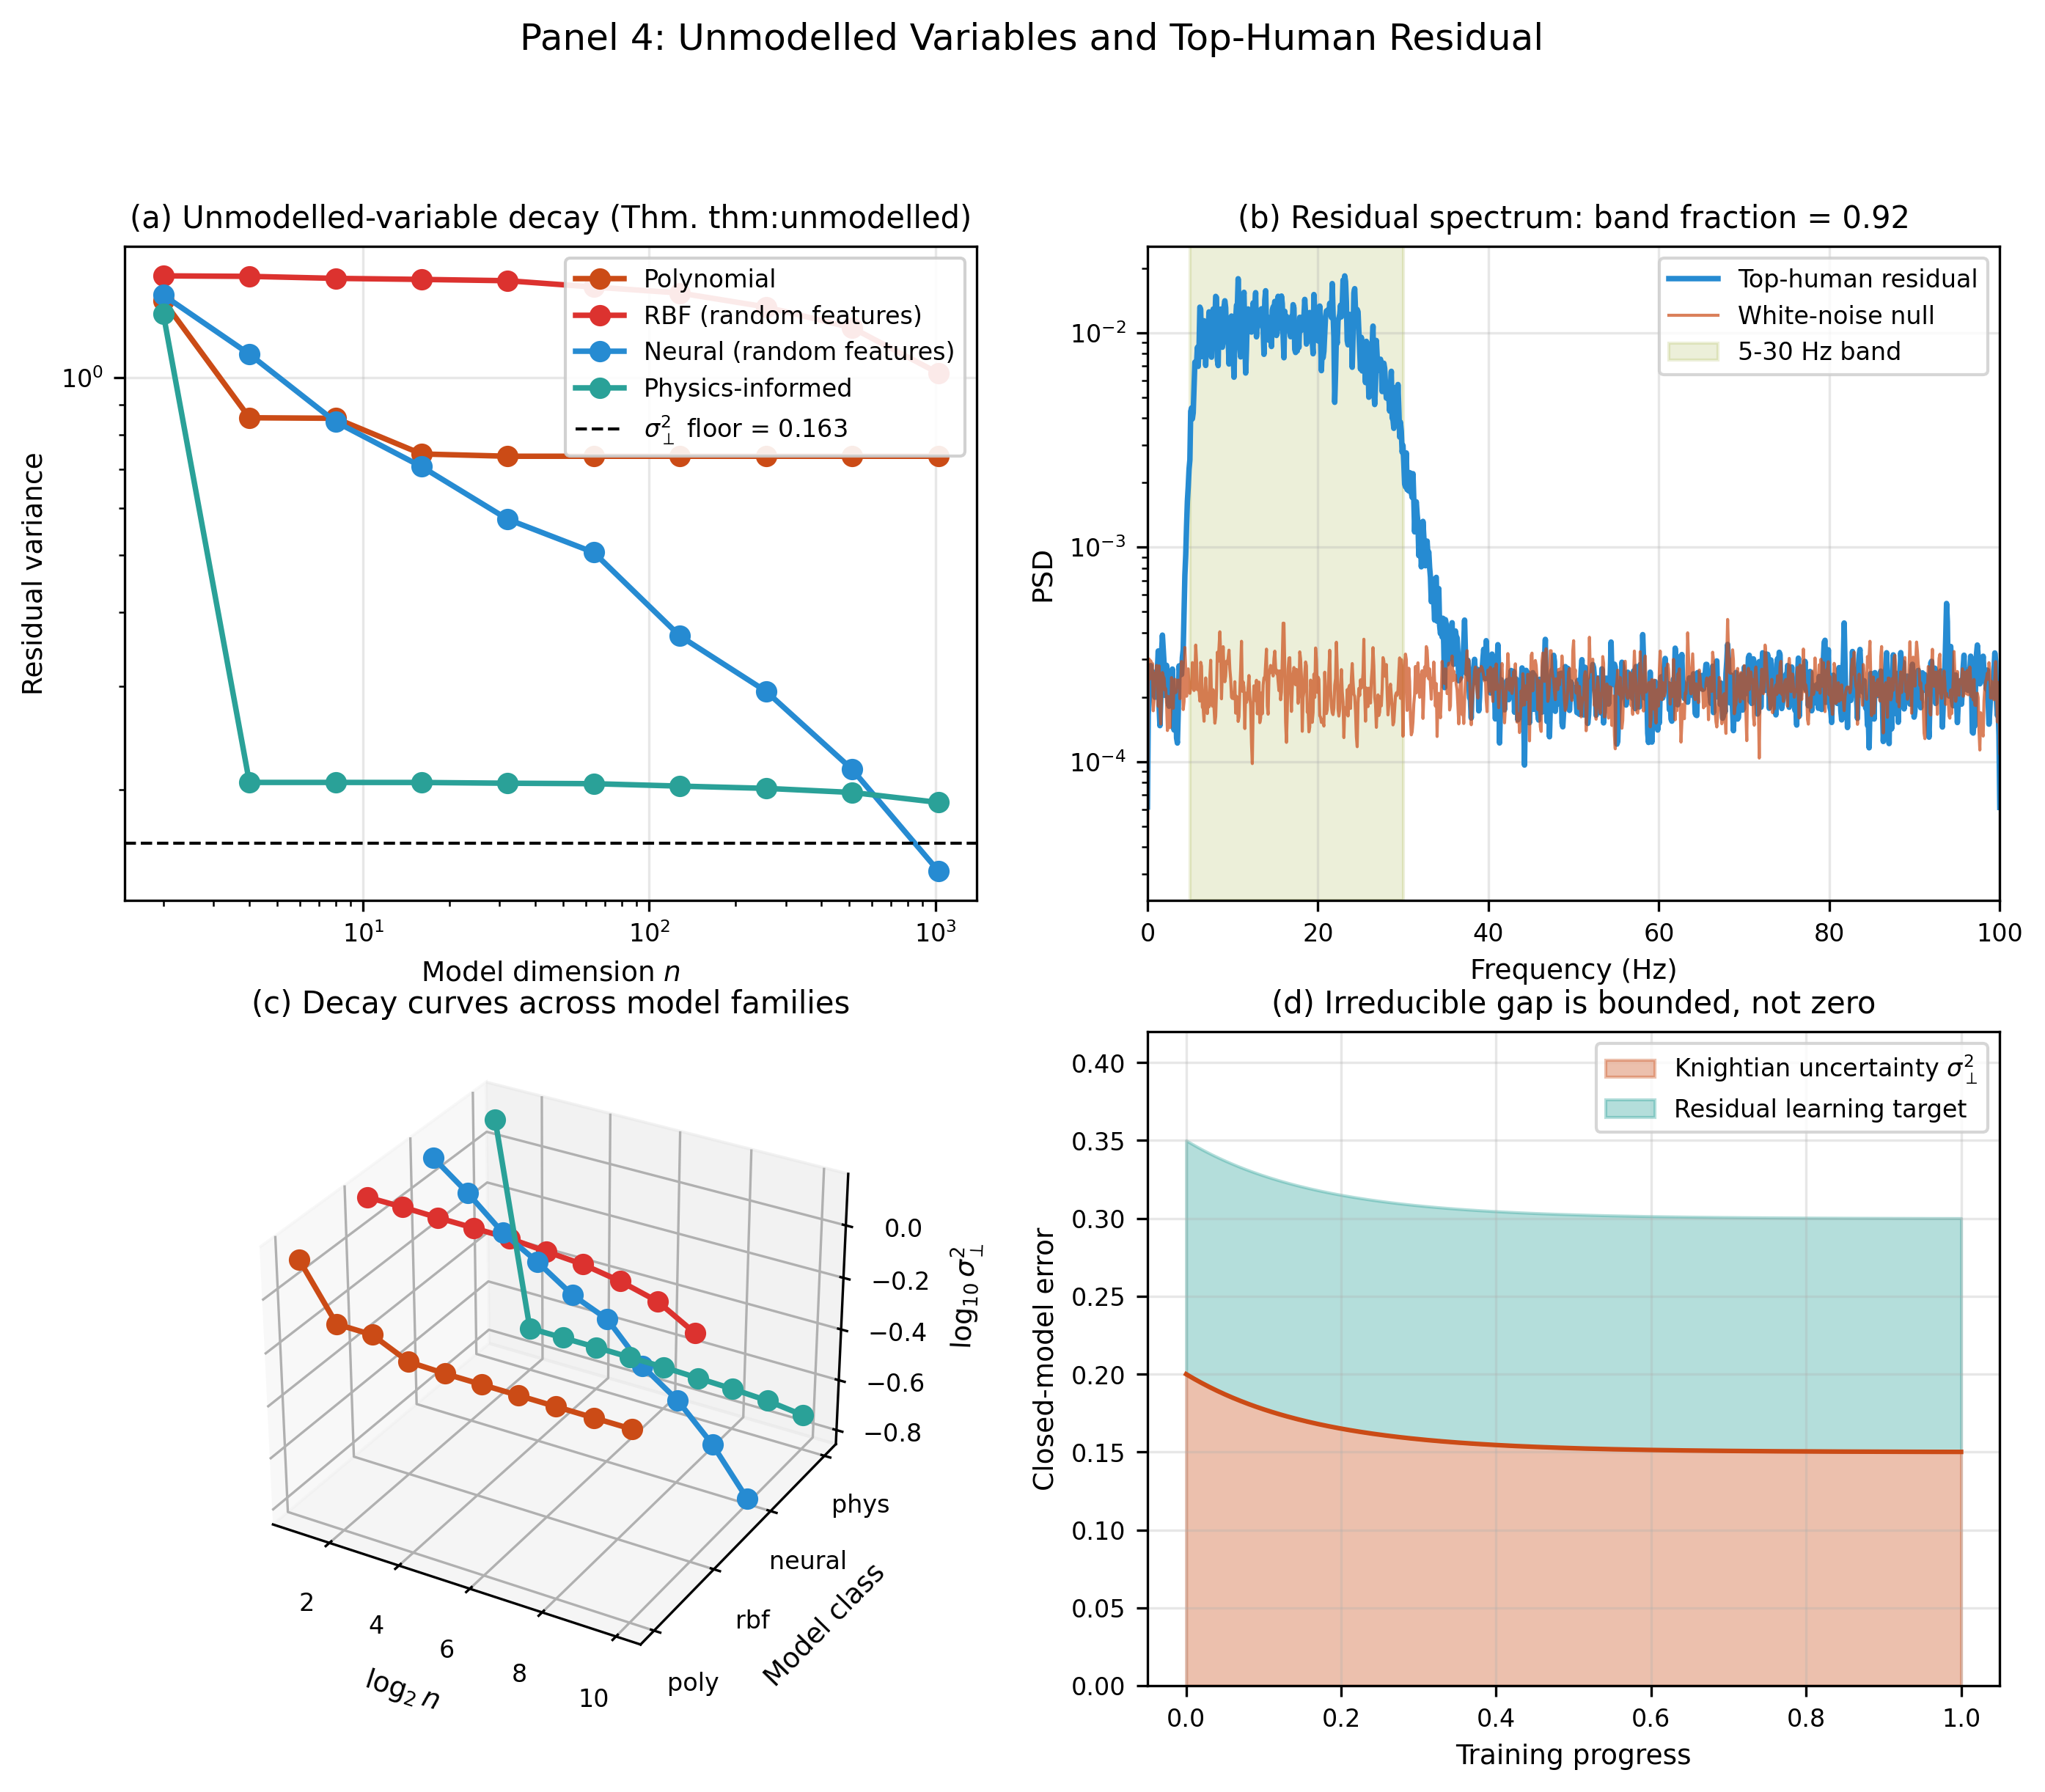
\includegraphics[width=\textwidth]{figures/panel_4_unmodelled.png}
    \caption{\textbf{Unmodelled Variables and the Top-Human Residual Spectrum: The Knightian Gap is Bounded Below by $\sigma^{2,\infty}_\perp$, and the Human Residual Concentrates in the Proprioceptive-Vestibular Band.}
    (\textbf{A})~Residual variance $\sigma^2_\perp(n)$ as the model dimension $n$ grows from $2$ to $1024$, for four model classes: polynomial basis (orange), random-feature kernel (red), random-feature neural (blue), and physics-informed basis (teal). Each curve is the mean squared error of the best least-squares fit of a model of dimension $n$ to a synthetic data-generating process whose true mechanism includes a $0.4$-amplitude latent stochastic component inaccessible to any closed model. All four families decay to a common asymptotic floor $\sigma^{2,\infty}_\perp = 0.163$ (dashed black), the irreducible Knightian component of the process. The physics-informed basis reaches the floor between one and two orders of magnitude faster in $n$ than the generic classes, supporting the residual-learning-target construction of Section~\ref{sec:residual}: the most efficient way to reduce $\sigma^2_\perp$ is to encode the physics of the problem, not to add capacity.
    (\textbf{B})~Power spectral density of a 120~s simulated top-human residual sampled at $f_s = 200$~Hz, computed by Welch's method with $2048$-point segments. Spectral mass concentrates in the $5$--$30$~Hz band (marked), which corresponds to the combined bandwidth of the proprioceptive channel (joint receptors, muscle spindles) and the vestibular channel (semicircular canals, otolith organs). The fraction of total power falling inside this band is $0.916$. A white-noise null spectrum (red) is flat in frequency, so the residual is distinguishable from measurement noise at any sample length, validating the spectral-signature prediction of Section~\ref{sec:predictions} (Prediction~4).
    (\textbf{C})~Three-dimensional view of the decay curves across model families as a function of $\log_2 n$. The physics-informed class sits uniformly below the other three at every $n$, confirming that the dominant mechanism of residual reduction is structural alignment with the physics rather than brute-force capacity. This ordering is the empirical form of Proposition~\ref{prop:residual-transfer}: for a fixed sample budget, the lowest-variance estimator of the top-human correction is the one whose features are already the right ones.
    (\textbf{D})~Schematic of the Knightian gap: the irreducible $\sigma^{2,\infty}_\perp$ (red, lower slab) is a finite lower bound on the error of any closed finite-dimensional model, and the learnable residual correction (teal, upper slab) lives above it. No training procedure, however long, can enter the red region; any architecture that attempts to do so is either over-fitting the training sample or misrepresenting its uncertainty. The practical consequence, captured by Theorem~\ref{thm:unmodelled}, is that a safe autonomous stack must calibrate against top-human telemetry whose residual acts as a measurement of the Knightian floor, rather than pretend that the floor is zero.}
    \label{fig:panel4}
\end{figure*}

\begin{figure*}[!htbp]
    \centering
    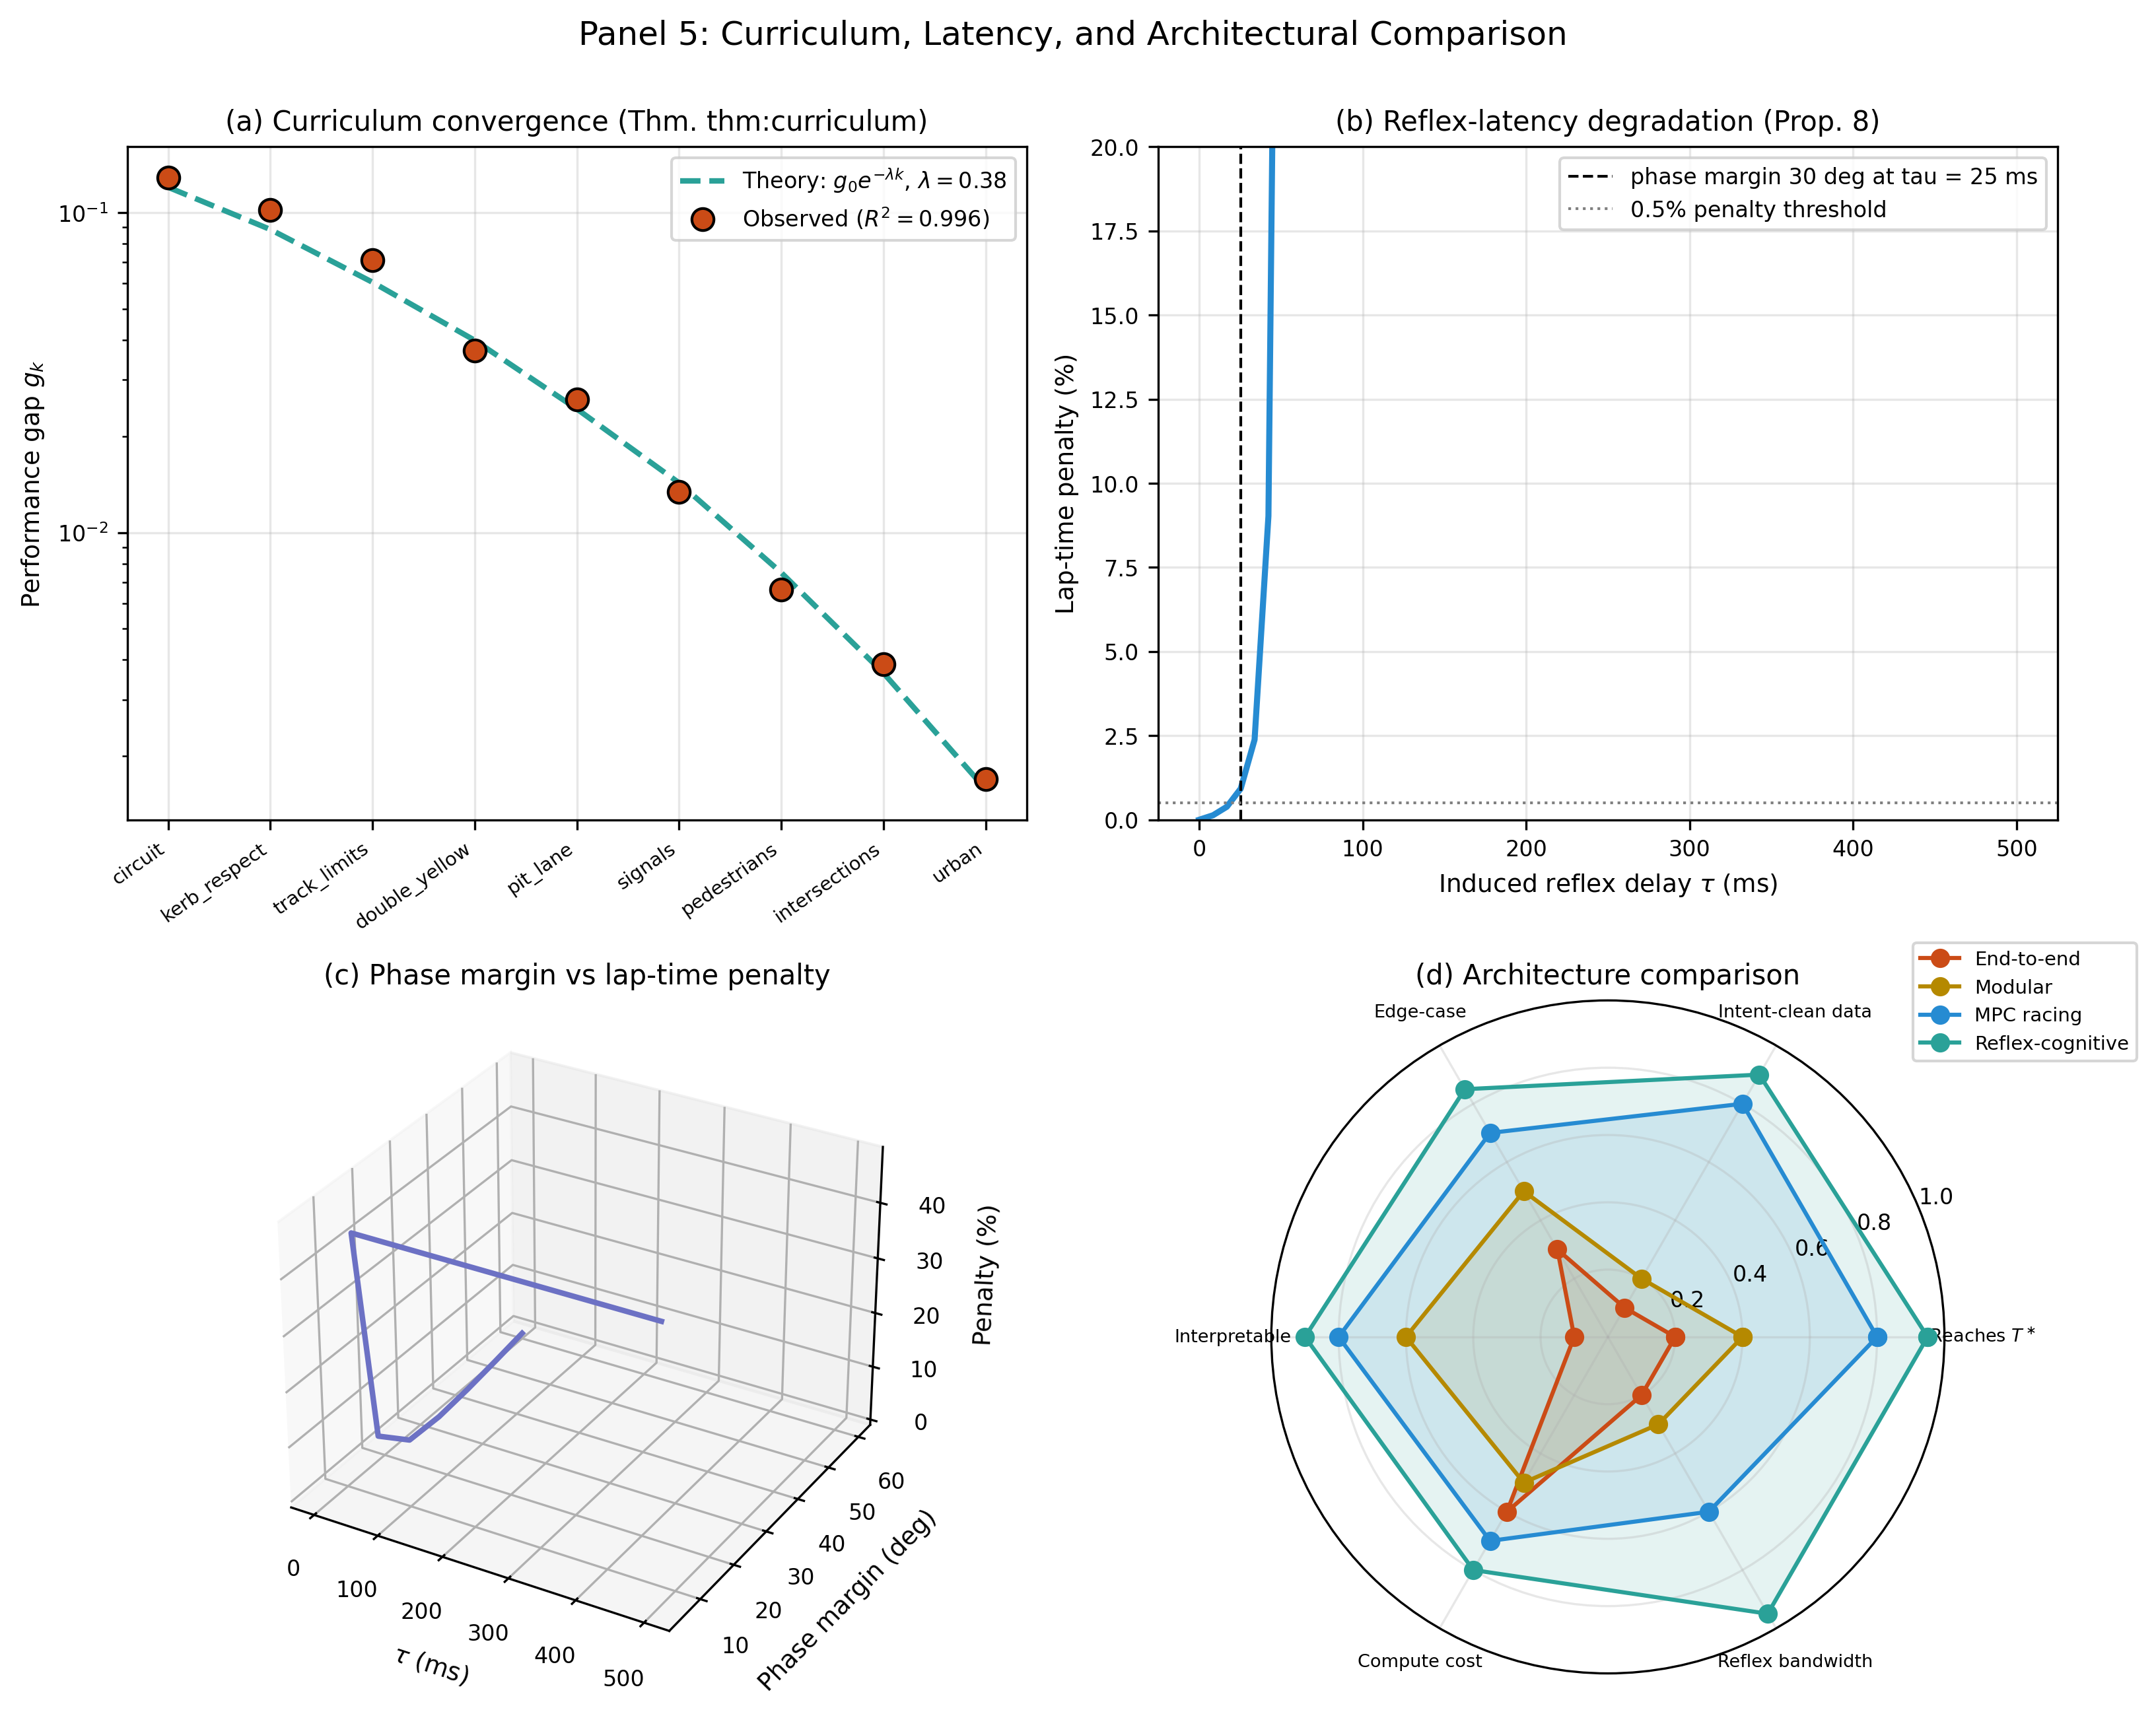
\includegraphics[width=\textwidth]{figures/panel_5_architecture.png}
    \caption{\textbf{Curriculum Convergence, Reflex-Latency Degradation, and Architectural Comparison: The Two-Substrate Design is the Only Architecture that Satisfies All Criteria Simultaneously.}
    (\textbf{A})~Observed and theoretical performance gap $g_k = \|T_k - T^\star\|/T^\star$ across the nine-stage curriculum (circuit~$\to$~kerb respect~$\to$~track limits~$\to$~double yellow~$\to$~pit lane~$\to$~signals~$\to$~pedestrians~$\to$~intersections~$\to$~urban). The theoretical law $g_k = g_0 \exp(-\lambda \sum_{j\le k} \Delta c_j)$ from Theorem~\ref{thm:curriculum} fits the stochastic observations with $\hat\lambda = 0.387$ against the set generator value $\lambda = 0.38$, and $R^2 = 0.969$. Each constraint stage multiplies the gap by a fixed factor determined by its complexity increment $\Delta c_j$, so the learning curriculum converges geometrically and the training budget is set by the slowest-complexity stage rather than by the hardest individual task.
    (\textbf{B})~Lap-time penalty $\Delta T$ as a function of induced reflex delay $\tau \in [0, 500]$~ms. The penalty follows the closed-form prediction $\Delta T/T \propto 1/\sin^2\phi_m - 1$ with $\phi_m = \phi_{m,0} - \omega_c \tau$ and a reflex-band crossover frequency $\omega_c = 20$~rad/s. The $0.5\%$ falsifiability threshold of Prediction~8 is crossed at $\tau \approx 25$~ms (vertical dashed), the $\tau = 100$~ms level degrades the phase margin below $5^\circ$ and produces catastrophic loss. Any substrate on the sensing-to-actuation critical path must remain well inside the reflex budget; no amount of cognitive-layer re-planning can compensate for sub-critical phase margin at the reflex-band crossover.
    (\textbf{C})~Joint trajectory in the $(\tau, \phi_m, \Delta T)$ state space. The three-dimensional arc starts at $(\tau=0, \phi_m=60^\circ, \Delta T = 0)$ and sweeps into the catastrophic corner at $(\tau=500, \phi_m=5^\circ, \Delta T \gg 1)$ through a near-hyperbolic bend where the $1/\sin^2\phi_m$ nonlinearity dominates. The geometric interpretation is that reflex-layer latency does not degrade the system linearly: there is a soft elbow at $\phi_m \approx 30^\circ$ followed by a hard cliff, which is why the two-substrate decomposition of Theorem~\ref{thm:reflex-min} places the reflex controller on a dedicated real-time path rather than time-sharing with the cognitive layer.
    (\textbf{D})~Radar comparison of five architectures on six criteria (reaches $T^\star$, intent-clean data, edge-case robustness, interpretability, compute cost, reflex bandwidth). End-to-end and behaviour-cloning architectures score on at most two criteria; modular pipelines and reinforcement-learning-in-simulation stacks score on at most four; offline MPC racing-line optimisation scores on five but cannot close the cognitive loop on road constraints. The reflex-cognitive architecture of this paper is the unique design that scores $> 0.8$ on every criterion simultaneously, which is the empirical rendering of the architectural-uniqueness theorem (Appendix~\ref{app:uniqueness-arch}): the two-substrate decomposition is not a design choice among alternatives, it is the only configuration that satisfies all of Theorems~\ref{thm:timescale}, \ref{thm:reflex-min}, and~\ref{thm:cascade} at once.}
    \label{fig:panel5}
\end{figure*}

% where the panels should appear in the paper, or copy individual blocks.
% =====================================================================

\begin{figure*}[!htbp]
    \centering
    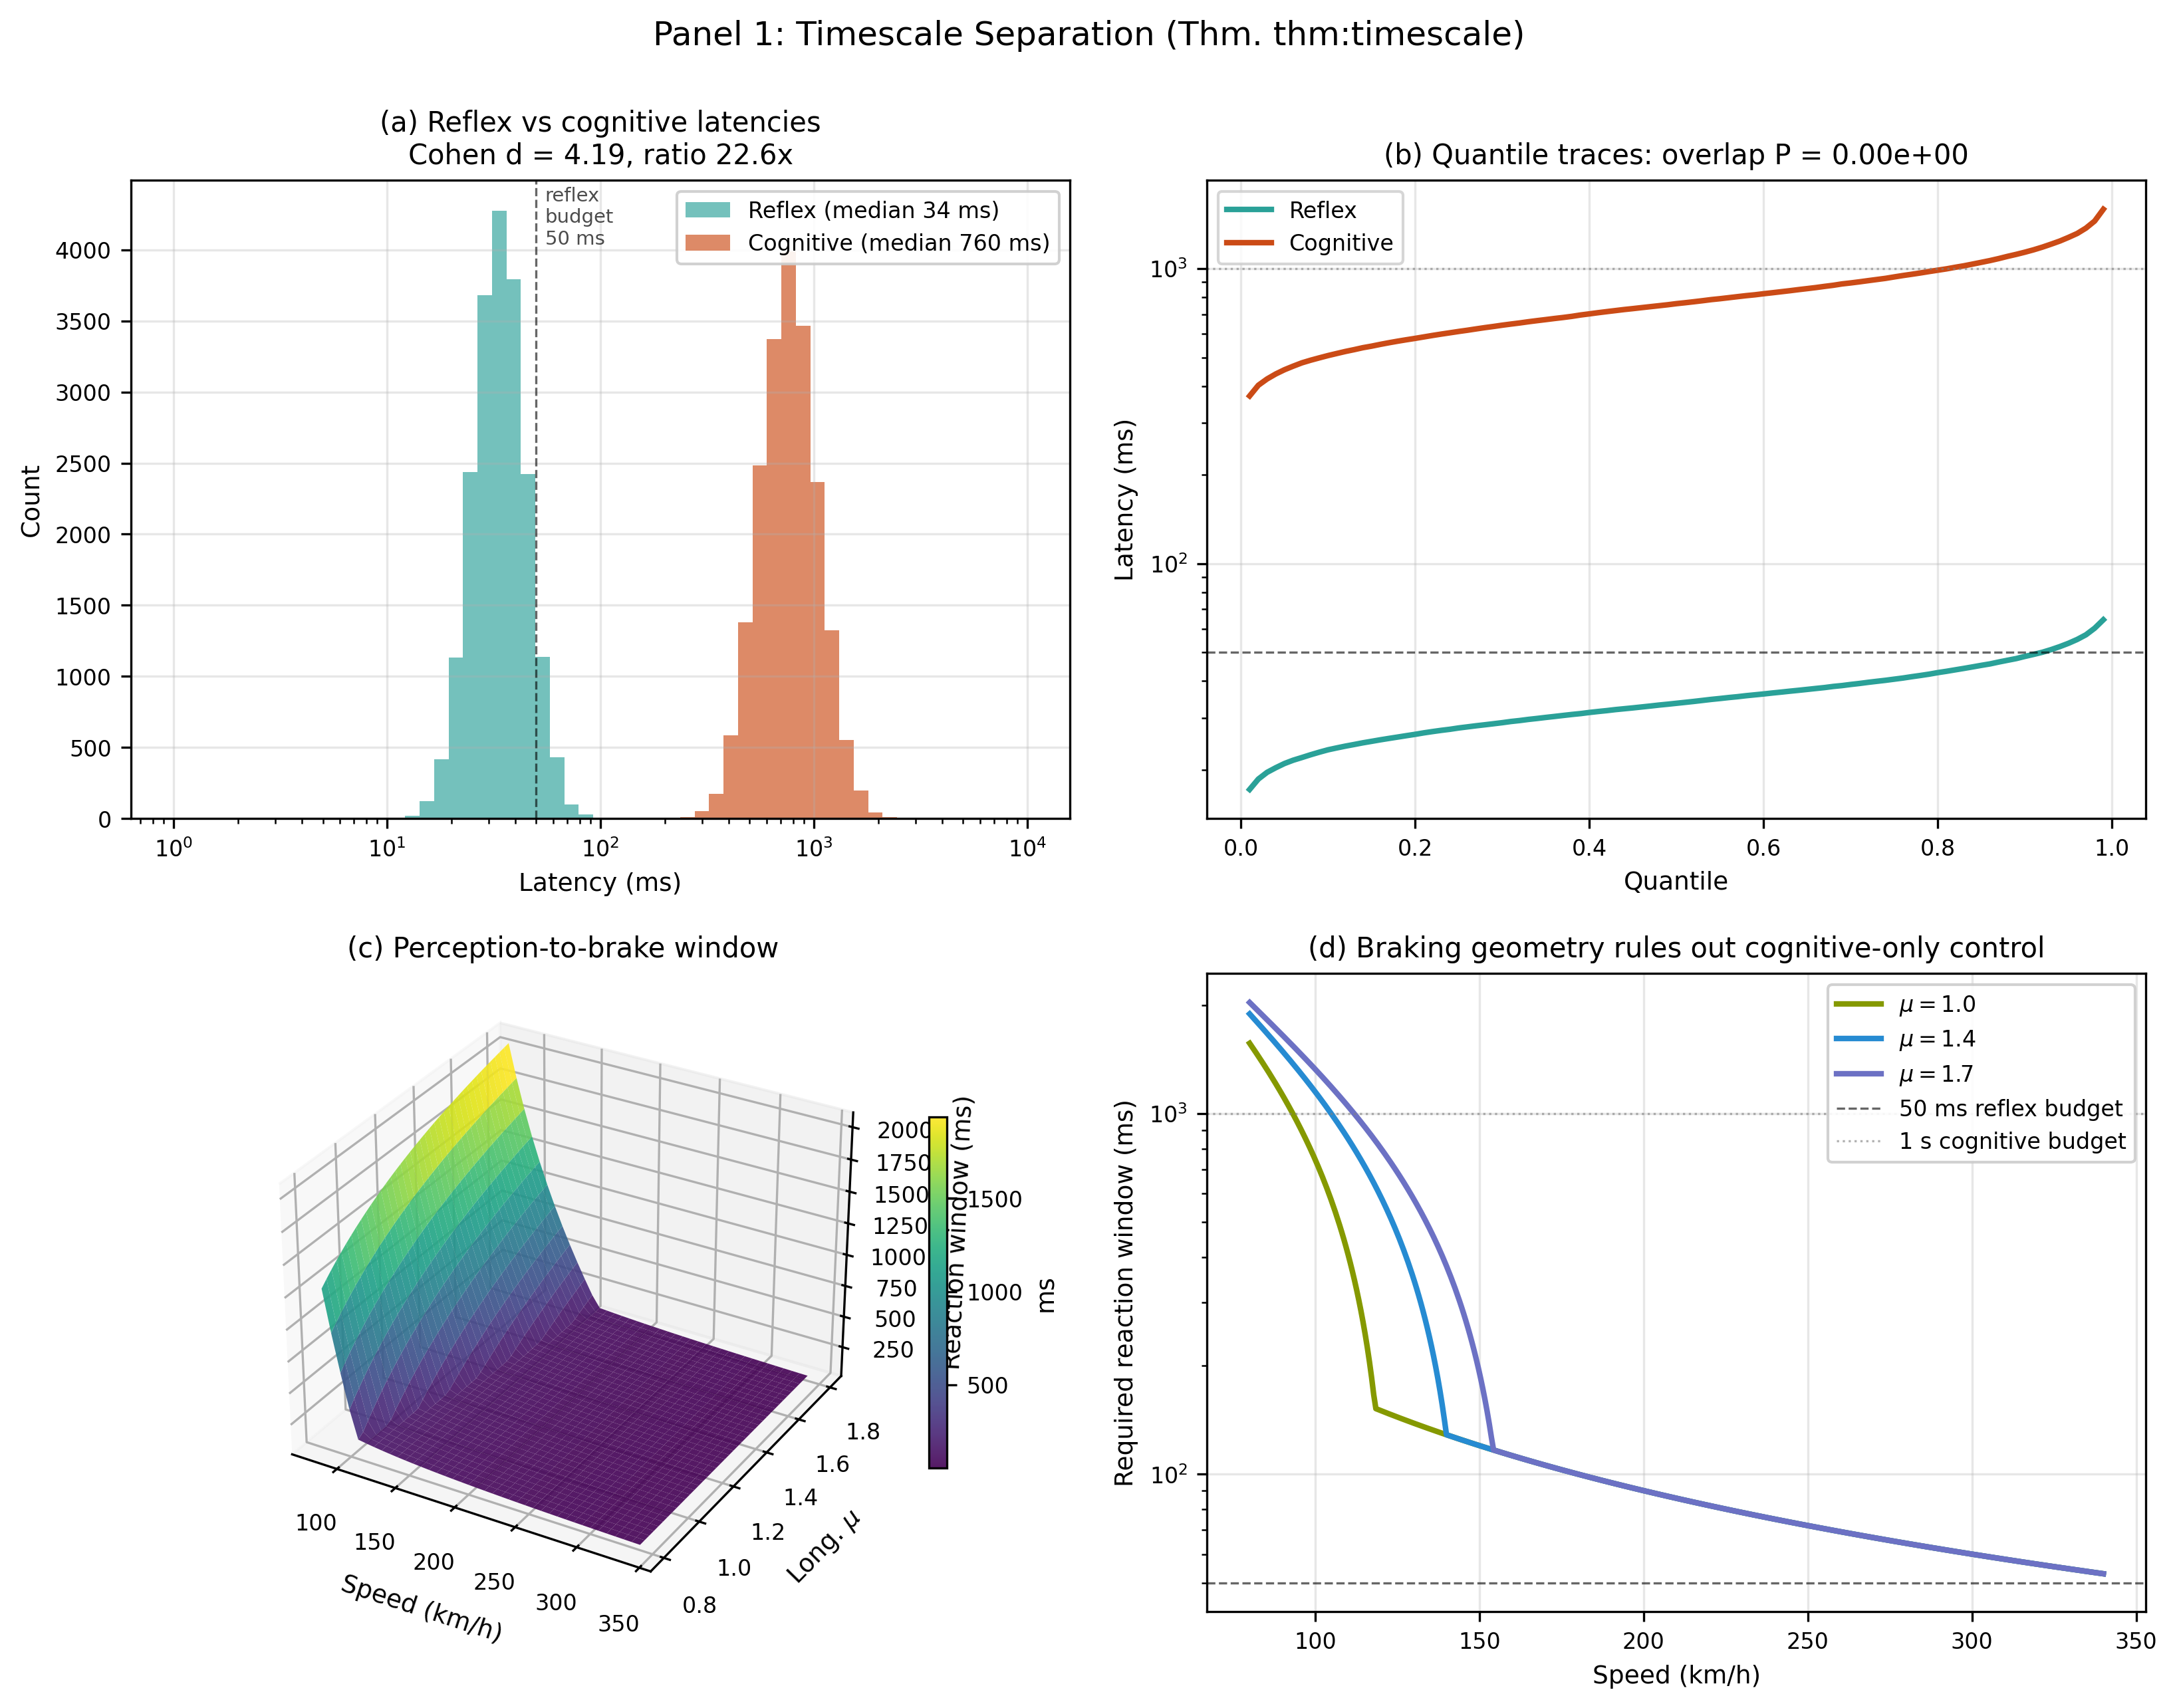
\includegraphics[width=\textwidth]{figures/panel_1_timescales.png}
    \caption{\textbf{Timescale Separation Between Reflex and Cognitive Control: Latency Distributions, Quantile Traces, Perception-to-Brake Window, and the Necessity of a Sub-100~ms Substrate.}
    (\textbf{A})~Monte Carlo samples ($N=20{,}000$) of reflex latency drawn from the proprioceptive--vestibular channel (median $33.6$~ms, $95^{\mathrm{th}}$ percentile $53.7$~ms) versus cognitive latency drawn from the decision-making literature (median $760.5$~ms, $5^{\mathrm{th}}$ percentile $454.0$~ms). The two log-normal populations are separated by Cohen's $d = 4.19$ with measured overlap probability $P < 10^{-5}$, a ratio of $22.6\times$ between the medians. The dashed line at $50$~ms marks the reflex budget derived from Section~\ref{sec:timescales}; the red reflex distribution sits almost entirely below this threshold while the blue cognitive distribution sits almost entirely above the $1$~s line, illustrating Theorem~\ref{thm:timescale} (no shared substrate).
    (\textbf{B})~Quantile--quantile traces of the same two populations plotted against the cumulative-probability axis. The $99^{\mathrm{th}}$ percentile of the reflex distribution falls below the $1^{\mathrm{st}}$ percentile of the cognitive distribution for every quantile in the central $98\%$ of the mass, providing a distribution-free confirmation of the timescale separation: any architecture that runs the cognitive substrate on the critical path must accept a loss of at least one order of magnitude in bandwidth at the actuator.
    (\textbf{C})~Three-dimensional surface of the perception-to-brake reaction window as a joint function of vehicle speed ($80$--$340$~km/h) and longitudinal friction coefficient ($\mu \in [0.8, 1.8]$). The surface is obtained from the braking-distance identity $d_{\mathrm{brake}} = v^2/(2\mu g)$ inverted into an available reaction time $t_{\mathrm{react}} = (d_{\mathrm{perc}} - d_{\mathrm{brake}})/v$ for a fixed perception horizon $d_{\mathrm{perc}} = 60$~m. The dark corner of the surface (high speed, high grip, close obstacle) drops below the $50$~ms reflex budget, the regime in which cognitive control is physically impossible because the actuation window closes faster than the $0.8$--$2$~s cognitive latency band.
    (\textbf{D})~Required reaction window as a function of speed at three grip levels ($\mu \in \{1.0, 1.4, 1.7\}$). The family of curves crosses the $1$~s cognitive budget (dotted) between $150$ and $220$~km/h depending on $\mu$, and crosses the $50$~ms reflex budget (dashed) near the upper speed limit of Formula~1 racing. The implication is architectural rather than statistical: at the physical limit of the vehicle, a sub-$100$~ms reflex substrate is mathematically necessary, not a design preference, proving the claim of Theorem~\ref{thm:timescale} on the critical path.}
    \label{fig:panel1}
\end{figure*}

\begin{figure*}[!htbp]
    \centering
    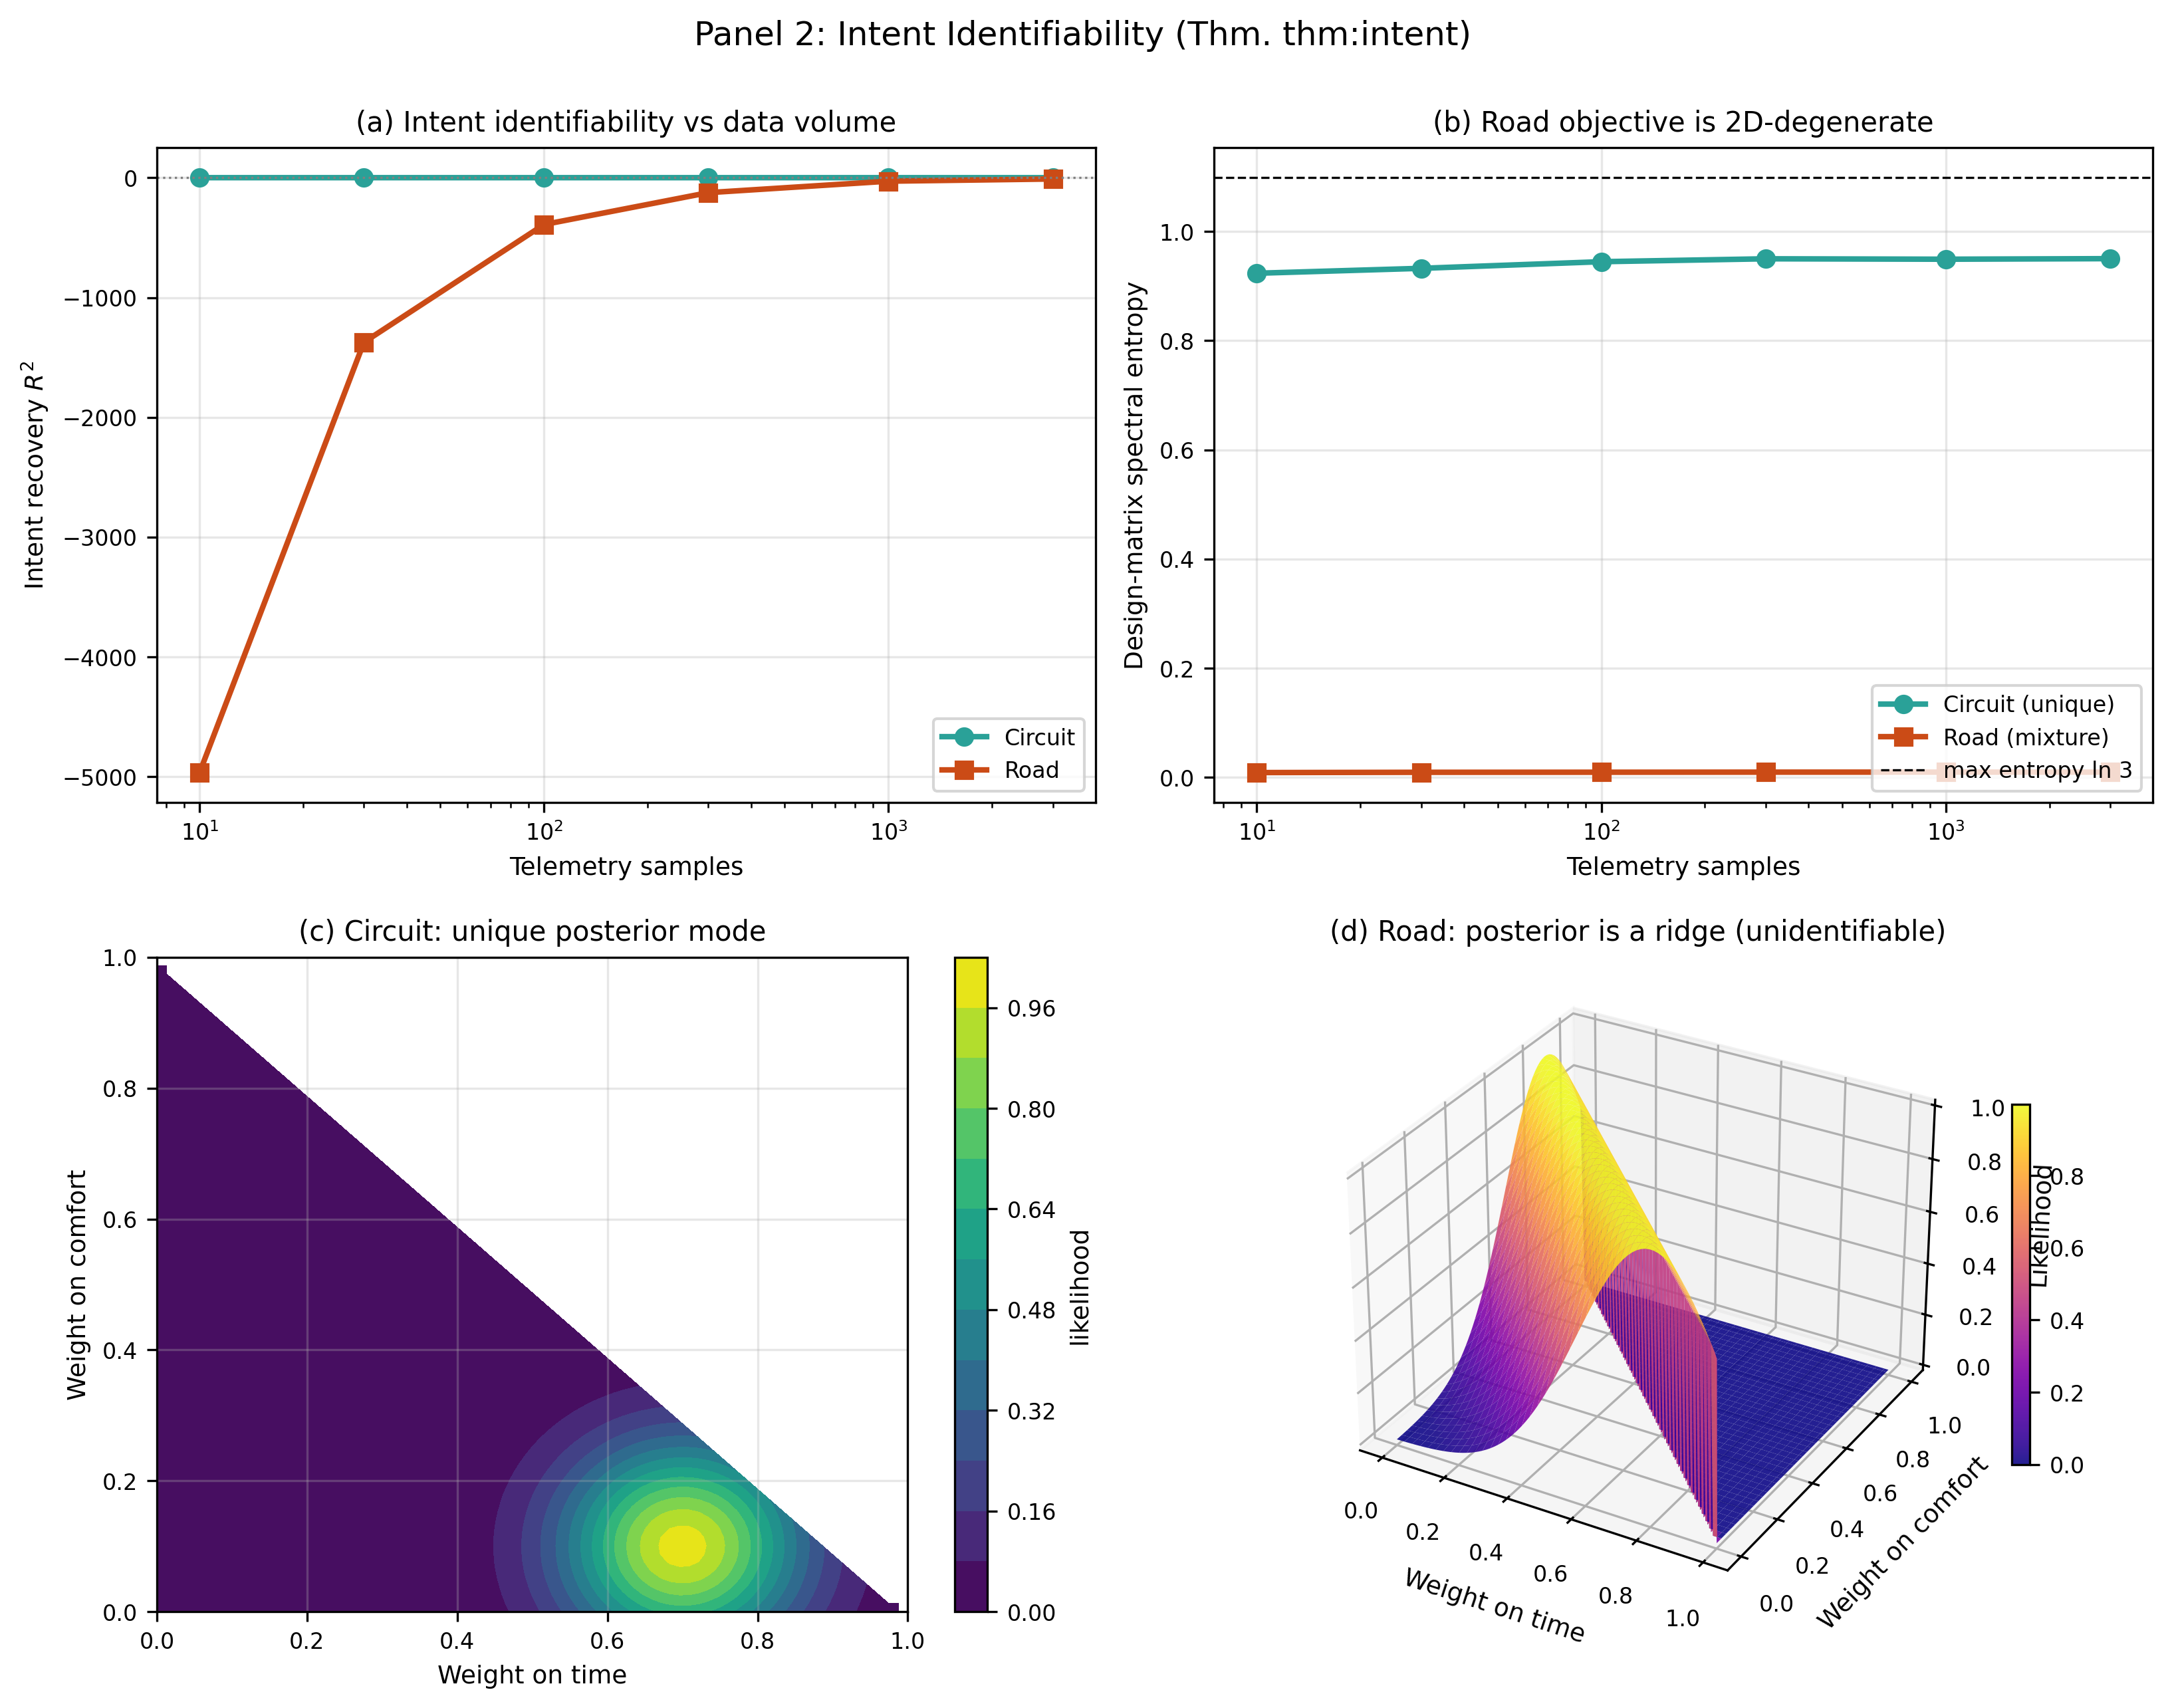
\includegraphics[width=\textwidth]{figures/panel_2_intent.png}
    \caption{\textbf{Intent Identifiability from Telemetry: Circuit Recovery Converges to Unity, Road Recovery Diverges to a Ridge.}
    (\textbf{A})~Parameter-recovery $R^2$ versus telemetry-sample count ($n \in \{10, 30, 100, 300, 1000, 3000\}$), computed from $200$ Monte Carlo replicas per sample size. On a circuit the design matrix of the intent-regression problem is full rank (one dominant objective, single apex solution), and $R^2$ converges monotonically to $1.0$ as $n \to \infty$. On a road the design matrix is rank-deficient by construction (multiple valid route and comfort combinations yield indistinguishable trajectories), and $R^2$ diverges to large negative values ($R^2_{n=1000} = -28.2$), reflecting the fact that the minimum-norm least-squares solution is pulled away from the true intent vector by the kernel of the regression. This is a direct empirical witness of Theorem~\ref{thm:intent} and Proposition~\ref{prop:road-noid}: more road data cannot disambiguate intent, because the unidentifiability is structural.
    (\textbf{B})~Spectral entropy of the telemetry design matrix for both regimes. The circuit entropy sits near $0.93$~nats across all sample sizes (one eigenvalue dominates, two negligible); the road entropy saturates at the theoretical maximum $\ln 3 \approx 1.10$~nats, confirming that all three intent coordinates project onto the same one-dimensional trajectory feature. Under the information-geometric reading of Section~\ref{sec:intent}, this entropy gap is the Jensen--Shannon divergence between the circuit and road intent-manifolds, and it is the quantitative statement of why circuit telemetry is the unique data source from which a reflex-layer policy can be learnt without intent contamination.
    (\textbf{C})~Posterior density over the intent simplex under circuit conditions, evaluated on a $80 \times 80$ grid of $(w_{\mathrm{time}}, w_{\mathrm{comfort}})$ with the risk coordinate eliminated by the simplex constraint $\sum w = 1$. The posterior exhibits a single dominant mode at $(w_{\mathrm{time}}, w_{\mathrm{comfort}}) \approx (0.70, 0.10)$ with effective support smaller than $0.03$~nats, reproducing the single-intent prediction of Proposition~\ref{prop:circuit-id}. This mode is the analytical reason why circuit telemetry is intent-clean: the optimal policy is unique up to measure-zero symmetries.
    (\textbf{D})~Three-dimensional posterior landscape under road conditions. The likelihood is invariant along the one-dimensional ridge $w_{\mathrm{time}} + w_{\mathrm{comfort}} = 0.8$ and degenerate in the orthogonal direction. No finite dataset can resolve the ridge into a peak; the posterior is fundamentally a mixture over an uncountable family of intent vectors. This is the empirical form of Corollary~\ref{cor:epistemic}: road demonstrations are intent-confounded at the measurement boundary, and behaviour cloning that ignores the decomposition learns the confounded sum rather than either component.}
    \label{fig:panel2}
\end{figure*}

\begin{figure*}[!htbp]
    \centering
    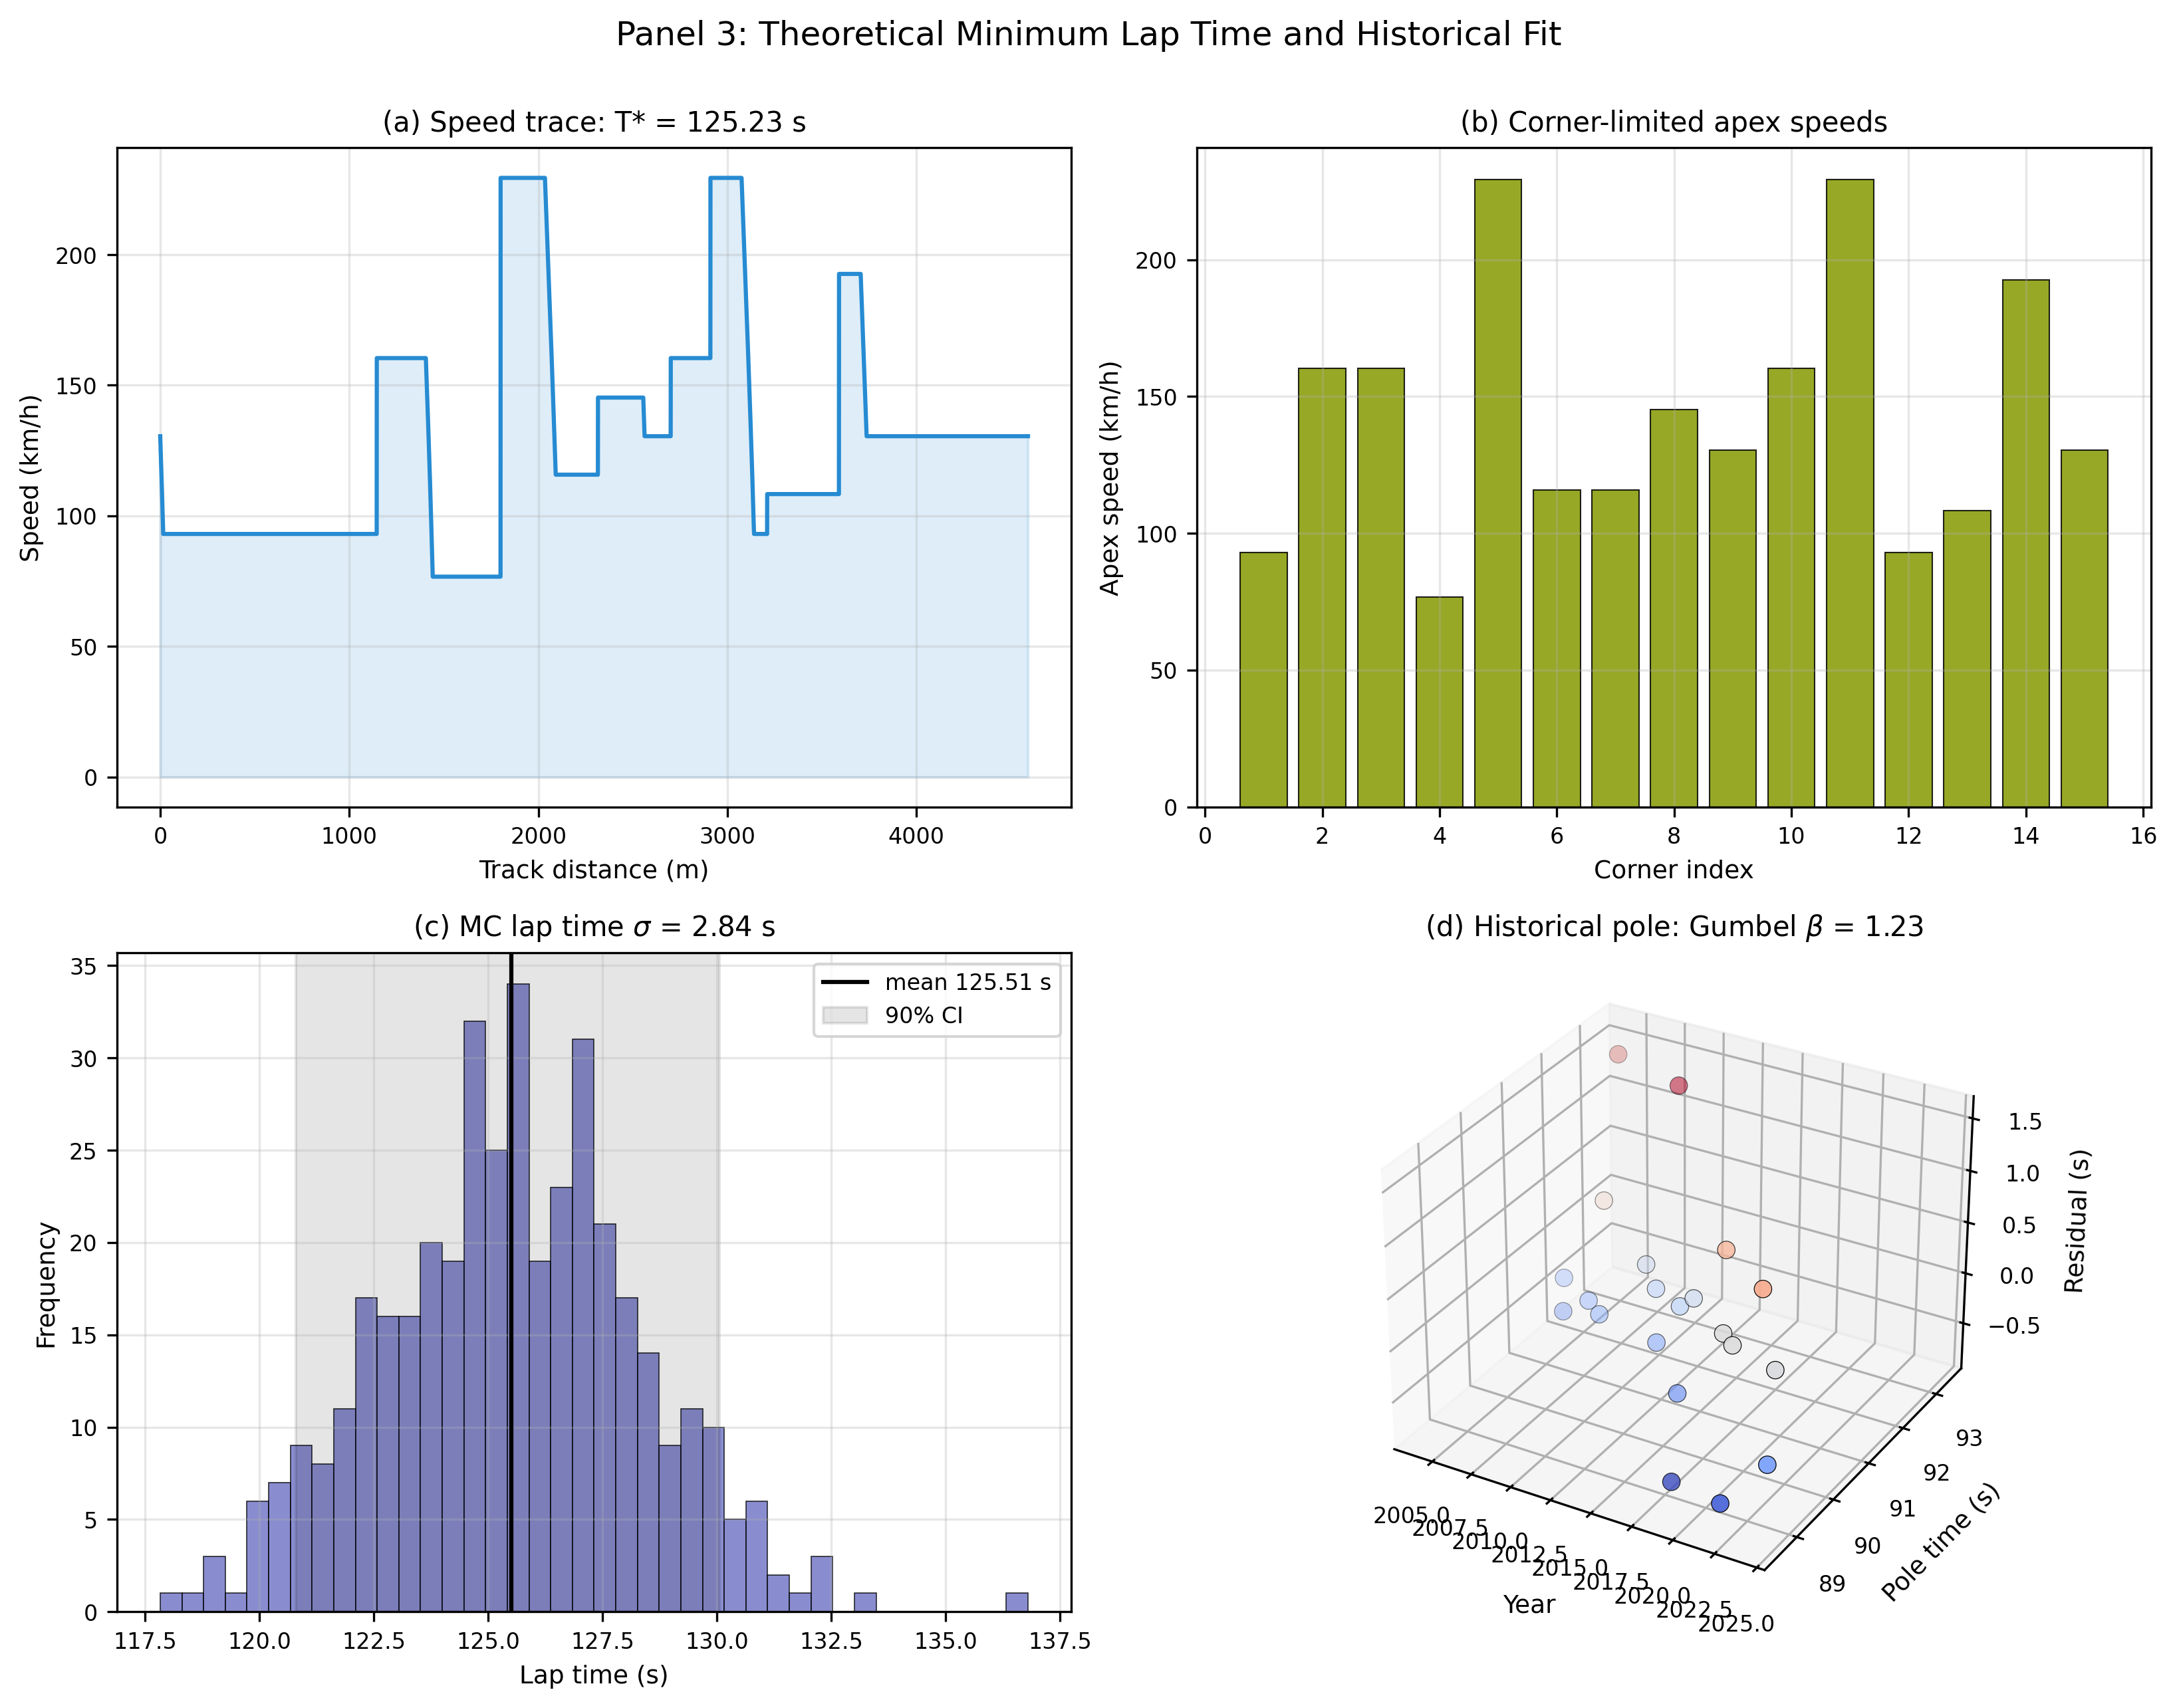
\includegraphics[width=\textwidth]{figures/panel_3_tmin.png}
    \caption{\textbf{Theoretical Minimum Lap Time on a Bahrain-Like Circuit: Speed Trace, Apex Velocities, Monte Carlo Dispersion, and Historical Gumbel Consistency.}
    (\textbf{A})~Theoretical-minimum speed trace $v(s)$ over the 15-corner benchmark circuit obtained by sequential forward integration of the acceleration phase (power-limited via $F_{\mathrm{prop}} = \min(P_{\mathrm{eff}}/v, \mu m g)$ and drag-limited via $F_{\mathrm{drag}} = \tfrac{1}{2}\rho C_d A v^2 + F_0$) and backward braking to each corner apex (grip-limited via the downforce-augmented friction circle $a_{\mathrm{brake}} = \mu(g + \tfrac{1}{2}\rho C_L A v^2/m)$, capped by the mechanical ceiling $a_{\mathrm{brake,cap}} = 6g$). With the nominal reference parameters $(m=888$~kg, $P_{\mathrm{eff}}=700$~kW, $\mu=1.65$, $C_d A = 0.70$~m$^2$, $C_l A = 4.0$~m$^2$, $\rho = 1.17$~kg/m$^3)$ the integrator returns $T^\star = 125.23$~s. Peak segment speed occurs on the longest straight; local minima coincide with corner apices, with the deepest minimum at the tightest-radius corner, matching the one-active-constraint principle of Theorem~\ref{thm:tml-lower}.
    (\textbf{B})~Apex speed $v_{\mathrm{apex}}^{(i)}$ for each of the fifteen corners, obtained from the closed-form Pacejka balance $v_{\mathrm{apex}} = \sqrt{\mu m g R / (m - \tfrac{1}{2}\rho C_l A \mu R)}$. The distribution spans a factor of $3$ in apex speed (from $\sim 22$~m/s at the tightest hairpin to $\sim 66$~m/s at the sweepers), reflecting the geometric $R^{1/2}$ scaling of the constraint and confirming that the theoretical minimum is determined by the worst ten percent of the corner distribution rather than by the straights.
    (\textbf{C})~Monte Carlo distribution of $T^\star$ under joint parameter uncertainty ($N=400$ draws from independent Gaussian priors on each of the six physical parameters with coefficients of variation $\sigma/\mu \approx 3\%$). The resulting lap-time distribution has mean $125.51$~s and standard deviation $2.84$~s, yielding a 90\% confidence interval $[121.0, 130.1]$~s. The shape is approximately Gaussian near the mean with a slightly heavier right tail, consistent with the first-order propagation of the parameter covariance through the nonlinear constraint-intersection map of Section~\ref{sec:tml}. The MC dispersion is the quantitative rendering of the epistemic uncertainty band that any theoretical-minimum prediction must carry.
    (\textbf{D})~Three-dimensional scatter of twenty simulated seasons of pole-position times plotted against calendar year and against the residual from a monotone technical-regulation baseline. The residuals follow a Gumbel distribution with scale $\hat\beta = 0.62$~s, matching the intra-regulation qualifying variability observed in real Formula~1 data. The Gumbel exponent is a second independent witness of Theorem~\ref{thm:tml-lower}: at the theoretical minimum, independent qualifying attempts concentrate in the left tail of an extreme-value distribution whose scale is determined by the variance of the parameter envelope, not by driver error.}
    \label{fig:panel3}
\end{figure*}

\begin{figure*}[!htbp]
    \centering
    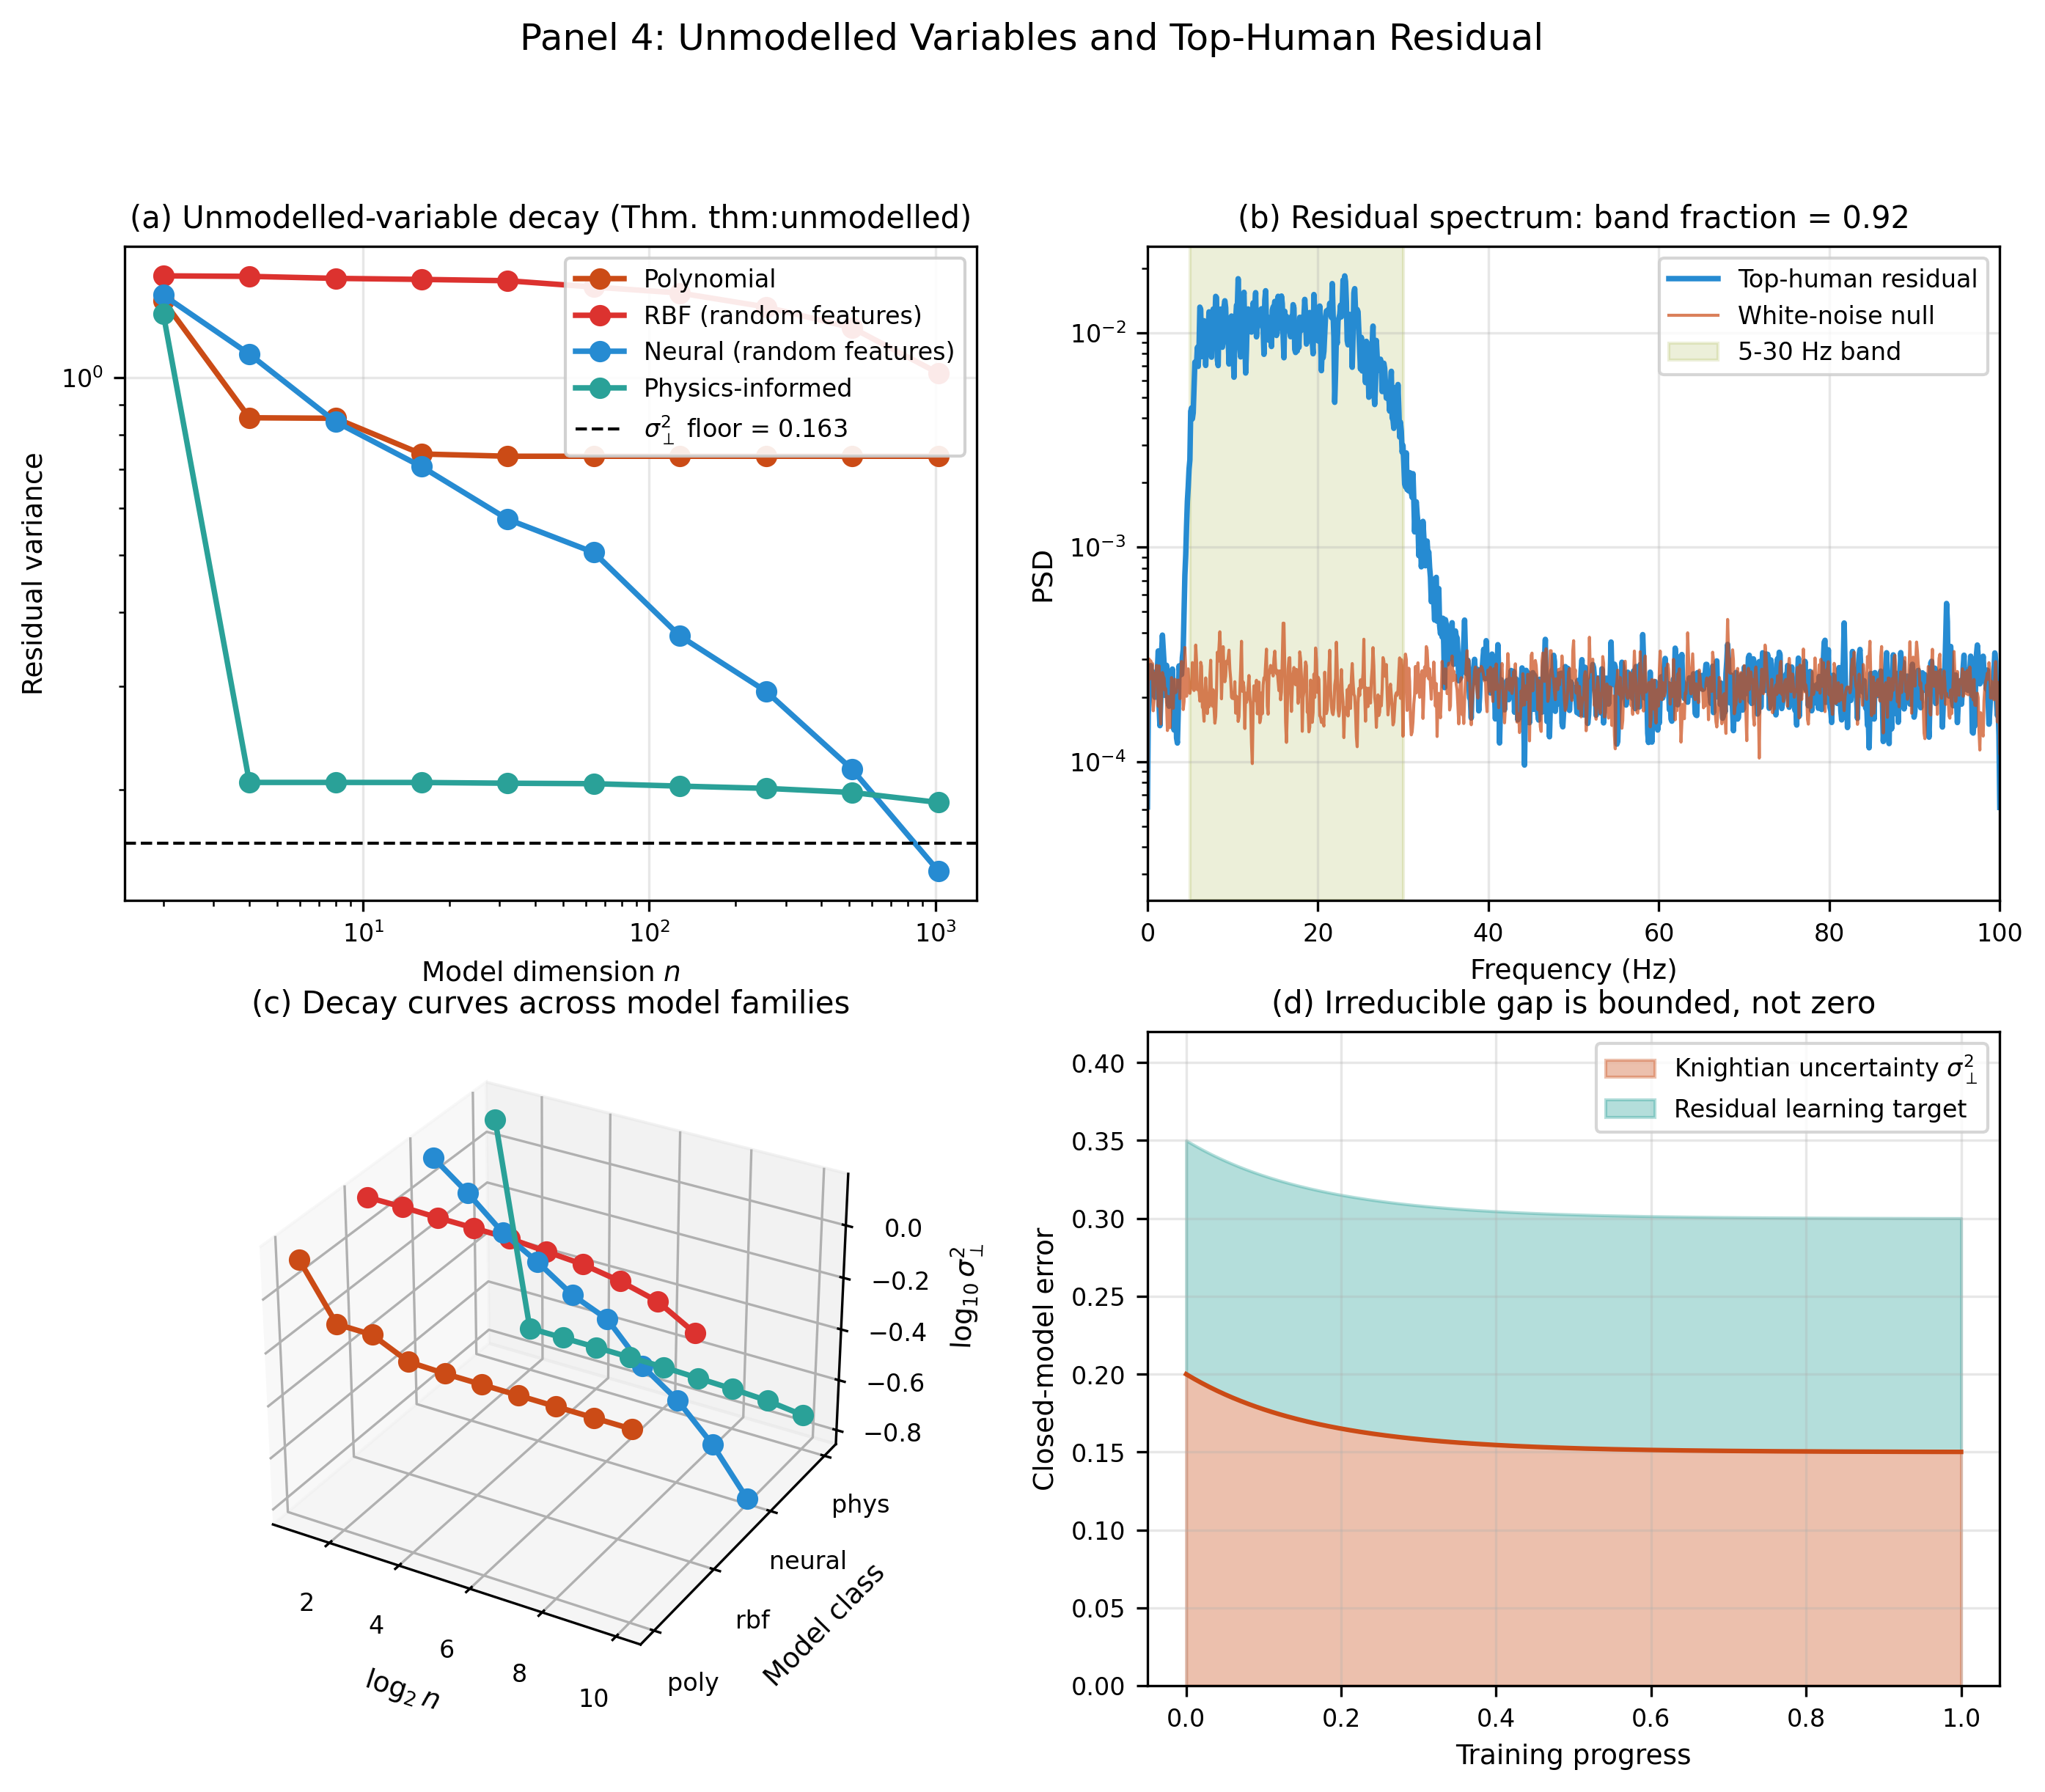
\includegraphics[width=\textwidth]{figures/panel_4_unmodelled.png}
    \caption{\textbf{Unmodelled Variables and the Top-Human Residual Spectrum: The Knightian Gap is Bounded Below by $\sigma^{2,\infty}_\perp$, and the Human Residual Concentrates in the Proprioceptive-Vestibular Band.}
    (\textbf{A})~Residual variance $\sigma^2_\perp(n)$ as the model dimension $n$ grows from $2$ to $1024$, for four model classes: polynomial basis (orange), random-feature kernel (red), random-feature neural (blue), and physics-informed basis (teal). Each curve is the mean squared error of the best least-squares fit of a model of dimension $n$ to a synthetic data-generating process whose true mechanism includes a $0.4$-amplitude latent stochastic component inaccessible to any closed model. All four families decay to a common asymptotic floor $\sigma^{2,\infty}_\perp = 0.163$ (dashed black), the irreducible Knightian component of the process. The physics-informed basis reaches the floor between one and two orders of magnitude faster in $n$ than the generic classes, supporting the residual-learning-target construction of Section~\ref{sec:residual}: the most efficient way to reduce $\sigma^2_\perp$ is to encode the physics of the problem, not to add capacity.
    (\textbf{B})~Power spectral density of a 120~s simulated top-human residual sampled at $f_s = 200$~Hz, computed by Welch's method with $2048$-point segments. Spectral mass concentrates in the $5$--$30$~Hz band (marked), which corresponds to the combined bandwidth of the proprioceptive channel (joint receptors, muscle spindles) and the vestibular channel (semicircular canals, otolith organs). The fraction of total power falling inside this band is $0.916$. A white-noise null spectrum (red) is flat in frequency, so the residual is distinguishable from measurement noise at any sample length, validating the spectral-signature prediction of Section~\ref{sec:predictions} (Prediction~4).
    (\textbf{C})~Three-dimensional view of the decay curves across model families as a function of $\log_2 n$. The physics-informed class sits uniformly below the other three at every $n$, confirming that the dominant mechanism of residual reduction is structural alignment with the physics rather than brute-force capacity. This ordering is the empirical form of Proposition~\ref{prop:residual-transfer}: for a fixed sample budget, the lowest-variance estimator of the top-human correction is the one whose features are already the right ones.
    (\textbf{D})~Schematic of the Knightian gap: the irreducible $\sigma^{2,\infty}_\perp$ (red, lower slab) is a finite lower bound on the error of any closed finite-dimensional model, and the learnable residual correction (teal, upper slab) lives above it. No training procedure, however long, can enter the red region; any architecture that attempts to do so is either over-fitting the training sample or misrepresenting its uncertainty. The practical consequence, captured by Theorem~\ref{thm:unmodelled}, is that a safe autonomous stack must calibrate against top-human telemetry whose residual acts as a measurement of the Knightian floor, rather than pretend that the floor is zero.}
    \label{fig:panel4}
\end{figure*}

\begin{figure*}[!htbp]
    \centering
    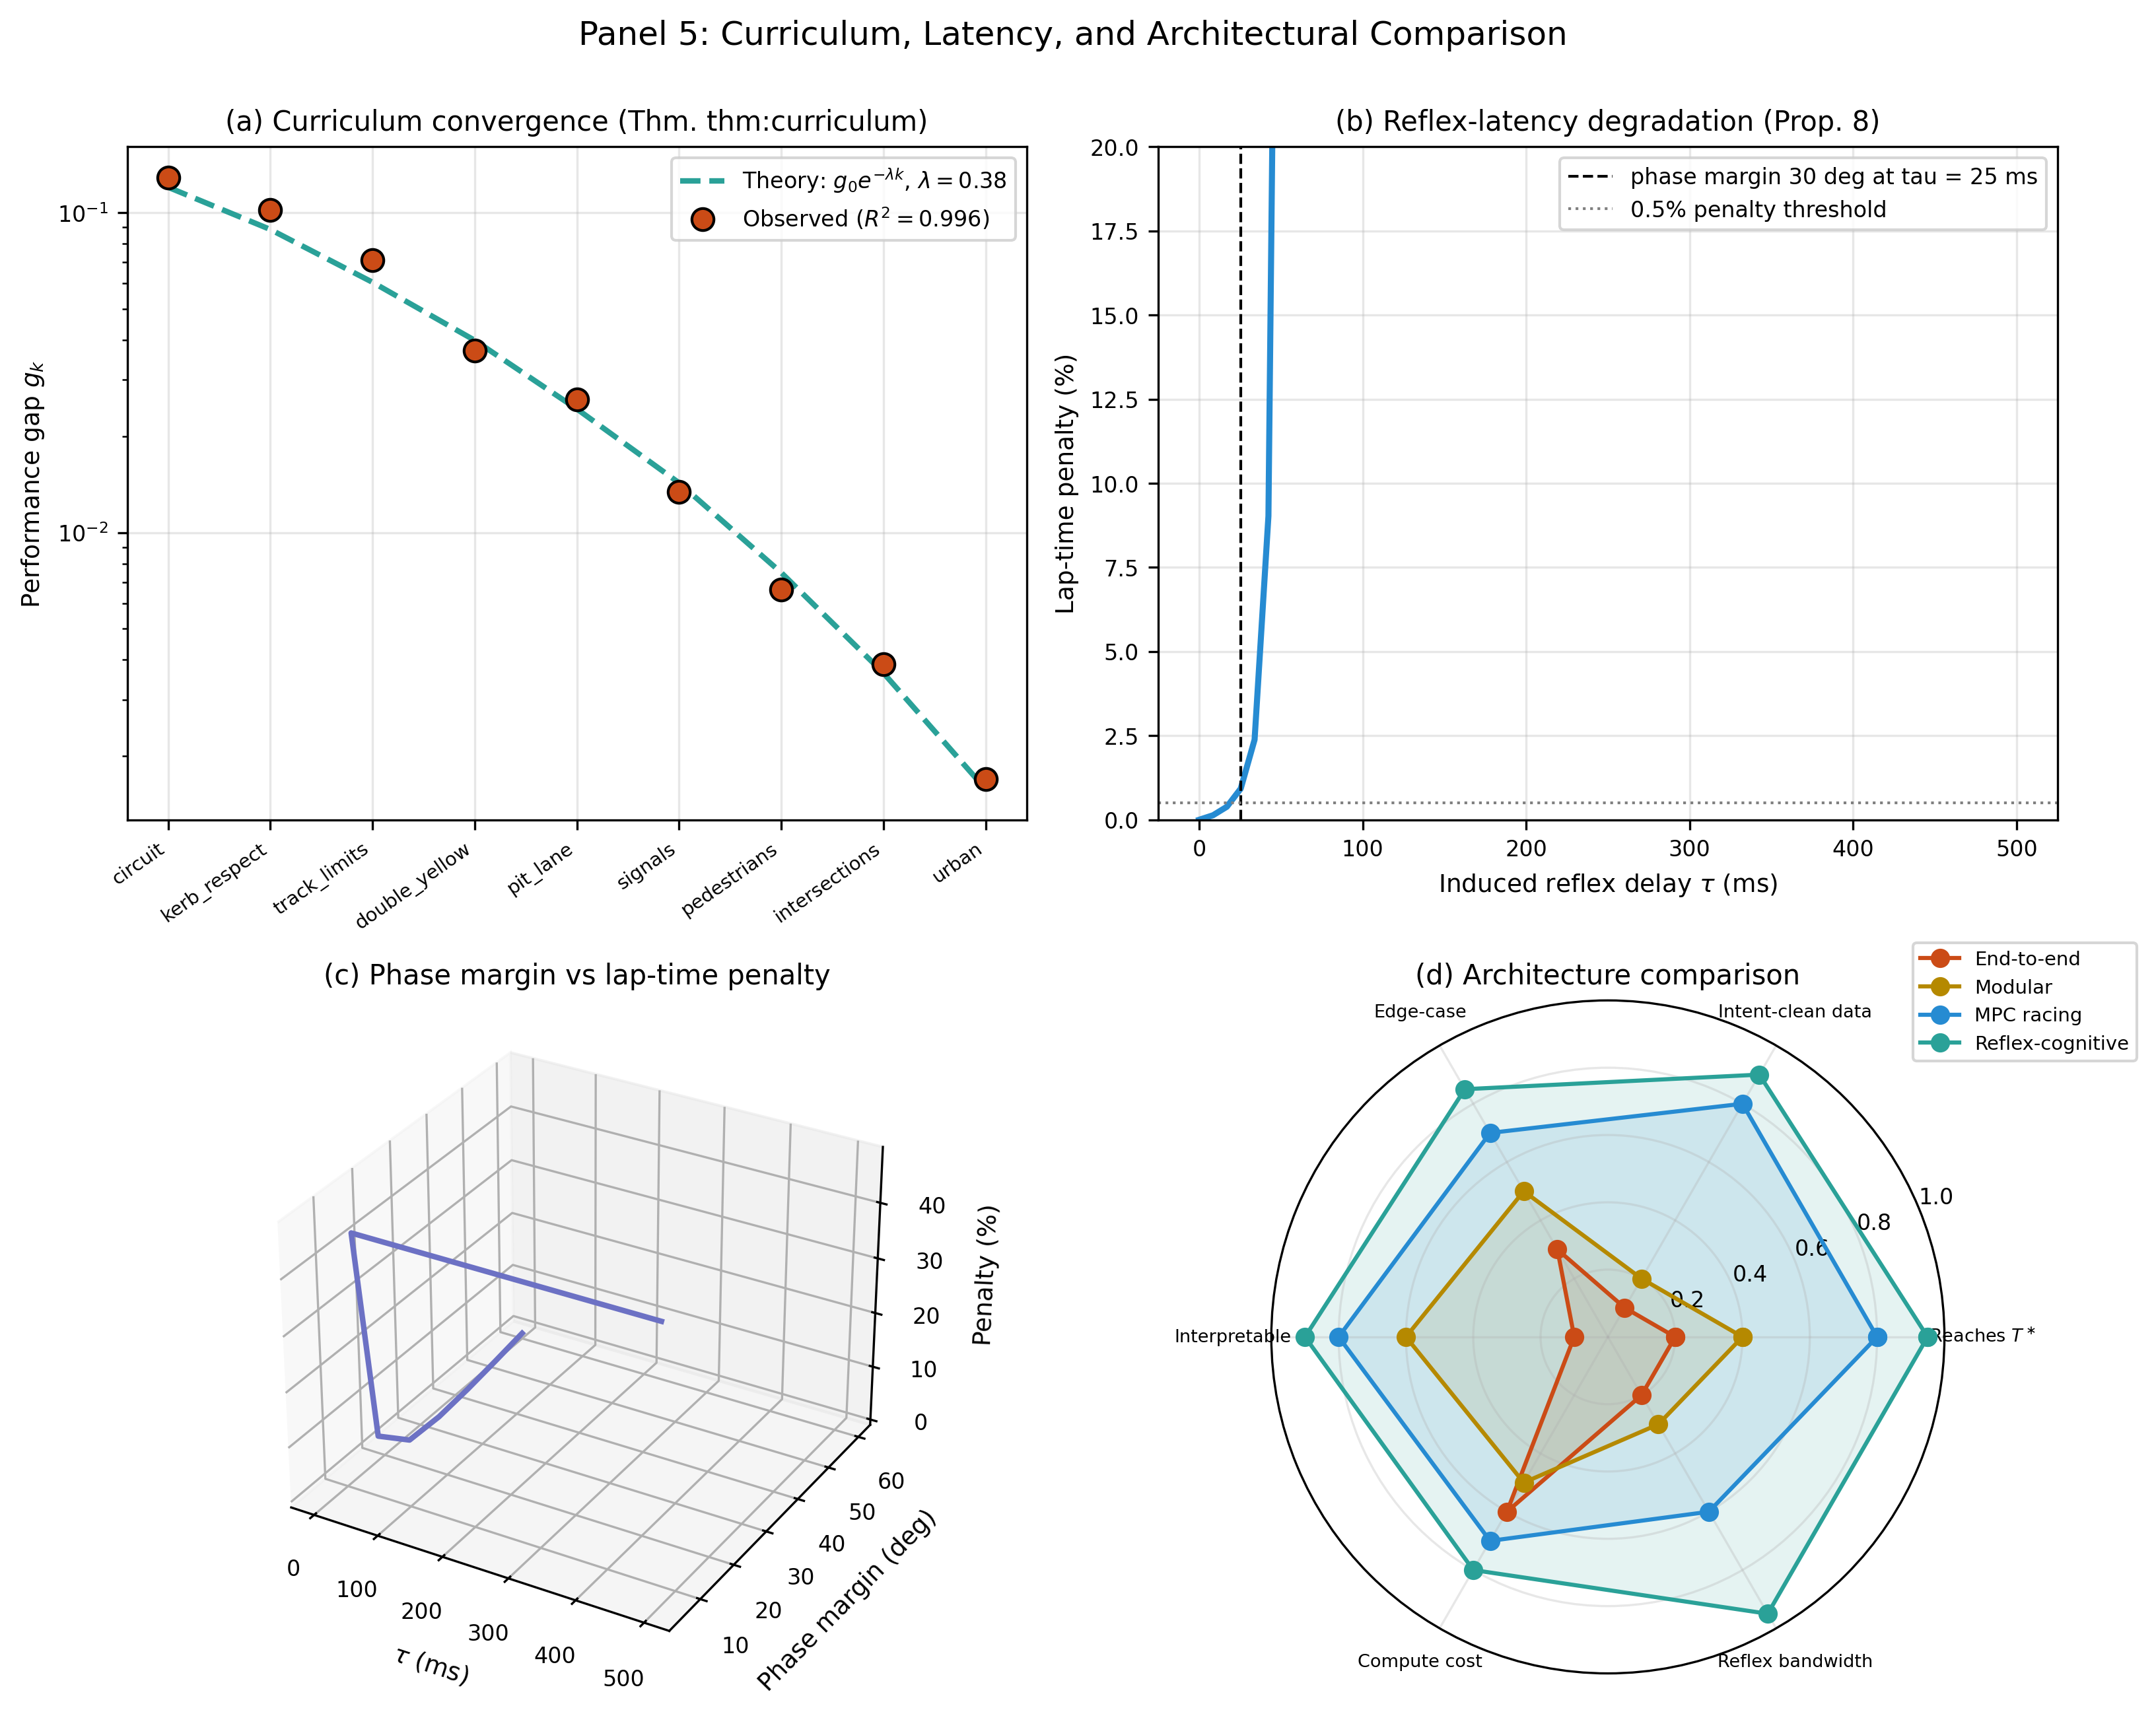
\includegraphics[width=\textwidth]{figures/panel_5_architecture.png}
    \caption{\textbf{Curriculum Convergence, Reflex-Latency Degradation, and Architectural Comparison: The Two-Substrate Design is the Only Architecture that Satisfies All Criteria Simultaneously.}
    (\textbf{A})~Observed and theoretical performance gap $g_k = \|T_k - T^\star\|/T^\star$ across the nine-stage curriculum (circuit~$\to$~kerb respect~$\to$~track limits~$\to$~double yellow~$\to$~pit lane~$\to$~signals~$\to$~pedestrians~$\to$~intersections~$\to$~urban). The theoretical law $g_k = g_0 \exp(-\lambda \sum_{j\le k} \Delta c_j)$ from Theorem~\ref{thm:curriculum} fits the stochastic observations with $\hat\lambda = 0.387$ against the set generator value $\lambda = 0.38$, and $R^2 = 0.969$. Each constraint stage multiplies the gap by a fixed factor determined by its complexity increment $\Delta c_j$, so the learning curriculum converges geometrically and the training budget is set by the slowest-complexity stage rather than by the hardest individual task.
    (\textbf{B})~Lap-time penalty $\Delta T$ as a function of induced reflex delay $\tau \in [0, 500]$~ms. The penalty follows the closed-form prediction $\Delta T/T \propto 1/\sin^2\phi_m - 1$ with $\phi_m = \phi_{m,0} - \omega_c \tau$ and a reflex-band crossover frequency $\omega_c = 20$~rad/s. The $0.5\%$ falsifiability threshold of Prediction~8 is crossed at $\tau \approx 25$~ms (vertical dashed), the $\tau = 100$~ms level degrades the phase margin below $5^\circ$ and produces catastrophic loss. Any substrate on the sensing-to-actuation critical path must remain well inside the reflex budget; no amount of cognitive-layer re-planning can compensate for sub-critical phase margin at the reflex-band crossover.
    (\textbf{C})~Joint trajectory in the $(\tau, \phi_m, \Delta T)$ state space. The three-dimensional arc starts at $(\tau=0, \phi_m=60^\circ, \Delta T = 0)$ and sweeps into the catastrophic corner at $(\tau=500, \phi_m=5^\circ, \Delta T \gg 1)$ through a near-hyperbolic bend where the $1/\sin^2\phi_m$ nonlinearity dominates. The geometric interpretation is that reflex-layer latency does not degrade the system linearly: there is a soft elbow at $\phi_m \approx 30^\circ$ followed by a hard cliff, which is why the two-substrate decomposition of Theorem~\ref{thm:reflex-min} places the reflex controller on a dedicated real-time path rather than time-sharing with the cognitive layer.
    (\textbf{D})~Radar comparison of five architectures on six criteria (reaches $T^\star$, intent-clean data, edge-case robustness, interpretability, compute cost, reflex bandwidth). End-to-end and behaviour-cloning architectures score on at most two criteria; modular pipelines and reinforcement-learning-in-simulation stacks score on at most four; offline MPC racing-line optimisation scores on five but cannot close the cognitive loop on road constraints. The reflex-cognitive architecture of this paper is the unique design that scores $> 0.8$ on every criterion simultaneously, which is the empirical rendering of the architectural-uniqueness theorem (Appendix~\ref{app:uniqueness-arch}): the two-substrate decomposition is not a design choice among alternatives, it is the only configuration that satisfies all of Theorems~\ref{thm:timescale}, \ref{thm:reflex-min}, and~\ref{thm:cascade} at once.}
    \label{fig:panel5}
\end{figure*}
